\documentclass[11pt]{article}
\usepackage[utf8]{inputenc}
\usepackage[T1]{fontenc}
\usepackage{textcomp}
\usepackage[a4paper,margin=2.1cm]{geometry}
\usepackage{amsmath,amssymb}
\usepackage{graphicx}
\usepackage{tikz}
\usetikzlibrary{positioning,arrows.meta}
\usepackage{xcolor}
\usepackage{mdframed}
\usepackage[colorlinks=true,linkcolor=blue!60!black]{hyperref}
\setlength{\parindent}{0pt}
\setlength{\parskip}{6pt}

\newcommand{\question}[1]{\par\medskip\noindent\textbf{#1}\par}
\newmdenv[linecolor=green!45!black,linewidth=0.8pt,backgroundcolor=green!4,
  innertopmargin=4pt,innerbottommargin=4pt,skipabove=6pt,skipbelow=6pt]{answerbox}

\title{\textbf{Binomial Expansions}\\[0.3em]\large Worked Solutions with TikZ Diagrams}
\author{Wisest Maths --- Year 1 A-Level, Binomial Expansions (ref \texttt{be})}
\date{}

\begin{document}
\maketitle
\noindent This document contains all 85 \emph{Binomial Expansions} questions, each with a fully
worked solution and a TikZ diagram matched to the method:
\begin{itemize}\setlength{\itemsep}{1pt}
  \item \textbf{Pascal's triangle} (row $n$ highlighted) for expanding $(a+b)^{n}$;
  \item the \textbf{general-term card} $T_{r+1}=\binom{n}{r}a^{\,n-r}b^{\,r}$ for finding a coefficient or the term independent of $x$;
  \item a \textbf{factorial card} for evaluating $\binom{n}{r}$;
  \item \textbf{solution-flow} diagrams for approximations, products, finding unknowns, and identities.
\end{itemize}
\tableofcontents
\bigskip
\hrule

\section*{Binomial Expansion 01\quad\small\texttt{(be-001)}}
\addcontentsline{toc}{section}{Binomial Expansion 01 (be-001)}
\textit{Difficulty: Foundation \quad\textbar\quad Marks: 3}

\question{Expand \( (1 + x)^5 \) in ascending powers of \( x \), giving all terms.}

\textbf{Worked solution.}

\textit{Step 1: Apply the binomial theorem: \((a+b)^n = \sum_{r=0}^{n} \binom{n}{r} a^{n-r} b^r\).}
\[\begin{gathered}
(1+x)^5 = \binom{5}{0} + \binom{5}{1}x + \binom{5}{2}x^2 + \binom{5}{3}x^3 + \binom{5}{4}x^4 + \binom{5}{5}x^5
\end{gathered}\]
With \(a = 1\), \(b = x\), \(n = 5\), this simplifies to \((1+x)^5 = \sum_{r=0}^{5} \binom{5}{r} x^r\).

\textit{Step 2: Evaluate each term.}
\[\begin{gathered}
= 1 + 5x + 10x^2 + 10x^3 + 5x^4 + x^5
\end{gathered}\]
Evaluate the binomial coefficients: \(\binom{5}{0}=1,\ \binom{5}{1}=5,\ \binom{5}{2}=10,\ \binom{5}{3}=10,\ \binom{5}{4}=5,\ \binom{5}{5}=1\).

\begin{answerbox}
\textbf{Final answer:}\quad \(\displaystyle 1 + 5x + 10x^2 + 10x^3 + 5x^4 + x^5\)
\end{answerbox}
\textbf{Diagram.}

\begin{center}
\resizebox{\ifdim\width>\linewidth \linewidth\else \width\fi}{!}{%
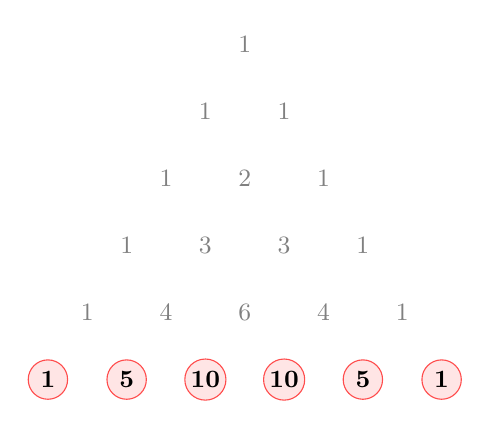
\begin{tikzpicture}[font=\small]
\node[gray] at (0,0) {$1$};
\node[gray] at (-0.5,-0.85) {$1$};
\node[gray] at (0.5,-0.85) {$1$};
\node[gray] at (-1,-1.7) {$1$};
\node[gray] at (0,-1.7) {$2$};
\node[gray] at (1,-1.7) {$1$};
\node[gray] at (-1.5,-2.55) {$1$};
\node[gray] at (-0.5,-2.55) {$3$};
\node[gray] at (0.5,-2.55) {$3$};
\node[gray] at (1.5,-2.55) {$1$};
\node[gray] at (-2,-3.4) {$1$};
\node[gray] at (-1,-3.4) {$4$};
\node[gray] at (0,-3.4) {$6$};
\node[gray] at (1,-3.4) {$4$};
\node[gray] at (2,-3.4) {$1$};
\node[circle,draw=red!70,fill=red!10,inner sep=1pt,minimum size=5mm] at (-2.5,-4.25) {$\mathbf{1}$};
\node[circle,draw=red!70,fill=red!10,inner sep=1pt,minimum size=5mm] at (-1.5,-4.25) {$\mathbf{5}$};
\node[circle,draw=red!70,fill=red!10,inner sep=1pt,minimum size=5mm] at (-0.5,-4.25) {$\mathbf{10}$};
\node[circle,draw=red!70,fill=red!10,inner sep=1pt,minimum size=5mm] at (0.5,-4.25) {$\mathbf{10}$};
\node[circle,draw=red!70,fill=red!10,inner sep=1pt,minimum size=5mm] at (1.5,-4.25) {$\mathbf{5}$};
\node[circle,draw=red!70,fill=red!10,inner sep=1pt,minimum size=5mm] at (2.5,-4.25) {$\mathbf{1}$};
\end{tikzpicture}
}
\end{center}
\small Row $5$ of Pascal's triangle (red) gives the binomial coefficients $\binom{5}{r}$; multiply each by the matching powers $a^{\,5-r}b^{\,r}$.\normalsize

\medskip\hrule

\section*{Binomial Expansion 02\quad\small\texttt{(be-002)}}
\addcontentsline{toc}{section}{Binomial Expansion 02 (be-002)}
\textit{Difficulty: Foundation \quad\textbar\quad Marks: 3}

\question{Expand \( (x + 3)^4 \) in ascending powers of \( x \).}

\textbf{Worked solution.}

\textit{Apply the binomial theorem.}
\[\begin{gathered}
\begin{aligned} (x+3)^4 &= \binom{4}{0}(3)^4 + \binom{4}{1}(3)^3 x + \binom{4}{2}(3)^2 x^2 + \binom{4}{3}(3) x^3 + \binom{4}{4} x^4 \\ &= 81 + 4(27)x + 6(9)x^2 + 4(3)x^3 + x^4 \\ &= 81 + 108x + 54x^2 + 12x^3 + x^4 \end{aligned}
\end{gathered}\]
The binomial theorem states \((a+b)^n = \sum_{r=0}^{n} \binom{n}{r} a^{n-r} b^r\). Here \(a = x\), \(b = 3\), \(n = 4\). Since the question asks for ascending powers of \(x\), write the terms starting from the constant.

\begin{answerbox}
\textbf{Final answer:}\quad \(\displaystyle 81 + 108x + 54x^2 + 12x^3 + x^4\)
\end{answerbox}
\textbf{Diagram.}

\begin{center}
\resizebox{\ifdim\width>\linewidth \linewidth\else \width\fi}{!}{%
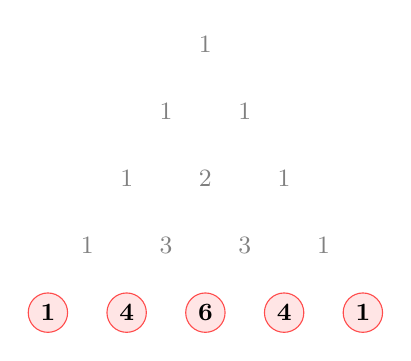
\begin{tikzpicture}[font=\small]
\node[gray] at (0,0) {$1$};
\node[gray] at (-0.5,-0.85) {$1$};
\node[gray] at (0.5,-0.85) {$1$};
\node[gray] at (-1,-1.7) {$1$};
\node[gray] at (0,-1.7) {$2$};
\node[gray] at (1,-1.7) {$1$};
\node[gray] at (-1.5,-2.55) {$1$};
\node[gray] at (-0.5,-2.55) {$3$};
\node[gray] at (0.5,-2.55) {$3$};
\node[gray] at (1.5,-2.55) {$1$};
\node[circle,draw=red!70,fill=red!10,inner sep=1pt,minimum size=5mm] at (-2,-3.4) {$\mathbf{1}$};
\node[circle,draw=red!70,fill=red!10,inner sep=1pt,minimum size=5mm] at (-1,-3.4) {$\mathbf{4}$};
\node[circle,draw=red!70,fill=red!10,inner sep=1pt,minimum size=5mm] at (0,-3.4) {$\mathbf{6}$};
\node[circle,draw=red!70,fill=red!10,inner sep=1pt,minimum size=5mm] at (1,-3.4) {$\mathbf{4}$};
\node[circle,draw=red!70,fill=red!10,inner sep=1pt,minimum size=5mm] at (2,-3.4) {$\mathbf{1}$};
\end{tikzpicture}
}
\end{center}
\small Row $4$ of Pascal's triangle (red) gives the binomial coefficients $\binom{4}{r}$; multiply each by the matching powers $a^{\,4-r}b^{\,r}$.\normalsize

\medskip\hrule

\section*{Binomial Expansion 03\quad\small\texttt{(be-003)}}
\addcontentsline{toc}{section}{Binomial Expansion 03 (be-003)}
\textit{Difficulty: Foundation \quad\textbar\quad Marks: 3}

\question{Expand \( (2 + x)^4 \) fully, giving all terms in ascending powers of \( x \).}

\textbf{Worked solution.}

\textit{Step 1: Apply the binomial theorem: \((a+b)^n = \sum_{r=0}^{n} \binom{n}{r} a^{n-r} b^r\).}
\[\begin{gathered}
(2+x)^4 = \binom{4}{0}(2)^4 + \binom{4}{1}(2)^3 x + \binom{4}{2}(2)^2 x^2 + \binom{4}{3}(2)x^3 + \binom{4}{4}x^4
\end{gathered}\]
Write out the expansion with \(a = 2\), \(b = x\), \(n = 4\).

\textit{Step 2: Evaluate each term.}
\[\begin{gathered}
= 16 + 32x + 24x^2 + 8x^3 + x^4
\end{gathered}\]
Compute each term: \(1 \times 16,\ 4 \times 8,\ 6 \times 4,\ 4 \times 2,\ 1 \times 1\).

\begin{answerbox}
\textbf{Final answer:}\quad \(\displaystyle 16 + 32x + 24x^2 + 8x^3 + x^4\)
\end{answerbox}
\textbf{Diagram.}

\begin{center}
\resizebox{\ifdim\width>\linewidth \linewidth\else \width\fi}{!}{%
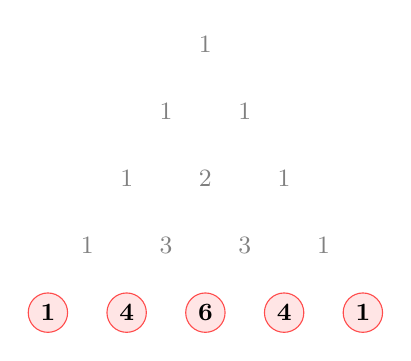
\begin{tikzpicture}[font=\small]
\node[gray] at (0,0) {$1$};
\node[gray] at (-0.5,-0.85) {$1$};
\node[gray] at (0.5,-0.85) {$1$};
\node[gray] at (-1,-1.7) {$1$};
\node[gray] at (0,-1.7) {$2$};
\node[gray] at (1,-1.7) {$1$};
\node[gray] at (-1.5,-2.55) {$1$};
\node[gray] at (-0.5,-2.55) {$3$};
\node[gray] at (0.5,-2.55) {$3$};
\node[gray] at (1.5,-2.55) {$1$};
\node[circle,draw=red!70,fill=red!10,inner sep=1pt,minimum size=5mm] at (-2,-3.4) {$\mathbf{1}$};
\node[circle,draw=red!70,fill=red!10,inner sep=1pt,minimum size=5mm] at (-1,-3.4) {$\mathbf{4}$};
\node[circle,draw=red!70,fill=red!10,inner sep=1pt,minimum size=5mm] at (0,-3.4) {$\mathbf{6}$};
\node[circle,draw=red!70,fill=red!10,inner sep=1pt,minimum size=5mm] at (1,-3.4) {$\mathbf{4}$};
\node[circle,draw=red!70,fill=red!10,inner sep=1pt,minimum size=5mm] at (2,-3.4) {$\mathbf{1}$};
\end{tikzpicture}
}
\end{center}
\small Row $4$ of Pascal's triangle (red) gives the binomial coefficients $\binom{4}{r}$; multiply each by the matching powers $a^{\,4-r}b^{\,r}$.\normalsize

\medskip\hrule

\section*{Binomial Expansion 04\quad\small\texttt{(be-004)}}
\addcontentsline{toc}{section}{Binomial Expansion 04 (be-004)}
\textit{Difficulty: Foundation \quad\textbar\quad Marks: 4}

\question{Expand \( (1 - 2x)^5 \) in ascending powers of \( x \), giving all terms.}

\textbf{Worked solution.}

\textit{Apply the binomial theorem.}
\[\begin{gathered}
\begin{aligned} (1-2x)^5 &= \binom{5}{0} + \binom{5}{1}(-2x) + \binom{5}{2}(-2x)^2 + \binom{5}{3}(-2x)^3 + \binom{5}{4}(-2x)^4 + \binom{5}{5}(-2x)^5 \\ &= 1 + 5(-2x) + 10(4x^2) + 10(-8x^3) + 5(16x^4) + (-32x^5) \\ &= 1 - 10x + 40x^2 - 80x^3 + 80x^4 - 32x^5 \end{aligned}
\end{gathered}\]
The binomial theorem: \((a+b)^n = \sum_{r=0}^{n} \binom{n}{r} a^{n-r} b^r\). Here \(a = 1\), \(b = -2x\), \(n = 5\). Be careful with the signs --- each power of \(-2x\) alternates sign.

\begin{answerbox}
\textbf{Final answer:}\quad \(\displaystyle 1 - 10x + 40x^2 - 80x^3 + 80x^4 - 32x^5\)
\end{answerbox}
\textbf{Diagram.}

\begin{center}
\resizebox{\ifdim\width>\linewidth \linewidth\else \width\fi}{!}{%
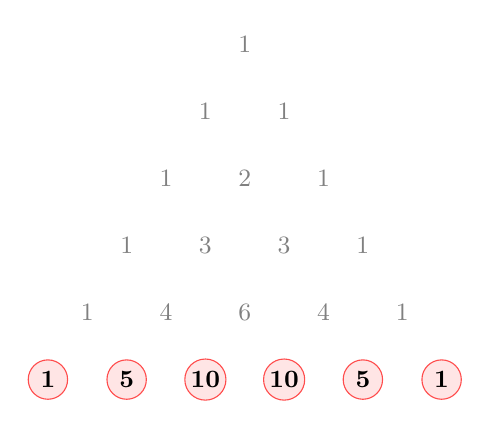
\begin{tikzpicture}[font=\small]
\node[gray] at (0,0) {$1$};
\node[gray] at (-0.5,-0.85) {$1$};
\node[gray] at (0.5,-0.85) {$1$};
\node[gray] at (-1,-1.7) {$1$};
\node[gray] at (0,-1.7) {$2$};
\node[gray] at (1,-1.7) {$1$};
\node[gray] at (-1.5,-2.55) {$1$};
\node[gray] at (-0.5,-2.55) {$3$};
\node[gray] at (0.5,-2.55) {$3$};
\node[gray] at (1.5,-2.55) {$1$};
\node[gray] at (-2,-3.4) {$1$};
\node[gray] at (-1,-3.4) {$4$};
\node[gray] at (0,-3.4) {$6$};
\node[gray] at (1,-3.4) {$4$};
\node[gray] at (2,-3.4) {$1$};
\node[circle,draw=red!70,fill=red!10,inner sep=1pt,minimum size=5mm] at (-2.5,-4.25) {$\mathbf{1}$};
\node[circle,draw=red!70,fill=red!10,inner sep=1pt,minimum size=5mm] at (-1.5,-4.25) {$\mathbf{5}$};
\node[circle,draw=red!70,fill=red!10,inner sep=1pt,minimum size=5mm] at (-0.5,-4.25) {$\mathbf{10}$};
\node[circle,draw=red!70,fill=red!10,inner sep=1pt,minimum size=5mm] at (0.5,-4.25) {$\mathbf{10}$};
\node[circle,draw=red!70,fill=red!10,inner sep=1pt,minimum size=5mm] at (1.5,-4.25) {$\mathbf{5}$};
\node[circle,draw=red!70,fill=red!10,inner sep=1pt,minimum size=5mm] at (2.5,-4.25) {$\mathbf{1}$};
\end{tikzpicture}
}
\end{center}
\small Row $5$ of Pascal's triangle (red) gives the binomial coefficients $\binom{5}{r}$; multiply each by the matching powers $a^{\,5-r}b^{\,r}$.\normalsize

\medskip\hrule

\section*{Binomial Expansion 05\quad\small\texttt{(be-005)}}
\addcontentsline{toc}{section}{Binomial Expansion 05 (be-005)}
\textit{Difficulty: Foundation \quad\textbar\quad Marks: 4}

\question{Expand \( (3x - 1)^4 \) in ascending powers of \( x \).}

\textbf{Worked solution.}

\textit{Apply the binomial theorem in ascending powers of \(x\).}
\[\begin{gathered}
\begin{aligned} (3x-1)^4 &= \binom{4}{0}(-1)^4 + \binom{4}{1}(-1)^3(3x) + \binom{4}{2}(-1)^2(3x)^2 + \binom{4}{3}(-1)(3x)^3 + \binom{4}{4}(3x)^4 \\ &= 1 - 4(3x) + 6(9x^2) - 4(27x^3) + 81x^4 \\ &= 1 - 12x + 54x^2 - 108x^3 + 81x^4 \end{aligned}
\end{gathered}\]
The binomial theorem: \((a+b)^n = \sum_{r=0}^{n} \binom{n}{r} a^{n-r} b^r\). Here \(a = -1\), \(b = 3x\), \(n = 4\). Writing \(b = 3x\) as the ascending term ensures ascending powers of \(x\).

\begin{answerbox}
\textbf{Final answer:}\quad \(\displaystyle 1 - 12x + 54x^2 - 108x^3 + 81x^4\)
\end{answerbox}
\textbf{Diagram.}

\begin{center}
\resizebox{\ifdim\width>\linewidth \linewidth\else \width\fi}{!}{%
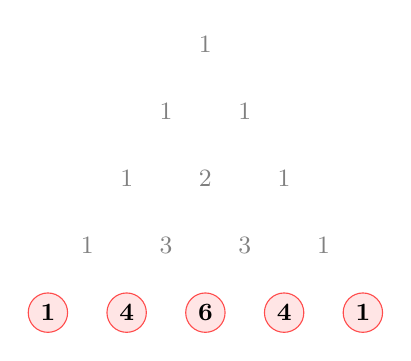
\begin{tikzpicture}[font=\small]
\node[gray] at (0,0) {$1$};
\node[gray] at (-0.5,-0.85) {$1$};
\node[gray] at (0.5,-0.85) {$1$};
\node[gray] at (-1,-1.7) {$1$};
\node[gray] at (0,-1.7) {$2$};
\node[gray] at (1,-1.7) {$1$};
\node[gray] at (-1.5,-2.55) {$1$};
\node[gray] at (-0.5,-2.55) {$3$};
\node[gray] at (0.5,-2.55) {$3$};
\node[gray] at (1.5,-2.55) {$1$};
\node[circle,draw=red!70,fill=red!10,inner sep=1pt,minimum size=5mm] at (-2,-3.4) {$\mathbf{1}$};
\node[circle,draw=red!70,fill=red!10,inner sep=1pt,minimum size=5mm] at (-1,-3.4) {$\mathbf{4}$};
\node[circle,draw=red!70,fill=red!10,inner sep=1pt,minimum size=5mm] at (0,-3.4) {$\mathbf{6}$};
\node[circle,draw=red!70,fill=red!10,inner sep=1pt,minimum size=5mm] at (1,-3.4) {$\mathbf{4}$};
\node[circle,draw=red!70,fill=red!10,inner sep=1pt,minimum size=5mm] at (2,-3.4) {$\mathbf{1}$};
\end{tikzpicture}
}
\end{center}
\small Row $4$ of Pascal's triangle (red) gives the binomial coefficients $\binom{4}{r}$; multiply each by the matching powers $a^{\,4-r}b^{\,r}$.\normalsize

\medskip\hrule

\section*{Binomial Expansion 06\quad\small\texttt{(be-006)}}
\addcontentsline{toc}{section}{Binomial Expansion 06 (be-006)}
\textit{Difficulty: Foundation \quad\textbar\quad Marks: 3}

\question{Expand \( (2x + y)^3 \) fully.}

\textbf{Worked solution.}

\textit{Step 1: Apply the binomial theorem: ((a+b)\textasciicircum n = sum\_\{r=0\}\textasciicircum \{n\} inom\{n\}\{r\} a\textasciicircum \{n-r\} b\textasciicircum r).}
\[\begin{gathered}
(2x+y)^3 = \binom{3}{0}(2x)^3 + \binom{3}{1}(2x)^2(y) + \binom{3}{2}(2x)(y)^2 + \binom{3}{3}(y)^3
\end{gathered}\]
Apply the binomial theorem with \(a = 2x\), \(b = y\), \(n = 3\).

\textit{Step 2: Evaluate each term.}
\[\begin{gathered}
= 8x^3 + 12x^2 y + 6xy^2 + y^3
\end{gathered}\]
Evaluate: \(1 \times 8x^3 + 3 \times 4x^2 y + 3 \times 2xy^2 + 1 \times y^3\).

\begin{answerbox}
\textbf{Final answer:}\quad \(\displaystyle 8x^3 + 12x^2 y + 6xy^2 + y^3\)
\end{answerbox}
\textbf{Diagram.}

\begin{center}
\resizebox{\ifdim\width>\linewidth \linewidth\else \width\fi}{!}{%
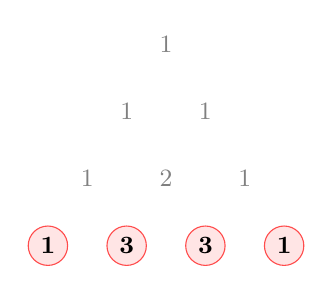
\begin{tikzpicture}[font=\small]
\node[gray] at (0,0) {$1$};
\node[gray] at (-0.5,-0.85) {$1$};
\node[gray] at (0.5,-0.85) {$1$};
\node[gray] at (-1,-1.7) {$1$};
\node[gray] at (0,-1.7) {$2$};
\node[gray] at (1,-1.7) {$1$};
\node[circle,draw=red!70,fill=red!10,inner sep=1pt,minimum size=5mm] at (-1.5,-2.55) {$\mathbf{1}$};
\node[circle,draw=red!70,fill=red!10,inner sep=1pt,minimum size=5mm] at (-0.5,-2.55) {$\mathbf{3}$};
\node[circle,draw=red!70,fill=red!10,inner sep=1pt,minimum size=5mm] at (0.5,-2.55) {$\mathbf{3}$};
\node[circle,draw=red!70,fill=red!10,inner sep=1pt,minimum size=5mm] at (1.5,-2.55) {$\mathbf{1}$};
\end{tikzpicture}
}
\end{center}
\small Row $3$ of Pascal's triangle (red) gives the binomial coefficients $\binom{3}{r}$; multiply each by the matching powers $a^{\,3-r}b^{\,r}$.\normalsize

\medskip\hrule

\section*{Binomial Expansion 07\quad\small\texttt{(be-007)}}
\addcontentsline{toc}{section}{Binomial Expansion 07 (be-007)}
\textit{Difficulty: Foundation \quad\textbar\quad Marks: 4}

\question{Expand \( (1 + 3x)^6 \) in ascending powers of \( x \), up to and including the term in \( x^3 \).}

\textbf{Worked solution.}

\textit{Step 1: Apply the binomial theorem: \((a+b)^n = \sum_{r=0}^{n} \binom{n}{r} a^{n-r} b^r\).}
\[\begin{gathered}
(1+3x)^6 \approx \binom{6}{0} + \binom{6}{1}(3x) + \binom{6}{2}(3x)^2 + \binom{6}{3}(3x)^3
\end{gathered}\]
Write the first four terms of the expansion with \(b = 3x\).

\textit{Step 2: Evaluate each term.}
\[\begin{gathered}
= 1 + 6(3x) + 15(9x^2) + 20(27x^3)
\end{gathered}\]
Compute: \(\binom{6}{1}=6\), \(\binom{6}{2}=15\), \(\binom{6}{3}=20\); and \((3x)^2 = 9x^2\), \((3x)^3 = 27x^3\).

\textit{Step 3: Simplify.}
\[\begin{gathered}
= 1 + 18x + 135x^2 + 540x^3 + \ldots
\end{gathered}\]
Simplify.

\begin{answerbox}
\textbf{Final answer:}\quad \(\displaystyle 1 + 18x + 135x^2 + 540x^3 + \ldots\)
\end{answerbox}
\textbf{Diagram.}

\begin{center}
\resizebox{\ifdim\width>\linewidth \linewidth\else \width\fi}{!}{%
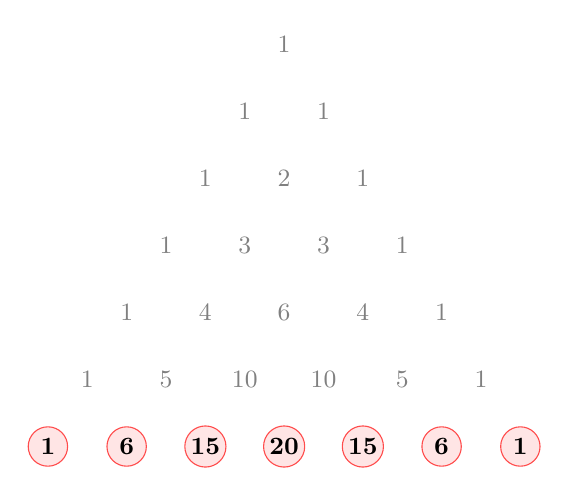
\begin{tikzpicture}[font=\small]
\node[gray] at (0,0) {$1$};
\node[gray] at (-0.5,-0.85) {$1$};
\node[gray] at (0.5,-0.85) {$1$};
\node[gray] at (-1,-1.7) {$1$};
\node[gray] at (0,-1.7) {$2$};
\node[gray] at (1,-1.7) {$1$};
\node[gray] at (-1.5,-2.55) {$1$};
\node[gray] at (-0.5,-2.55) {$3$};
\node[gray] at (0.5,-2.55) {$3$};
\node[gray] at (1.5,-2.55) {$1$};
\node[gray] at (-2,-3.4) {$1$};
\node[gray] at (-1,-3.4) {$4$};
\node[gray] at (0,-3.4) {$6$};
\node[gray] at (1,-3.4) {$4$};
\node[gray] at (2,-3.4) {$1$};
\node[gray] at (-2.5,-4.25) {$1$};
\node[gray] at (-1.5,-4.25) {$5$};
\node[gray] at (-0.5,-4.25) {$10$};
\node[gray] at (0.5,-4.25) {$10$};
\node[gray] at (1.5,-4.25) {$5$};
\node[gray] at (2.5,-4.25) {$1$};
\node[circle,draw=red!70,fill=red!10,inner sep=1pt,minimum size=5mm] at (-3,-5.1) {$\mathbf{1}$};
\node[circle,draw=red!70,fill=red!10,inner sep=1pt,minimum size=5mm] at (-2,-5.1) {$\mathbf{6}$};
\node[circle,draw=red!70,fill=red!10,inner sep=1pt,minimum size=5mm] at (-1,-5.1) {$\mathbf{15}$};
\node[circle,draw=red!70,fill=red!10,inner sep=1pt,minimum size=5mm] at (0,-5.1) {$\mathbf{20}$};
\node[circle,draw=red!70,fill=red!10,inner sep=1pt,minimum size=5mm] at (1,-5.1) {$\mathbf{15}$};
\node[circle,draw=red!70,fill=red!10,inner sep=1pt,minimum size=5mm] at (2,-5.1) {$\mathbf{6}$};
\node[circle,draw=red!70,fill=red!10,inner sep=1pt,minimum size=5mm] at (3,-5.1) {$\mathbf{1}$};
\end{tikzpicture}
}
\end{center}
\small Row $6$ of Pascal's triangle (red) gives the binomial coefficients $\binom{6}{r}$; multiply each by the matching powers $a^{\,6-r}b^{\,r}$.\normalsize

\medskip\hrule

\section*{Binomial Expansion 08\quad\small\texttt{(be-008)}}
\addcontentsline{toc}{section}{Binomial Expansion 08 (be-008)}
\textit{Difficulty: Foundation \quad\textbar\quad Marks: 2}

\question{Without using a calculator, evaluate \( \binom{7}{3} \).}

\textbf{Worked solution.}

\textit{Step 1: Use the formula \(\binom{n}{r} = \frac{n!}{r!(n-r)!}\).}
\[\begin{gathered}
\binom{7}{3} = \frac{7!}{3! \times 4!} = \frac{7 \times 6 \times 5}{3 \times 2 \times 1}
\end{gathered}\]
Use the formula \( \binom{n}{r} = \dfrac{n!}{r!(n-r)!} \).

\textit{Step 2: Simplify each term.}
\[\begin{gathered}
= \frac{210}{6} = 35
\end{gathered}\]
Cancel and simplify.

\begin{answerbox}
\textbf{Final answer:}\quad \(\displaystyle \binom{7}{3} = 35\)
\end{answerbox}
\textbf{Diagram.}

\begin{center}
\resizebox{\ifdim\width>\linewidth \linewidth\else \width\fi}{!}{%
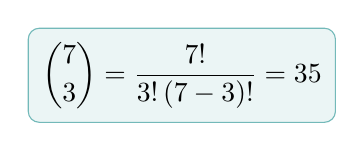
\begin{tikzpicture}
\node[draw=teal!55,rounded corners,fill=teal!8,inner sep=5pt] {$\displaystyle \binom{7}{3} = \frac{7!}{3!\,(7-3)!} = 35$};
\end{tikzpicture}
}
\end{center}
\small The binomial coefficient counts the ways to choose $r$ objects from $7$; large factorials cancel.\normalsize

\medskip\hrule

\section*{Binomial Expansion 09\quad\small\texttt{(be-009)}}
\addcontentsline{toc}{section}{Binomial Expansion 09 (be-009)}
\textit{Difficulty: Foundation \quad\textbar\quad Marks: 2}

\question{Without using a calculator, evaluate \( \binom{9}{2} \).}

\textbf{Worked solution.}

\textit{Step 1: Use the formula \(\binom{n}{r} = \frac{n!}{r!(n-r)!}\).}
\[\begin{gathered}
\binom{9}{2} = \frac{9!}{2! \times 7!} = \frac{9 \times 8}{2 \times 1}
\end{gathered}\]
Apply the formula.

\textit{Step 2: Simplify.}
\[\begin{gathered}
= \frac{72}{2} = 36
\end{gathered}\]
Simplify.

\begin{answerbox}
\textbf{Final answer:}\quad \(\displaystyle \binom{9}{2} = 36\)
\end{answerbox}
\textbf{Diagram.}

\begin{center}
\resizebox{\ifdim\width>\linewidth \linewidth\else \width\fi}{!}{%
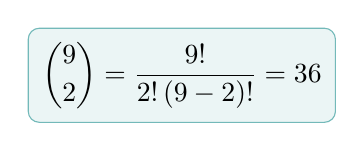
\begin{tikzpicture}
\node[draw=teal!55,rounded corners,fill=teal!8,inner sep=5pt] {$\displaystyle \binom{9}{2} = \frac{9!}{2!\,(9-2)!} = 36$};
\end{tikzpicture}
}
\end{center}
\small The binomial coefficient counts the ways to choose $r$ objects from $9$; large factorials cancel.\normalsize

\medskip\hrule

\section*{Binomial Expansion 10\quad\small\texttt{(be-010)}}
\addcontentsline{toc}{section}{Binomial Expansion 10 (be-010)}
\textit{Difficulty: Foundation \quad\textbar\quad Marks: 2}

\question{Without using a calculator, evaluate \( \binom{10}{4} \).}

\textbf{Worked solution.}

\textit{Step 1: Use the formula \(\binom{n}{r} = \frac{n!}{r!(n-r)!}\).}
\[\begin{gathered}
\binom{10}{4} = \frac{10 \times 9 \times 8 \times 7}{4 \times 3 \times 2 \times 1}
\end{gathered}\]
Apply the formula.

\textit{Step 2: Evaluate each term.}
\[\begin{gathered}
= \frac{5040}{24} = 210
\end{gathered}\]
Compute numerator and denominator.

\begin{answerbox}
\textbf{Final answer:}\quad \(\displaystyle \binom{10}{4} = 210\)
\end{answerbox}
\textbf{Diagram.}

\begin{center}
\resizebox{\ifdim\width>\linewidth \linewidth\else \width\fi}{!}{%
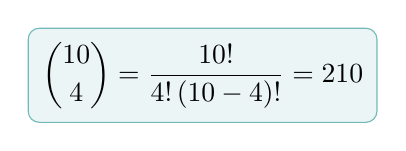
\begin{tikzpicture}
\node[draw=teal!55,rounded corners,fill=teal!8,inner sep=5pt] {$\displaystyle \binom{10}{4} = \frac{10!}{4!\,(10-4)!} = 210$};
\end{tikzpicture}
}
\end{center}
\small The binomial coefficient counts the ways to choose $r$ objects from $10$; large factorials cancel.\normalsize

\medskip\hrule

\section*{Binomial Expansion 11\quad\small\texttt{(be-011)}}
\addcontentsline{toc}{section}{Binomial Expansion 11 (be-011)}
\textit{Difficulty: Foundation \quad\textbar\quad Marks: 2}

\question{Without using a calculator, evaluate \( \binom{8}{5} \).}

\textbf{Worked solution.}

\textit{Use the formula \(\binom{n}{r} = \frac{n!}{r!(n-r)!}\).}
\[\begin{gathered}
\binom{8}{3} = \frac{8 \times 7 \times 6}{3 \times 2 \times 1} = \frac{336}{6} = 56
\end{gathered}\]
Use the symmetry property: \( \binom{8}{5} = \binom{8}{3} \).

\begin{answerbox}
\textbf{Final answer:}\quad \(\displaystyle \binom{8}{5} = 56\)
\end{answerbox}
\textbf{Diagram.}

\begin{center}
\resizebox{\ifdim\width>\linewidth \linewidth\else \width\fi}{!}{%
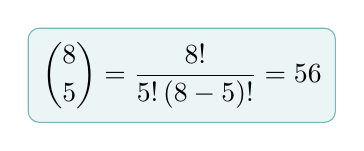
\begin{tikzpicture}
\node[draw=teal!55,rounded corners,fill=teal!8,inner sep=5pt] {$\displaystyle \binom{8}{5} = \frac{8!}{5!\,(8-5)!} = 56$};
\end{tikzpicture}
}
\end{center}
\small The binomial coefficient counts the ways to choose $r$ objects from $8$; large factorials cancel.\normalsize

\medskip\hrule

\section*{Binomial Expansion 12\quad\small\texttt{(be-012)}}
\addcontentsline{toc}{section}{Binomial Expansion 12 (be-012)}
\textit{Difficulty: Foundation \quad\textbar\quad Marks: 2}

\question{Evaluate \( \binom{12}{3} \) without a calculator.}

\textbf{Worked solution.}

\textit{Use the formula \(\binom{n}{r} = \frac{n!}{r!(n-r)!}\).}
\[\begin{gathered}
\binom{12}{3} = \frac{12 \times 11 \times 10}{3 \times 2 \times 1} = \frac{1320}{6} = 220
\end{gathered}\]
Apply the formula.

\begin{answerbox}
\textbf{Final answer:}\quad \(\displaystyle \binom{12}{3} = 220\)
\end{answerbox}
\textbf{Diagram.}

\begin{center}
\resizebox{\ifdim\width>\linewidth \linewidth\else \width\fi}{!}{%
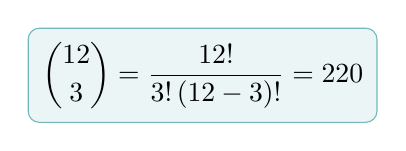
\begin{tikzpicture}
\node[draw=teal!55,rounded corners,fill=teal!8,inner sep=5pt] {$\displaystyle \binom{12}{3} = \frac{12!}{3!\,(12-3)!} = 220$};
\end{tikzpicture}
}
\end{center}
\small The binomial coefficient counts the ways to choose $r$ objects from $12$; large factorials cancel.\normalsize

\medskip\hrule

\section*{Binomial Expansion 13\quad\small\texttt{(be-013)}}
\addcontentsline{toc}{section}{Binomial Expansion 13 (be-013)}
\textit{Difficulty: Foundation \quad\textbar\quad Marks: 2}

\question{Find the value of \( \binom{n}{2} \) when \( n = 6 \).}

\textbf{Worked solution.}

\textit{Use the formula \(\binom{n}{r} = \frac{n!}{r!(n-r)!}\).}
\[\begin{gathered}
\binom{6}{2} = \frac{6 \times 5}{2 \times 1} = \frac{30}{2} = 15
\end{gathered}\]
Substitute \(n = 6\) into the formula.

\begin{answerbox}
\textbf{Final answer:}\quad \(\displaystyle \binom{6}{2} = 15\)
\end{answerbox}
\textbf{Diagram.}

\begin{center}
\resizebox{\ifdim\width>\linewidth \linewidth\else \width\fi}{!}{%
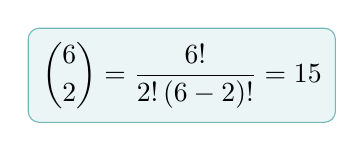
\begin{tikzpicture}
\node[draw=teal!55,rounded corners,fill=teal!8,inner sep=5pt] {$\displaystyle \binom{6}{2} = \frac{6!}{2!\,(6-2)!} = 15$};
\end{tikzpicture}
}
\end{center}
\small The binomial coefficient counts the ways to choose $r$ objects from $6$; large factorials cancel.\normalsize

\medskip\hrule

\section*{Binomial Expansion 14\quad\small\texttt{(be-014)}}
\addcontentsline{toc}{section}{Binomial Expansion 14 (be-014)}
\textit{Difficulty: Foundation \quad\textbar\quad Marks: 3}

\question{Evaluate \( \binom{11}{4} \) without a calculator, showing all working.}

\textbf{Worked solution.}

\textit{Step 1: Use the formula \(\binom{n}{r} = \frac{n!}{r!(n-r)!}\).}
\[\begin{gathered}
\binom{11}{4} = \frac{11!}{4! \times 7!} = \frac{11 \times 10 \times 9 \times 8}{4 \times 3 \times 2 \times 1}
\end{gathered}\]
Write out the formula.

\textit{Step 2: Evaluate each term.}
\[\begin{gathered}
\binom{11}{4} = \frac{7920}{24} = 330
\end{gathered}\]
Compute numerator: \(11 \times 10 = 110\), \(110 \times 9 = 990\), \(990 \times 8 = 7920\). Denominator: \(4! = 24\).

\begin{answerbox}
\textbf{Final answer:}\quad \(\displaystyle \binom{11}{4} = 330\)
\end{answerbox}
\textbf{Diagram.}

\begin{center}
\resizebox{\ifdim\width>\linewidth \linewidth\else \width\fi}{!}{%
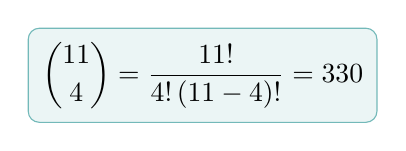
\begin{tikzpicture}
\node[draw=teal!55,rounded corners,fill=teal!8,inner sep=5pt] {$\displaystyle \binom{11}{4} = \frac{11!}{4!\,(11-4)!} = 330$};
\end{tikzpicture}
}
\end{center}
\small The binomial coefficient counts the ways to choose $r$ objects from $11$; large factorials cancel.\normalsize

\medskip\hrule

\section*{Binomial Expansion 15\quad\small\texttt{(be-015)}}
\addcontentsline{toc}{section}{Binomial Expansion 15 (be-015)}
\textit{Difficulty: Foundation \quad\textbar\quad Marks: 2}

\question{Find the coefficient of \( x^3 \) in the expansion of \( (1 + x)^8 \).}

\textbf{Worked solution.}

\textit{Use the binomial theorem to identify the general term.}
\[\begin{gathered}
\text{Coefficient of } x^3 = \binom{8}{3} = \frac{8 \times 7 \times 6}{3!} = \frac{336}{6} = 56
\end{gathered}\]
By the binomial theorem, \((1+x)^n = \sum_{r=0}^{n} \binom{n}{r} x^r\). The general term is \(\binom{n}{r} x^r\). To find the coefficient of \(x^3\), set \(r = 3\).

\begin{answerbox}
\textbf{Final answer:}\quad \(\displaystyle 56\)
\end{answerbox}
\textbf{Diagram.}

\begin{center}
\resizebox{\ifdim\width>\linewidth \linewidth\else \width\fi}{!}{%
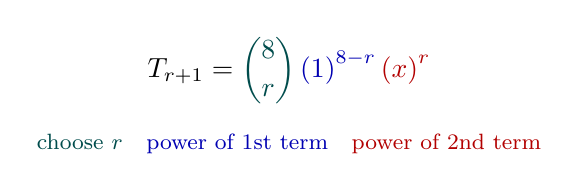
\begin{tikzpicture}
\node (T) {$\displaystyle T_{r+1} = {\color{teal!60!black}\binom{8}{r}}\,{\color{blue!70!black}\left(1\right)^{8-r}}\,{\color{red!70!black}\left(x\right)^{r}}$};
\node[below=4pt of T,font=\footnotesize] {{\color{teal!60!black}choose $r$}\quad{\color{blue!70!black}power of 1st term}\quad{\color{red!70!black}power of 2nd term}};
\end{tikzpicture}
}
\end{center}
\small General term of $\left(1+x\right)^{8}$. Set the power of $x$ to the required value to find $r$, then evaluate.\normalsize

\medskip\hrule

\section*{Binomial Expansion 16\quad\small\texttt{(be-016)}}
\addcontentsline{toc}{section}{Binomial Expansion 16 (be-016)}
\textit{Difficulty: Foundation \quad\textbar\quad Marks: 3}

\question{Find the coefficient of \( x^4 \) in the expansion of \( (1 - x)^{10} \).}

\textbf{Worked solution.}

\textit{Step 1: The general term of \((a+b)^n\) is \(\binom{n}{r} a^{n-r} b^r\). Identify the term with the required power.}
\[\begin{gathered}
\text{Term} = \binom{10}{4}(-1)^4 x^4 = 210 \times 1 \times x^4
\end{gathered}\]
The general term is \( \binom{10}{r}(-x)^r = \binom{10}{r}(-1)^r x^r \). For \(x^4\), set \(r = 4\).

\textit{Step 2: Simplify each term.}
\[\begin{gathered}
\text{Coefficient of } x^4 = 210
\end{gathered}\]
The coefficient is therefore \(+210\).

\begin{answerbox}
\textbf{Final answer:}\quad \(\displaystyle 210\)
\end{answerbox}
\textbf{Diagram.}

\begin{center}
\resizebox{\ifdim\width>\linewidth \linewidth\else \width\fi}{!}{%
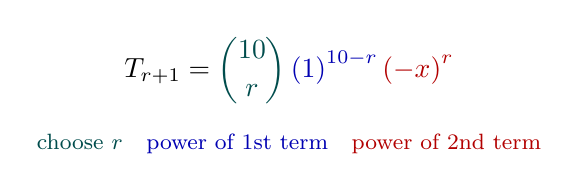
\begin{tikzpicture}
\node (T) {$\displaystyle T_{r+1} = {\color{teal!60!black}\binom{10}{r}}\,{\color{blue!70!black}\left(1\right)^{10-r}}\,{\color{red!70!black}\left(-x\right)^{r}}$};
\node[below=4pt of T,font=\footnotesize] {{\color{teal!60!black}choose $r$}\quad{\color{blue!70!black}power of 1st term}\quad{\color{red!70!black}power of 2nd term}};
\end{tikzpicture}
}
\end{center}
\small General term of $\left(1+-x\right)^{10}$. Set the power of $x$ to the required value to find $r$, then evaluate.\normalsize

\medskip\hrule

\section*{Binomial Expansion 17\quad\small\texttt{(be-017)}}
\addcontentsline{toc}{section}{Binomial Expansion 17 (be-017)}
\textit{Difficulty: Foundation \quad\textbar\quad Marks: 3}

\question{Find the coefficient of \( x^2 \) in the expansion of \( (1 + 3x)^{11} \).}

\textbf{Worked solution.}

\textit{The general term of \((a+b)^n\) is \(\binom{n}{r} a^{n-r} b^r\). Identify the term with the required power.}
\[\begin{gathered}
\text{Term} = \binom{11}{2}(3x)^2 = 55 \times 9x^2 = 495x^2
\end{gathered}\]
General term: \( \binom{11}{r}(3x)^r \). For \(x^2\), set \(r = 2\).

\begin{answerbox}
\textbf{Final answer:}\quad \(\displaystyle 495\)
\end{answerbox}
\textbf{Diagram.}

\begin{center}
\resizebox{\ifdim\width>\linewidth \linewidth\else \width\fi}{!}{%
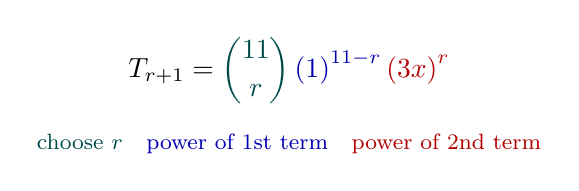
\begin{tikzpicture}
\node (T) {$\displaystyle T_{r+1} = {\color{teal!60!black}\binom{11}{r}}\,{\color{blue!70!black}\left(1\right)^{11-r}}\,{\color{red!70!black}\left(3x\right)^{r}}$};
\node[below=4pt of T,font=\footnotesize] {{\color{teal!60!black}choose $r$}\quad{\color{blue!70!black}power of 1st term}\quad{\color{red!70!black}power of 2nd term}};
\end{tikzpicture}
}
\end{center}
\small General term of $\left(1+3x\right)^{11}$. Set the power of $x$ to the required value to find $r$, then evaluate.\normalsize

\medskip\hrule

\section*{Binomial Expansion 18\quad\small\texttt{(be-018)}}
\addcontentsline{toc}{section}{Binomial Expansion 18 (be-018)}
\textit{Difficulty: Foundation \quad\textbar\quad Marks: 3}

\question{Find the coefficient of \( x^3 \) in the expansion of \( (1 - 2x)^9 \).}

\textbf{Worked solution.}

\textit{The general term of \((a+b)^n\) is \(\binom{n}{r} a^{n-r} b^r\). Identify the term with the required power.}
\[\begin{gathered}
\text{Term} = \binom{9}{3}(-2)^3 x^3 = 84 \times (-8) x^3 = -672x^3
\end{gathered}\]
General term: \( \binom{9}{r}(-2x)^r \). For \(x^3\), set \(r = 3\).

\begin{answerbox}
\textbf{Final answer:}\quad \(\displaystyle -672\)
\end{answerbox}
\textbf{Diagram.}

\begin{center}
\resizebox{\ifdim\width>\linewidth \linewidth\else \width\fi}{!}{%
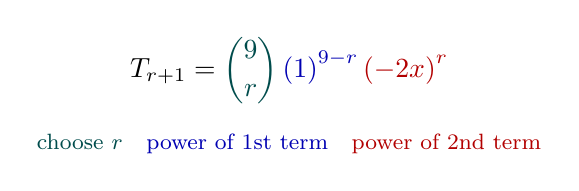
\begin{tikzpicture}
\node (T) {$\displaystyle T_{r+1} = {\color{teal!60!black}\binom{9}{r}}\,{\color{blue!70!black}\left(1\right)^{9-r}}\,{\color{red!70!black}\left(-2x\right)^{r}}$};
\node[below=4pt of T,font=\footnotesize] {{\color{teal!60!black}choose $r$}\quad{\color{blue!70!black}power of 1st term}\quad{\color{red!70!black}power of 2nd term}};
\end{tikzpicture}
}
\end{center}
\small General term of $\left(1+-2x\right)^{9}$. Set the power of $x$ to the required value to find $r$, then evaluate.\normalsize

\medskip\hrule

\section*{Binomial Expansion 19\quad\small\texttt{(be-019)}}
\addcontentsline{toc}{section}{Binomial Expansion 19 (be-019)}
\textit{Difficulty: Foundation \quad\textbar\quad Marks: 3}

\question{Find the coefficient of \( x^2 \) in the expansion of \( (2 + x)^6 \).}

\textbf{Worked solution.}

\textit{The general term of \((a+b)^n\) is \(\binom{n}{r} a^{n-r} b^r\). Identify the term with the required power.}
\[\begin{gathered}
\text{Term} = \binom{6}{2}(2)^4 x^2 = 15 \times 16 \times x^2 = 240x^2
\end{gathered}\]
General term: \( \binom{6}{r}(2)^{6-r} x^r \). For \(x^2\), set \(r = 2\).

\begin{answerbox}
\textbf{Final answer:}\quad \(\displaystyle 240\)
\end{answerbox}
\textbf{Diagram.}

\begin{center}
\resizebox{\ifdim\width>\linewidth \linewidth\else \width\fi}{!}{%
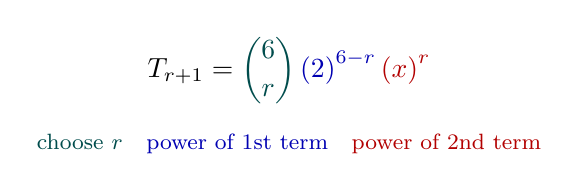
\begin{tikzpicture}
\node (T) {$\displaystyle T_{r+1} = {\color{teal!60!black}\binom{6}{r}}\,{\color{blue!70!black}\left(2\right)^{6-r}}\,{\color{red!70!black}\left(x\right)^{r}}$};
\node[below=4pt of T,font=\footnotesize] {{\color{teal!60!black}choose $r$}\quad{\color{blue!70!black}power of 1st term}\quad{\color{red!70!black}power of 2nd term}};
\end{tikzpicture}
}
\end{center}
\small General term of $\left(2+x\right)^{6}$. Set the power of $x$ to the required value to find $r$, then evaluate.\normalsize

\medskip\hrule

\section*{Binomial Expansion 20\quad\small\texttt{(be-020)}}
\addcontentsline{toc}{section}{Binomial Expansion 20 (be-020)}
\textit{Difficulty: Foundation \quad\textbar\quad Marks: 3}

\question{Find the coefficient of \( x^3 \) in the expansion of \( (3 + 2x)^5 \).}

\textbf{Worked solution.}

\textit{The general term of \((a+b)^n\) is \(\binom{n}{r} a^{n-r} b^r\). Identify the term with the required power.}
\[\begin{gathered}
\text{Term} = \binom{5}{3}(3)^2(2)^3 x^3 = 10 \times 9 \times 8 \times x^3 = 720x^3
\end{gathered}\]
General term: \( \binom{5}{r}(3)^{5-r}(2x)^r \). For \(x^3\), set \(r = 3\).

\begin{answerbox}
\textbf{Final answer:}\quad \(\displaystyle 720\)
\end{answerbox}
\textbf{Diagram.}

\begin{center}
\resizebox{\ifdim\width>\linewidth \linewidth\else \width\fi}{!}{%
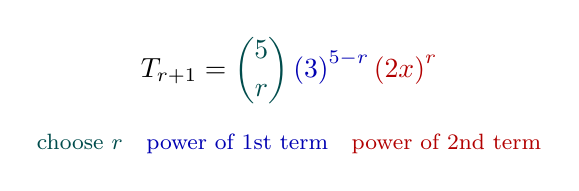
\begin{tikzpicture}
\node (T) {$\displaystyle T_{r+1} = {\color{teal!60!black}\binom{5}{r}}\,{\color{blue!70!black}\left(3\right)^{5-r}}\,{\color{red!70!black}\left(2x\right)^{r}}$};
\node[below=4pt of T,font=\footnotesize] {{\color{teal!60!black}choose $r$}\quad{\color{blue!70!black}power of 1st term}\quad{\color{red!70!black}power of 2nd term}};
\end{tikzpicture}
}
\end{center}
\small General term of $\left(3+2x\right)^{5}$. Set the power of $x$ to the required value to find $r$, then evaluate.\normalsize

\medskip\hrule

\section*{Binomial Expansion 21\quad\small\texttt{(be-021)}}
\addcontentsline{toc}{section}{Binomial Expansion 21 (be-021)}
\textit{Difficulty: Foundation \quad\textbar\quad Marks: 2}

\question{Find the coefficient of \( x^5 \) in the expansion of \( (1 + x)^7 \).}

\textbf{Worked solution.}

\textit{The general term of \((a+b)^n\) is \(\binom{n}{r} a^{n-r} b^r\). Identify the term with the required power.}
\[\begin{gathered}
\binom{7}{2} = \frac{7 \times 6}{2} = 21
\end{gathered}\]
General term: \( \binom{7}{r} x^r \). For \(x^5\), set \(r = 5\). Use symmetry: \( \binom{7}{5} = \binom{7}{2} \).

\begin{answerbox}
\textbf{Final answer:}\quad \(\displaystyle 21\)
\end{answerbox}
\textbf{Diagram.}

\begin{center}
\resizebox{\ifdim\width>\linewidth \linewidth\else \width\fi}{!}{%
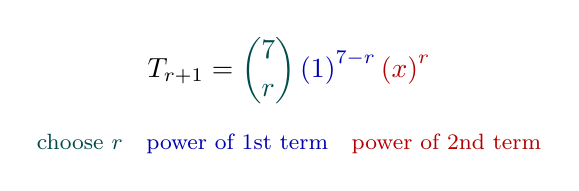
\begin{tikzpicture}
\node (T) {$\displaystyle T_{r+1} = {\color{teal!60!black}\binom{7}{r}}\,{\color{blue!70!black}\left(1\right)^{7-r}}\,{\color{red!70!black}\left(x\right)^{r}}$};
\node[below=4pt of T,font=\footnotesize] {{\color{teal!60!black}choose $r$}\quad{\color{blue!70!black}power of 1st term}\quad{\color{red!70!black}power of 2nd term}};
\end{tikzpicture}
}
\end{center}
\small General term of $\left(1+x\right)^{7}$. Set the power of $x$ to the required value to find $r$, then evaluate.\normalsize

\medskip\hrule

\section*{Binomial Expansion 22\quad\small\texttt{(be-022)}}
\addcontentsline{toc}{section}{Binomial Expansion 22 (be-022)}
\textit{Difficulty: Foundation \quad\textbar\quad Marks: 4}

\question{The expansion of \( (1 + ax)^6 \) has coefficient of \( x^2 \) equal to 60. Find the value of \( a \).}

\textbf{Worked solution.}

\textit{Step 1: The general term of \((a+b)^n\) is \(\binom{n}{r} a^{n-r} b^r\). Identify the term with the required power.}
\[\begin{gathered}
\binom{6}{2} a^2 = 15a^2
\end{gathered}\]
The coefficient of \(x^2\) in \((1+ax)^6\) is \( \binom{6}{2} a^2 \).

\textit{Step 2: Set the power of \(x\) to zero.}
\[\begin{gathered}
15a^2 = 60 \implies a^2 = 4 \implies a = \pm 2
\end{gathered}\]
Set this equal to 60 and solve.

\begin{answerbox}
\textbf{Final answer:}\quad \(\displaystyle a = 2 or a = -2\)
\end{answerbox}
\textbf{Diagram.}

\begin{center}
\resizebox{\ifdim\width>\linewidth \linewidth\else \width\fi}{!}{%
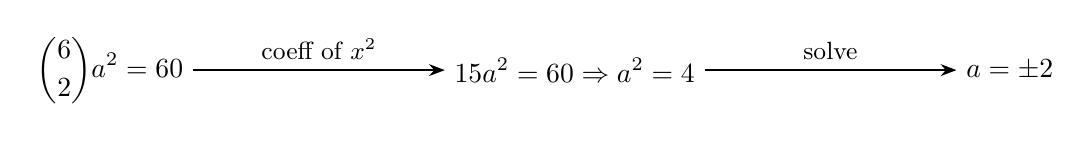
\begin{tikzpicture}[>={Stealth[length=2mm]},node distance=1.5cm and 3.2cm]
\node (s0) {$\displaystyle \binom{6}{2}a^{2}=60$};
\node (s1) [right=of s0] {$\displaystyle 15a^{2}=60\Rightarrow a^{2}=4$};
\node (s2) [right=of s1] {$\displaystyle a=\pm2$};
\draw[->,thick] (s0) -- (s1) node[midway,above,font=\small]{coeff of $x^{2}$};
\draw[->,thick] (s1) -- (s2) node[midway,above,font=\small]{solve};
\end{tikzpicture}
}
\end{center}
\small Solution flow: each arrow applies one step.\normalsize

\medskip\hrule

\section*{Binomial Expansion 23\quad\small\texttt{(be-023)}}
\addcontentsline{toc}{section}{Binomial Expansion 23 (be-023)}
\textit{Difficulty: Foundation \quad\textbar\quad Marks: 4}

\question{Find the term independent of \( x \) in the expansion of \( \left(x - \dfrac{1}{x}\right)^6 \).}

\textbf{Worked solution.}

\textit{Step 1: Write the general term using the binomial theorem.}
\[\begin{gathered}
T_{r+1} = \binom{6}{r}(x)^{6-r}\left(-\frac{1}{x}\right)^r = \binom{6}{r}(-1)^r x^{6-2r}
\end{gathered}\]
By the binomial theorem, \((a+b)^n = \sum_{r=0}^{n} \binom{n}{r} a^{n-r} b^r\). Here \(a = x\), \(b = -\frac{1}{x}\), \(n = 6\). Combine the powers of \(x\) into a single exponent.

\textit{Step 2: Set the power of \(x\) to zero to find the term independent of \(x\).}
\[\begin{gathered}
6 - 2r = 0 \quad\quad \Rightarrow \quad\quad r = 3
\end{gathered}\]
The term independent of \(x\) is the term where the exponent of \(x\) equals zero.

\textit{Step 3: Substitute \(r = 3\) into the general term.}
\[\begin{gathered}
T_4 = \binom{6}{3}(-1)^3 = 20 \times (-1) = -20
\end{gathered}\]
\begin{answerbox}
\textbf{Final answer:}\quad \(\displaystyle -20\)
\end{answerbox}
\textbf{Diagram.}

\begin{center}
\resizebox{\ifdim\width>\linewidth \linewidth\else \width\fi}{!}{%
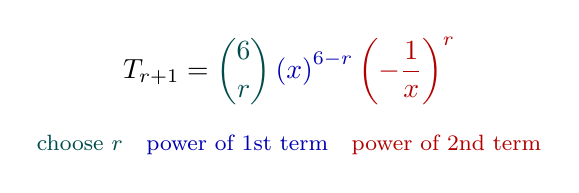
\begin{tikzpicture}
\node (T) {$\displaystyle T_{r+1} = {\color{teal!60!black}\binom{6}{r}}\,{\color{blue!70!black}\left(x\right)^{6-r}}\,{\color{red!70!black}\left(-\frac{1}{x}\right)^{r}}$};
\node[below=4pt of T,font=\footnotesize] {{\color{teal!60!black}choose $r$}\quad{\color{blue!70!black}power of 1st term}\quad{\color{red!70!black}power of 2nd term}};
\end{tikzpicture}
}
\end{center}
\small General term of $\left(x+-\frac{1}{x}\right)^{6}$. Set the power of $x$ to the required value to find $r$, then evaluate.\normalsize

\medskip\hrule

\section*{Binomial Expansion 24\quad\small\texttt{(be-024)}}
\addcontentsline{toc}{section}{Binomial Expansion 24 (be-024)}
\textit{Difficulty: Foundation \quad\textbar\quad Marks: 4}

\question{Find the term independent of \( x \) in the expansion of \( \left(x + \dfrac{2}{x}\right)^4 \).}

\textbf{Worked solution.}

\textit{Step 1: Write the general term using \((a+b)^n = \sum \binom{n}{r} a^{n-r} b^r\) and set the power of \(x\) to zero.}
\[\begin{gathered}
T_{r+1} = \binom{4}{r} 2^r x^{4-2r}
\end{gathered}\]
General term: \( \binom{4}{r}(x)^{4-r}\left(\dfrac{2}{x}\right)^r = \binom{4}{r} 2^r x^{4-r} x^{-r} = \binom{4}{r} 2^r x^{4-2r} \).

\textit{Step 2: Set the power of \(x\) to zero.}
\[\begin{gathered}
r = 2
\end{gathered}\]
Set \(4 - 2r = 0 \Rightarrow r = 2\).

\textit{Step 3: Substitute and evaluate.}
\[\begin{gathered}
T_3 = 24
\end{gathered}\]
Substitute: \(\binom{4}{2} \times 2^2 = 6 \times 4 = 24\).

\begin{answerbox}
\textbf{Final answer:}\quad \(\displaystyle 24\)
\end{answerbox}
\textbf{Diagram.}

\begin{center}
\resizebox{\ifdim\width>\linewidth \linewidth\else \width\fi}{!}{%
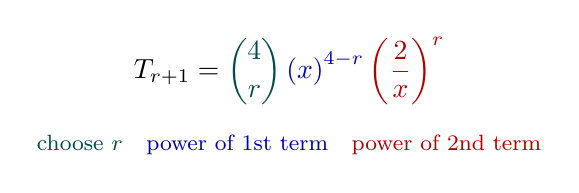
\begin{tikzpicture}
\node (T) {$\displaystyle T_{r+1} = {\color{teal!60!black}\binom{4}{r}}\,{\color{blue!70!black}\left(x\right)^{4-r}}\,{\color{red!70!black}\left(\frac{2}{x}\right)^{r}}$};
\node[below=4pt of T,font=\footnotesize] {{\color{teal!60!black}choose $r$}\quad{\color{blue!70!black}power of 1st term}\quad{\color{red!70!black}power of 2nd term}};
\end{tikzpicture}
}
\end{center}
\small General term of $\left(x+\frac{2}{x}\right)^{4}$. Set the power of $x$ to the required value to find $r$, then evaluate.\normalsize

\medskip\hrule

\section*{Binomial Expansion 25\quad\small\texttt{(be-025)}}
\addcontentsline{toc}{section}{Binomial Expansion 25 (be-025)}
\textit{Difficulty: Foundation \quad\textbar\quad Marks: 5}

\question{Find the term independent of \( x \) in the expansion of \( \left(2x - \dfrac{1}{x^2}\right)^6 \).}

\textbf{Worked solution.}

\textit{Step 1: Write the general term using \((a+b)^n = \sum \binom{n}{r} a^{n-r} b^r\) and set the power of \(x\) to zero.}
\[\begin{gathered}
T_{r+1} = \binom{6}{r} 2^{6-r}(-1)^r x^{6-3r}
\end{gathered}\]
General term: \( \binom{6}{r}(2x)^{6-r}\left(-\dfrac{1}{x^2}\right)^r = \binom{6}{r} 2^{6-r}(-1)^r x^{6-r} \cdot x^{-2r} \).

\textit{Step 2: Find the required term.}
\[\begin{gathered}
r = 2
\end{gathered}\]
For independence from \(x\): \(6 - 3r = 0 \Rightarrow r = 2\).

\textit{Step 3: Substitute and evaluate.}
\[\begin{gathered}
T_3 = 240
\end{gathered}\]
Substitute: \(\binom{6}{2} \times 2^4 \times (-1)^2 = 15 \times 16 \times 1 = 240\).

\begin{answerbox}
\textbf{Final answer:}\quad \(\displaystyle 240\)
\end{answerbox}
\textbf{Diagram.}

\begin{center}
\resizebox{\ifdim\width>\linewidth \linewidth\else \width\fi}{!}{%
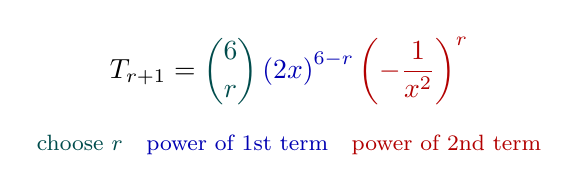
\begin{tikzpicture}
\node (T) {$\displaystyle T_{r+1} = {\color{teal!60!black}\binom{6}{r}}\,{\color{blue!70!black}\left(2x\right)^{6-r}}\,{\color{red!70!black}\left(-\frac{1}{x^{2}}\right)^{r}}$};
\node[below=4pt of T,font=\footnotesize] {{\color{teal!60!black}choose $r$}\quad{\color{blue!70!black}power of 1st term}\quad{\color{red!70!black}power of 2nd term}};
\end{tikzpicture}
}
\end{center}
\small General term of $\left(2x+-\frac{1}{x^{2}}\right)^{6}$. Set the power of $x$ to the required value to find $r$, then evaluate.\normalsize

\medskip\hrule

\section*{Binomial Expansion 26\quad\small\texttt{(be-026)}}
\addcontentsline{toc}{section}{Binomial Expansion 26 (be-026)}
\textit{Difficulty: Foundation \quad\textbar\quad Marks: 4}

\question{Find the term independent of \( x \) in the expansion of \( \left(x^2 + \dfrac{1}{x}\right)^6 \).}

\textbf{Worked solution.}

\textit{Step 1: Write the general term using \((a+b)^n = \sum \binom{n}{r} a^{n-r} b^r\) and set the power of \(x\) to zero.}
\[\begin{gathered}
T_{r+1} = \binom{6}{r} x^{12-3r}
\end{gathered}\]
General term: \( \binom{6}{r}(x^2)^{6-r}\left(\dfrac{1}{x}\right)^r = \binom{6}{r} x^{12-2r} \cdot x^{-r} = \binom{6}{r} x^{12-3r} \).

\textit{Step 2: Set the power of \(x\) to zero.}
\[\begin{gathered}
r = 4
\end{gathered}\]
Set \(12 - 3r = 0 \Rightarrow r = 4\).

\textit{Step 3: Substitute and evaluate.}
\[\begin{gathered}
T_5 = 15
\end{gathered}\]
Substitute: \(\binom{6}{4} = \binom{6}{2} = 15\).

\begin{answerbox}
\textbf{Final answer:}\quad \(\displaystyle 15\)
\end{answerbox}
\textbf{Diagram.}

\begin{center}
\resizebox{\ifdim\width>\linewidth \linewidth\else \width\fi}{!}{%
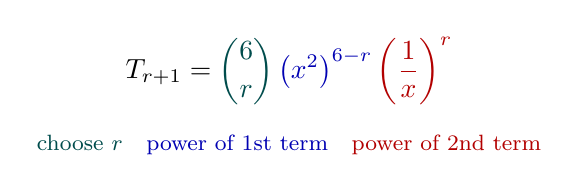
\begin{tikzpicture}
\node (T) {$\displaystyle T_{r+1} = {\color{teal!60!black}\binom{6}{r}}\,{\color{blue!70!black}\left(x^{2}\right)^{6-r}}\,{\color{red!70!black}\left(\frac{1}{x}\right)^{r}}$};
\node[below=4pt of T,font=\footnotesize] {{\color{teal!60!black}choose $r$}\quad{\color{blue!70!black}power of 1st term}\quad{\color{red!70!black}power of 2nd term}};
\end{tikzpicture}
}
\end{center}
\small General term of $\left(x^{2}+\frac{1}{x}\right)^{6}$. Set the power of $x$ to the required value to find $r$, then evaluate.\normalsize

\medskip\hrule

\section*{Binomial Expansion 27\quad\small\texttt{(be-027)}}
\addcontentsline{toc}{section}{Binomial Expansion 27 (be-027)}
\textit{Difficulty: Foundation \quad\textbar\quad Marks: 5}

\question{Find the term independent of \( x \) in the expansion of \( \left(x - \dfrac{3}{x}\right)^8 \).}

\textbf{Worked solution.}

\textit{Step 1: Write the general term using \((a+b)^n = \sum \binom{n}{r} a^{n-r} b^r\) and set the power of \(x\) to zero.}
\[\begin{gathered}
T_{r+1} = \binom{8}{r}(-3)^r x^{8-2r}
\end{gathered}\]
General term: \( \binom{8}{r}(x)^{8-r}\left(-\dfrac{3}{x}\right)^r = \binom{8}{r}(-3)^r x^{8-2r} \).

\textit{Step 2: Set the power of \(x\) to zero.}
\[\begin{gathered}
r = 4
\end{gathered}\]
Set \(8 - 2r = 0 \Rightarrow r = 4\).

\textit{Step 3: Substitute and evaluate.}
\[\begin{gathered}
T_5 = 5670
\end{gathered}\]
Substitute: \(\binom{8}{4} \times (-3)^4 = 70 \times 81 = 5670\).

\begin{answerbox}
\textbf{Final answer:}\quad \(\displaystyle 5670\)
\end{answerbox}
\textbf{Diagram.}

\begin{center}
\resizebox{\ifdim\width>\linewidth \linewidth\else \width\fi}{!}{%
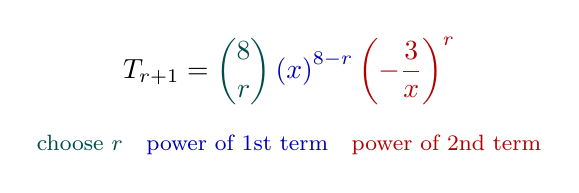
\begin{tikzpicture}
\node (T) {$\displaystyle T_{r+1} = {\color{teal!60!black}\binom{8}{r}}\,{\color{blue!70!black}\left(x\right)^{8-r}}\,{\color{red!70!black}\left(-\frac{3}{x}\right)^{r}}$};
\node[below=4pt of T,font=\footnotesize] {{\color{teal!60!black}choose $r$}\quad{\color{blue!70!black}power of 1st term}\quad{\color{red!70!black}power of 2nd term}};
\end{tikzpicture}
}
\end{center}
\small General term of $\left(x+-\frac{3}{x}\right)^{8}$. Set the power of $x$ to the required value to find $r$, then evaluate.\normalsize

\medskip\hrule

\section*{Binomial Expansion 28\quad\small\texttt{(be-028)}}
\addcontentsline{toc}{section}{Binomial Expansion 28 (be-028)}
\textit{Difficulty: Foundation \quad\textbar\quad Marks: 5}

\question{Find the term independent of \( x \) in the expansion of \( \left(3x + \dfrac{1}{x^2}\right)^9 \).}

\textbf{Worked solution.}

\textit{Step 1: Write the general term using \((a+b)^n = \sum \binom{n}{r} a^{n-r} b^r\) and set the power of \(x\) to zero.}
\[\begin{gathered}
T_{r+1} = \binom{9}{r} 3^{9-r} x^{9-3r}
\end{gathered}\]
General term: \( \binom{9}{r}(3x)^{9-r}\left(\dfrac{1}{x^2}\right)^r = \binom{9}{r} 3^{9-r} x^{9-r} x^{-2r} = \binom{9}{r} 3^{9-r} x^{9-3r} \).

\textit{Step 2: Set the power of \(x\) to zero.}
\[\begin{gathered}
r = 3
\end{gathered}\]
Set \(9 - 3r = 0 \Rightarrow r = 3\).

\textit{Step 3: Substitute and evaluate.}
\[\begin{gathered}
T_4 = 61236
\end{gathered}\]
Substitute: \(\binom{9}{3} \times 3^6 = 84 \times 729 = 61236\).

\begin{answerbox}
\textbf{Final answer:}\quad \(\displaystyle 61236\)
\end{answerbox}
\textbf{Diagram.}

\begin{center}
\resizebox{\ifdim\width>\linewidth \linewidth\else \width\fi}{!}{%
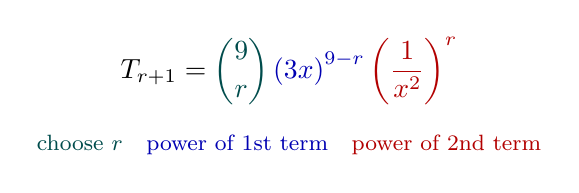
\begin{tikzpicture}
\node (T) {$\displaystyle T_{r+1} = {\color{teal!60!black}\binom{9}{r}}\,{\color{blue!70!black}\left(3x\right)^{9-r}}\,{\color{red!70!black}\left(\frac{1}{x^{2}}\right)^{r}}$};
\node[below=4pt of T,font=\footnotesize] {{\color{teal!60!black}choose $r$}\quad{\color{blue!70!black}power of 1st term}\quad{\color{red!70!black}power of 2nd term}};
\end{tikzpicture}
}
\end{center}
\small General term of $\left(3x+\frac{1}{x^{2}}\right)^{9}$. Set the power of $x$ to the required value to find $r$, then evaluate.\normalsize

\medskip\hrule

\section*{Binomial Expansion 29\quad\small\texttt{(be-029)}}
\addcontentsline{toc}{section}{Binomial Expansion 29 (be-029)}
\textit{Difficulty: Foundation \quad\textbar\quad Marks: 7}

\question{(a) Write down the first three terms, in ascending powers of \( x \), of the expansion of \( (1 + x)^{10} \). \\[3pt] (b) Use your expansion with \( x = 0.01 \) to find an approximate value of \( 1.01^{10} \). \\[3pt] (c) Calculate the percentage error in your approximation compared to the exact value \( 1.01^{10} = 1.10462 \) (to 5 d.p.).}

\textbf{Worked solution.}

\textit{Step 1: Apply the binomial theorem: \((a+b)^n = \sum_{r=0}^{n} \binom{n}{r} a^{n-r} b^r\). Write the first few terms.}
\[\begin{gathered}
(1+x)^{10} \approx 1 + 10x + \binom{10}{2}x^2 = 1 + 10x + 45x^2
\end{gathered}\]
(a) The first three terms are:

\textit{Step 2: Simplify each term.}
\[\begin{gathered}
1 + 10(0.01) + 45(0.01)^2 = 1 + 0.1 + 45 \times 0.0001 = 1 + 0.1 + 0.0045 = 1.1045
\end{gathered}\]
(b) Substitute \(x = 0.01\):

\textit{Step 3: Collect and simplify.}
\[\begin{gathered}
\text{\% error} = \frac{|1.1045 - 1.10462|}{1.10462} \times 100 = \frac{0.00012}{1.10462} \times 100 \approx 0.011\%
\end{gathered}\]
(c) Percentage error:

\begin{answerbox}
\textbf{Final answer:}\quad \(\displaystyle (a) 1 + 10x + 45x^2; (b) 1.1045; (c) approximately 0.011\%\)
\end{answerbox}
\textbf{Diagram.}

\begin{center}
\resizebox{\ifdim\width>\linewidth \linewidth\else \width\fi}{!}{%
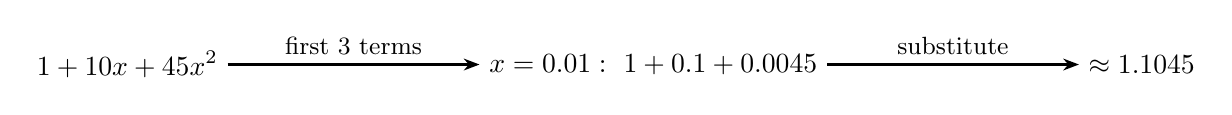
\begin{tikzpicture}[>={Stealth[length=2mm]},node distance=1.5cm and 3.2cm]
\node (s0) {$\displaystyle 1+10x+45x^{2}$};
\node (s1) [right=of s0] {$\displaystyle x=0.01:\ 1+0.1+0.0045$};
\node (s2) [right=of s1] {$\displaystyle \approx 1.1045$};
\draw[->,thick] (s0) -- (s1) node[midway,above,font=\small]{first 3 terms};
\draw[->,thick] (s1) -- (s2) node[midway,above,font=\small]{substitute};
\end{tikzpicture}
}
\end{center}
\small Solution flow: each arrow applies one step.\normalsize

\medskip\hrule

\section*{Binomial Expansion 30\quad\small\texttt{(be-030)}}
\addcontentsline{toc}{section}{Binomial Expansion 30 (be-030)}
\textit{Difficulty: Foundation \quad\textbar\quad Marks: 6}

\question{(a) Expand \( (2 - x)^5 \) in ascending powers of \( x \), up to and including the \( x^3 \) term. \\[3pt] (b) Use \( x = 0.1 \) to find an approximate value of \( 1.9^5 \).}

\textbf{Worked solution.}

\textit{Step 1: Apply the binomial theorem: \((a+b)^n = \sum_{r=0}^{n} \binom{n}{r} a^{n-r} b^r\).}
\[\begin{gathered}
(2-x)^5 = \binom{5}{0}2^5 + \binom{5}{1}2^4(-x) + \binom{5}{2}2^3(-x)^2 + \binom{5}{3}2^2(-x)^3 + \ldots
\end{gathered}\]
(a) Write out the first four terms with \(a=2\), \(b=-x\):

\textit{Step 2: Evaluate each term.}
\[\begin{gathered}
= 32 - 80x + 80x^2 - 40x^3 + \ldots
\end{gathered}\]
Compute each term:

\textit{Step 3: Collect and simplify.}
\[\begin{gathered}
1.9^5 \approx 32 - 80(0.1) + 80(0.01) - 40(0.001) = 32 - 8 + 0.8 - 0.04 = 24.76
\end{gathered}\]
(b) Substitute \(x = 0.1\):

\begin{answerbox}
\textbf{Final answer:}\quad \(\displaystyle (a) 32 - 80x + 80x^2 - 40x^3; (b) 1.9^5 \approx 24.76\)
\end{answerbox}
\textbf{Diagram.}

\begin{center}
\resizebox{\ifdim\width>\linewidth \linewidth\else \width\fi}{!}{%
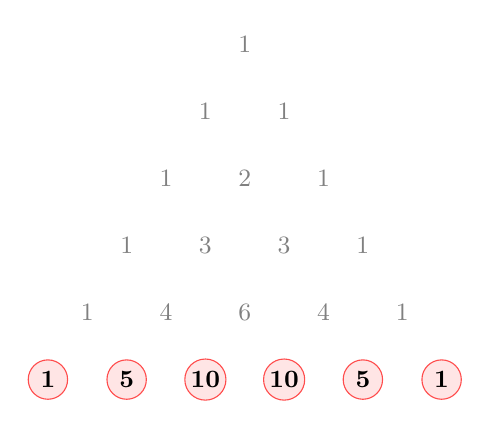
\begin{tikzpicture}[font=\small]
\node[gray] at (0,0) {$1$};
\node[gray] at (-0.5,-0.85) {$1$};
\node[gray] at (0.5,-0.85) {$1$};
\node[gray] at (-1,-1.7) {$1$};
\node[gray] at (0,-1.7) {$2$};
\node[gray] at (1,-1.7) {$1$};
\node[gray] at (-1.5,-2.55) {$1$};
\node[gray] at (-0.5,-2.55) {$3$};
\node[gray] at (0.5,-2.55) {$3$};
\node[gray] at (1.5,-2.55) {$1$};
\node[gray] at (-2,-3.4) {$1$};
\node[gray] at (-1,-3.4) {$4$};
\node[gray] at (0,-3.4) {$6$};
\node[gray] at (1,-3.4) {$4$};
\node[gray] at (2,-3.4) {$1$};
\node[circle,draw=red!70,fill=red!10,inner sep=1pt,minimum size=5mm] at (-2.5,-4.25) {$\mathbf{1}$};
\node[circle,draw=red!70,fill=red!10,inner sep=1pt,minimum size=5mm] at (-1.5,-4.25) {$\mathbf{5}$};
\node[circle,draw=red!70,fill=red!10,inner sep=1pt,minimum size=5mm] at (-0.5,-4.25) {$\mathbf{10}$};
\node[circle,draw=red!70,fill=red!10,inner sep=1pt,minimum size=5mm] at (0.5,-4.25) {$\mathbf{10}$};
\node[circle,draw=red!70,fill=red!10,inner sep=1pt,minimum size=5mm] at (1.5,-4.25) {$\mathbf{5}$};
\node[circle,draw=red!70,fill=red!10,inner sep=1pt,minimum size=5mm] at (2.5,-4.25) {$\mathbf{1}$};
\end{tikzpicture}
}
\end{center}
\small Row $5$ of Pascal's triangle (red) gives the binomial coefficients $\binom{5}{r}$; multiply each by the matching powers $a^{\,5-r}b^{\,r}$.\normalsize

\medskip\hrule

\section*{Binomial Expansion 31\quad\small\texttt{(be-031)}}
\addcontentsline{toc}{section}{Binomial Expansion 31 (be-031)}
\textit{Difficulty: Foundation \quad\textbar\quad Marks: 7}

\question{(a) Write down the first four terms, in ascending powers of \( x \), of the expansion of \( (1 - 3x)^7 \). \\[3pt] (b) Use your expansion with a suitable value of \( x \) to estimate \( 0.97^7 \), giving your answer to 4 decimal places.}

\textbf{Worked solution.}

\textit{Step 1: Apply the binomial theorem: \((a+b)^n = \sum_{r=0}^{n} \binom{n}{r} a^{n-r} b^r\). Write the first few terms.}
\[\begin{gathered}
(1-3x)^7 \approx 1 - 21x + 189x^2 - 945x^3 + \ldots
\end{gathered}\]
(a) The general term is \(\binom{7}{r}(-3x)^r\). Write the first four terms:

\textit{Step 2: Simplify each term.}
\[\begin{gathered}
0.97^7 \approx 1 - 21(0.01) + 189(0.0001) - 945(0.000001)
\end{gathered}\]
(b) We need \(0.97^7\). Set \(1 - 3x = 0.97 \Rightarrow x = 0.01\).

\textit{Step 3: Collect and simplify.}
\[\begin{gathered}
= 1 - 0.21 + 0.0189 - 0.000945 = 0.8080 \text{ (to 4 d.p.)}
\end{gathered}\]
Compute:

\begin{answerbox}
\textbf{Final answer:}\quad \(\displaystyle (a) 1 - 21x + 189x^2 - 945x^3 + \ldots; (b) 0.97^7 \approx 0.8080\)
\end{answerbox}
\textbf{Diagram.}

\begin{center}
\resizebox{\ifdim\width>\linewidth \linewidth\else \width\fi}{!}{%
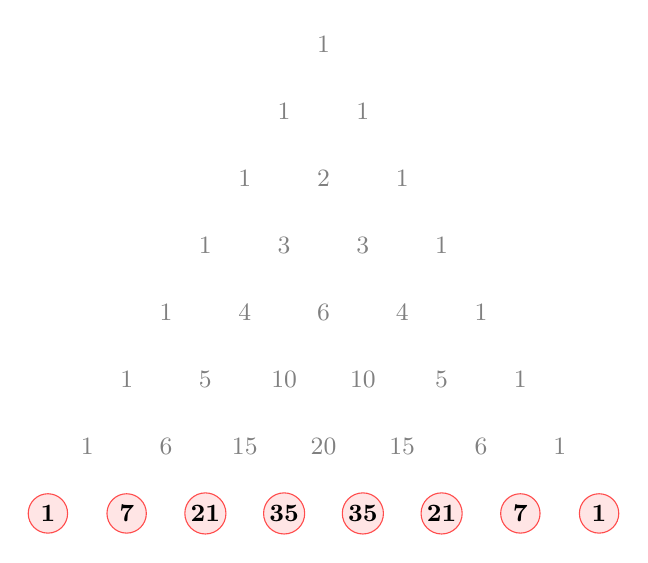
\begin{tikzpicture}[font=\small]
\node[gray] at (0,0) {$1$};
\node[gray] at (-0.5,-0.85) {$1$};
\node[gray] at (0.5,-0.85) {$1$};
\node[gray] at (-1,-1.7) {$1$};
\node[gray] at (0,-1.7) {$2$};
\node[gray] at (1,-1.7) {$1$};
\node[gray] at (-1.5,-2.55) {$1$};
\node[gray] at (-0.5,-2.55) {$3$};
\node[gray] at (0.5,-2.55) {$3$};
\node[gray] at (1.5,-2.55) {$1$};
\node[gray] at (-2,-3.4) {$1$};
\node[gray] at (-1,-3.4) {$4$};
\node[gray] at (0,-3.4) {$6$};
\node[gray] at (1,-3.4) {$4$};
\node[gray] at (2,-3.4) {$1$};
\node[gray] at (-2.5,-4.25) {$1$};
\node[gray] at (-1.5,-4.25) {$5$};
\node[gray] at (-0.5,-4.25) {$10$};
\node[gray] at (0.5,-4.25) {$10$};
\node[gray] at (1.5,-4.25) {$5$};
\node[gray] at (2.5,-4.25) {$1$};
\node[gray] at (-3,-5.1) {$1$};
\node[gray] at (-2,-5.1) {$6$};
\node[gray] at (-1,-5.1) {$15$};
\node[gray] at (0,-5.1) {$20$};
\node[gray] at (1,-5.1) {$15$};
\node[gray] at (2,-5.1) {$6$};
\node[gray] at (3,-5.1) {$1$};
\node[circle,draw=red!70,fill=red!10,inner sep=1pt,minimum size=5mm] at (-3.5,-5.95) {$\mathbf{1}$};
\node[circle,draw=red!70,fill=red!10,inner sep=1pt,minimum size=5mm] at (-2.5,-5.95) {$\mathbf{7}$};
\node[circle,draw=red!70,fill=red!10,inner sep=1pt,minimum size=5mm] at (-1.5,-5.95) {$\mathbf{21}$};
\node[circle,draw=red!70,fill=red!10,inner sep=1pt,minimum size=5mm] at (-0.5,-5.95) {$\mathbf{35}$};
\node[circle,draw=red!70,fill=red!10,inner sep=1pt,minimum size=5mm] at (0.5,-5.95) {$\mathbf{35}$};
\node[circle,draw=red!70,fill=red!10,inner sep=1pt,minimum size=5mm] at (1.5,-5.95) {$\mathbf{21}$};
\node[circle,draw=red!70,fill=red!10,inner sep=1pt,minimum size=5mm] at (2.5,-5.95) {$\mathbf{7}$};
\node[circle,draw=red!70,fill=red!10,inner sep=1pt,minimum size=5mm] at (3.5,-5.95) {$\mathbf{1}$};
\end{tikzpicture}
}
\end{center}
\small Row $7$ of Pascal's triangle (red) gives the binomial coefficients $\binom{7}{r}$; multiply each by the matching powers $a^{\,7-r}b^{\,r}$.\normalsize

\medskip\hrule

\section*{Binomial Expansion 32\quad\small\texttt{(be-032)}}
\addcontentsline{toc}{section}{Binomial Expansion 32 (be-032)}
\textit{Difficulty: Foundation \quad\textbar\quad Marks: 8}

\question{(a) Expand \( (1 + 2x)^5 \) fully. \\[3pt] (b) By substituting \( x = 0.01 \), use your expansion to estimate \( 1.02^5 \). \\[3pt] (c) The exact value of \( 1.02^5 \) is \( 1.10408 \) (to 5 s.f.). Find the percentage error in your estimate.}

\textbf{Worked solution.}

\textit{Step 1: Apply the binomial theorem: \((a+b)^n = \sum_{r=0}^{n} \binom{n}{r} a^{n-r} b^r\).}
\[\begin{gathered}
(1+2x)^5 = 1 + 10x + 40x^2 + 80x^3 + 80x^4 + 32x^5
\end{gathered}\]
(a) Use \(a=1\), \(b=2x\), \(n=5\):

\textit{Step 2: Simplify each term.}
\[\begin{gathered}
\approx 1 + 10(0.01) + 40(0.0001) + 80(0.000001) = 1 + 0.1 + 0.004 + 0.00008 = 1.10408
\end{gathered}\]
(b) Substitute \(x = 0.01\) (using all terms up to \(x^3\) for the estimate):

\textit{Step 3: Collect and simplify.}
\[\begin{gathered}
\text{\% error} = \frac{|1.10408 - 1.10408|}{1.10408} \times 100 \approx 0\%
\end{gathered}\]
(c) Percentage error:

\textit{Step 4: Final simplification.}
\[\begin{gathered}
\text{Percentage error} < 0.001\%
\end{gathered}\]
In this case the approximation is very close (essentially exact to 5 s.f.) because the higher power terms are negligible.

\begin{answerbox}
\textbf{Final answer:}\quad \(\displaystyle (a) 1 + 10x + 40x^2 + 80x^3 + 80x^4 + 32x^5; (b) \approx 1.1041; (c) very small, < 0.001\%\)
\end{answerbox}
\textbf{Diagram.}

\begin{center}
\resizebox{\ifdim\width>\linewidth \linewidth\else \width\fi}{!}{%
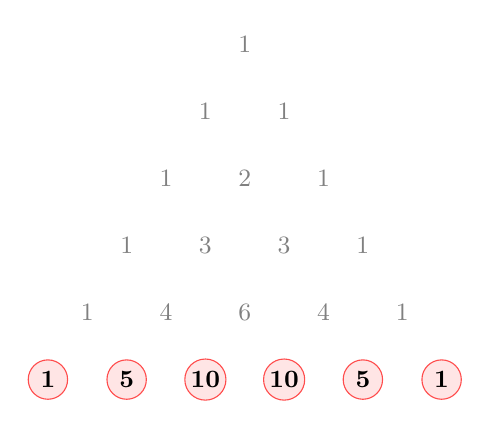
\begin{tikzpicture}[font=\small]
\node[gray] at (0,0) {$1$};
\node[gray] at (-0.5,-0.85) {$1$};
\node[gray] at (0.5,-0.85) {$1$};
\node[gray] at (-1,-1.7) {$1$};
\node[gray] at (0,-1.7) {$2$};
\node[gray] at (1,-1.7) {$1$};
\node[gray] at (-1.5,-2.55) {$1$};
\node[gray] at (-0.5,-2.55) {$3$};
\node[gray] at (0.5,-2.55) {$3$};
\node[gray] at (1.5,-2.55) {$1$};
\node[gray] at (-2,-3.4) {$1$};
\node[gray] at (-1,-3.4) {$4$};
\node[gray] at (0,-3.4) {$6$};
\node[gray] at (1,-3.4) {$4$};
\node[gray] at (2,-3.4) {$1$};
\node[circle,draw=red!70,fill=red!10,inner sep=1pt,minimum size=5mm] at (-2.5,-4.25) {$\mathbf{1}$};
\node[circle,draw=red!70,fill=red!10,inner sep=1pt,minimum size=5mm] at (-1.5,-4.25) {$\mathbf{5}$};
\node[circle,draw=red!70,fill=red!10,inner sep=1pt,minimum size=5mm] at (-0.5,-4.25) {$\mathbf{10}$};
\node[circle,draw=red!70,fill=red!10,inner sep=1pt,minimum size=5mm] at (0.5,-4.25) {$\mathbf{10}$};
\node[circle,draw=red!70,fill=red!10,inner sep=1pt,minimum size=5mm] at (1.5,-4.25) {$\mathbf{5}$};
\node[circle,draw=red!70,fill=red!10,inner sep=1pt,minimum size=5mm] at (2.5,-4.25) {$\mathbf{1}$};
\end{tikzpicture}
}
\end{center}
\small Row $5$ of Pascal's triangle (red) gives the binomial coefficients $\binom{5}{r}$; multiply each by the matching powers $a^{\,5-r}b^{\,r}$.\normalsize

\medskip\hrule

\section*{Binomial Expansion 33\quad\small\texttt{(be-033)}}
\addcontentsline{toc}{section}{Binomial Expansion 33 (be-033)}
\textit{Difficulty: Foundation \quad\textbar\quad Marks: 8}

\question{(a) Write down the first four terms, in ascending powers of \( x \), of the binomial expansion of \( (1 + x)^{12} \). \\[3pt] (b) Hence, or otherwise, find the first four terms of the expansion of \( (1 + x + x^2)(1 + x)^{12} \).}

\textbf{Worked solution.}

\textit{Step 1: Use the formula \(\binom{n}{r} = \frac{n!}{r!(n-r)!}\).}
\[\begin{gathered}
(1+x)^{12} \approx 1 + 12x + 66x^2 + 220x^3 + \ldots
\end{gathered}\]
(a) The first four terms are:

\textit{Step 2: Simplify each term.}
\[\begin{gathered}
1 \times (1 + 12x + 66x^2 + 220x^3) + x \times (1 + 12x + 66x^2) + x^2 \times (1 + 12x)
\end{gathered}\]
(b) Multiply \((1 + x + x^2)\) by \((1 + 12x + 66x^2 + 220x^3 + \ldots)\). Collect terms up to \(x^3\):

\textit{Step 3: Collect and simplify.}
\[\begin{gathered}
= (1) + (12 + 1)x + (66 + 12 + 1)x^2 + (220 + 66 + 12)x^3 + \ldots
\end{gathered}\]
Combine like terms:

\textit{Step 4: Final simplification.}
\[\begin{gathered}
= 1 + 13x + 79x^2 + 298x^3 + \ldots
\end{gathered}\]
Simplify:

\begin{answerbox}
\textbf{Final answer:}\quad \(\displaystyle (a) 1 + 12x + 66x^2 + 220x^3; (b) 1 + 13x + 79x^2 + 298x^3 + \ldots\)
\end{answerbox}
\textbf{Diagram.}

\begin{center}
\resizebox{\ifdim\width>\linewidth \linewidth\else \width\fi}{!}{%
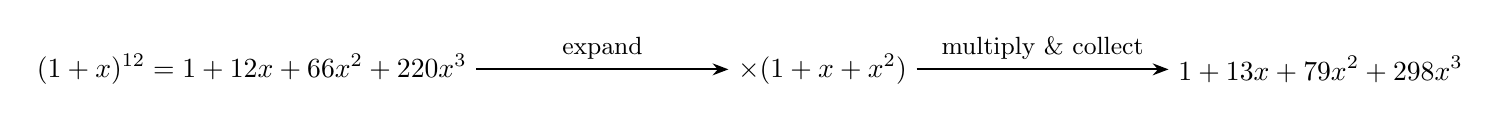
\begin{tikzpicture}[>={Stealth[length=2mm]},node distance=1.5cm and 3.2cm]
\node (s0) {$\displaystyle (1+x)^{12}=1+12x+66x^{2}+220x^{3}$};
\node (s1) [right=of s0] {$\displaystyle \times(1+x+x^{2})$};
\node (s2) [right=of s1] {$\displaystyle 1+13x+79x^{2}+298x^{3}$};
\draw[->,thick] (s0) -- (s1) node[midway,above,font=\small]{expand};
\draw[->,thick] (s1) -- (s2) node[midway,above,font=\small]{multiply \& collect};
\end{tikzpicture}
}
\end{center}
\small Solution flow: each arrow applies one step.\normalsize

\medskip\hrule

\section*{Binomial Expansion 34\quad\small\texttt{(be-034)}}
\addcontentsline{toc}{section}{Binomial Expansion 34 (be-034)}
\textit{Difficulty: Foundation \quad\textbar\quad Marks: 8}

\question{(a) Find the first four terms, in ascending powers of \( x \), of the expansion of \( (2 + x)^6 \). \\[3pt] (b) Use your expansion to show that \( (2 + x)^6 \approx 64 + 192x + 240x^2 + 160x^3 \) for small \( x \). \\[3pt] (c) By substituting \( x = 0.1 \), use the expansion to estimate \( 2.1^6 \) to 3 significant figures.}

\textbf{Worked solution.}

\textit{Step 1: Apply the binomial theorem: \((a+b)^n = \sum_{r=0}^{n} \binom{n}{r} a^{n-r} b^r\). Write the first few terms.}
\[\begin{gathered}
(2+x)^6 = 64 + 6 \times 32 x + 15 \times 16 x^2 + 20 \times 8 x^3 + \ldots
\end{gathered}\]
(a) General term: \(\binom{6}{r} 2^{6-r} x^r\). First four terms (\(r = 0, 1, 2, 3\)):

\textit{Step 2: Simplify.}
\[\begin{gathered}
= 64 + 192x + 240x^2 + 160x^3 + \ldots
\end{gathered}\]
Simplify:

\textit{Step 3: Collect and simplify.}
(b) This confirms the four-term approximation for small \(x\). $\checkmark$

\textit{Step 4: Final simplification.}
\[\begin{gathered}
2.1^6 \approx 64 + 192(0.1) + 240(0.01) + 160(0.001) = 64 + 19.2 + 2.4 + 0.16 = 85.76
\end{gathered}\]
(c) Substitute \(x = 0.1\):

\textit{Step 5: Final answer.}
\[\begin{gathered}
2.1^6 \approx 85.8
\end{gathered}\]
Round to 3 significant figures:

\begin{answerbox}
\textbf{Final answer:}\quad \(\displaystyle (a) 64 + 192x + 240x^2 + 160x^3; (c) 2.1^6 \approx 85.8\)
\end{answerbox}
\textbf{Diagram.}

\begin{center}
\resizebox{\ifdim\width>\linewidth \linewidth\else \width\fi}{!}{%
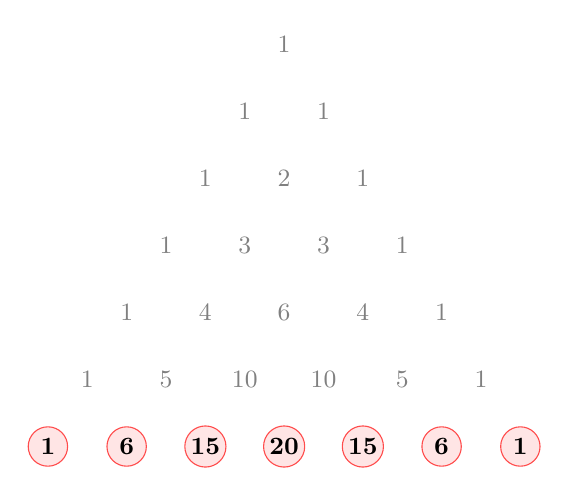
\begin{tikzpicture}[font=\small]
\node[gray] at (0,0) {$1$};
\node[gray] at (-0.5,-0.85) {$1$};
\node[gray] at (0.5,-0.85) {$1$};
\node[gray] at (-1,-1.7) {$1$};
\node[gray] at (0,-1.7) {$2$};
\node[gray] at (1,-1.7) {$1$};
\node[gray] at (-1.5,-2.55) {$1$};
\node[gray] at (-0.5,-2.55) {$3$};
\node[gray] at (0.5,-2.55) {$3$};
\node[gray] at (1.5,-2.55) {$1$};
\node[gray] at (-2,-3.4) {$1$};
\node[gray] at (-1,-3.4) {$4$};
\node[gray] at (0,-3.4) {$6$};
\node[gray] at (1,-3.4) {$4$};
\node[gray] at (2,-3.4) {$1$};
\node[gray] at (-2.5,-4.25) {$1$};
\node[gray] at (-1.5,-4.25) {$5$};
\node[gray] at (-0.5,-4.25) {$10$};
\node[gray] at (0.5,-4.25) {$10$};
\node[gray] at (1.5,-4.25) {$5$};
\node[gray] at (2.5,-4.25) {$1$};
\node[circle,draw=red!70,fill=red!10,inner sep=1pt,minimum size=5mm] at (-3,-5.1) {$\mathbf{1}$};
\node[circle,draw=red!70,fill=red!10,inner sep=1pt,minimum size=5mm] at (-2,-5.1) {$\mathbf{6}$};
\node[circle,draw=red!70,fill=red!10,inner sep=1pt,minimum size=5mm] at (-1,-5.1) {$\mathbf{15}$};
\node[circle,draw=red!70,fill=red!10,inner sep=1pt,minimum size=5mm] at (0,-5.1) {$\mathbf{20}$};
\node[circle,draw=red!70,fill=red!10,inner sep=1pt,minimum size=5mm] at (1,-5.1) {$\mathbf{15}$};
\node[circle,draw=red!70,fill=red!10,inner sep=1pt,minimum size=5mm] at (2,-5.1) {$\mathbf{6}$};
\node[circle,draw=red!70,fill=red!10,inner sep=1pt,minimum size=5mm] at (3,-5.1) {$\mathbf{1}$};
\end{tikzpicture}
}
\end{center}
\small Row $6$ of Pascal's triangle (red) gives the binomial coefficients $\binom{6}{r}$; multiply each by the matching powers $a^{\,6-r}b^{\,r}$.\normalsize

\medskip\hrule

\section*{Binomial Expansion 35\quad\small\texttt{(be-035)}}
\addcontentsline{toc}{section}{Binomial Expansion 35 (be-035)}
\textit{Difficulty: Foundation \quad\textbar\quad Marks: 9}

\question{(a) Write down the first four terms, in ascending powers of \( x \), of the expansion of \( (1 - x)^8 \). \\[3pt] (b) Hence find the first four terms of the expansion of \( (3 + x)(1 - x)^8 \). \\[3pt] (c) Find the coefficient of \( x^2 \) in the expansion of \( (3 + x)(1 - x)^8 \).}

\textbf{Worked solution.}

\textit{Step 1: Apply the binomial theorem: \((a+b)^n = \sum_{r=0}^{n} \binom{n}{r} a^{n-r} b^r\). Write the first few terms.}
\[\begin{gathered}
(1-x)^8 = 1 - 8x + 28x^2 - 56x^3 + \ldots
\end{gathered}\]
(a) Use \(b = -x\), \(n = 8\):

\textit{Step 2: Simplify each term.}
\[\begin{gathered}
3(1 - 8x + 28x^2 - 56x^3) + x(1 - 8x + 28x^2)
\end{gathered}\]
(b) Multiply \((3 + x)\) by \((1 - 8x + 28x^2 - 56x^3 + \ldots)\):

\textit{Step 3: Collect and simplify.}
\[\begin{gathered}
= 3 + (-24 + 1)x + (84 - 8)x^2 + (-168 + 28)x^3 + \ldots
\end{gathered}\]
Collect terms:

\textit{Step 4: Final simplification.}
\[\begin{gathered}
= 3 - 23x + 76x^2 - 140x^3 + \ldots
\end{gathered}\]
Simplify:

\textit{Step 5: Final answer.}
\[\begin{gathered}
\text{Coefficient of } x^2 = 76
\end{gathered}\]
(c) The coefficient of \(x^2\) is \(76\).

\begin{answerbox}
\textbf{Final answer:}\quad \(\displaystyle (a) 1 - 8x + 28x^2 - 56x^3; (b) 3 - 23x + 76x^2 - 140x^3 + \ldots; (c) 76\)
\end{answerbox}
\textbf{Diagram.}

\begin{center}
\resizebox{\ifdim\width>\linewidth \linewidth\else \width\fi}{!}{%
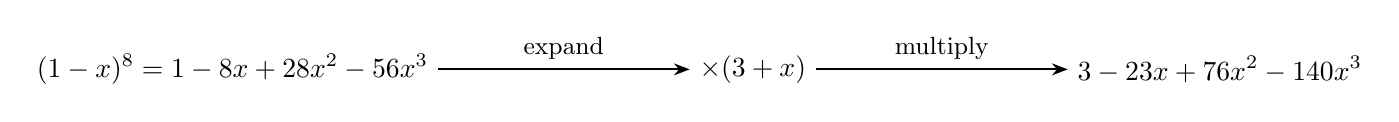
\begin{tikzpicture}[>={Stealth[length=2mm]},node distance=1.5cm and 3.2cm]
\node (s0) {$\displaystyle (1-x)^{8}=1-8x+28x^{2}-56x^{3}$};
\node (s1) [right=of s0] {$\displaystyle \times(3+x)$};
\node (s2) [right=of s1] {$\displaystyle 3-23x+76x^{2}-140x^{3}$};
\draw[->,thick] (s0) -- (s1) node[midway,above,font=\small]{expand};
\draw[->,thick] (s1) -- (s2) node[midway,above,font=\small]{multiply};
\end{tikzpicture}
}
\end{center}
\small Solution flow: each arrow applies one step.\normalsize

\medskip\hrule

\section*{Binomial Expansion 36\quad\small\texttt{(be-036)}}
\addcontentsline{toc}{section}{Binomial Expansion 36 (be-036)}
\textit{Difficulty: Foundation \quad\textbar\quad Marks: 3}

\question{Expand \( (1 + 2x)^4 \) in ascending powers of \( x \), up to and including the term in \( x^3 \).}

\textbf{Worked solution.}

\textit{Step 1: Apply the binomial theorem}
\[\begin{gathered}
\binom{4}{0} + \binom{4}{1}(2x) + \binom{4}{2}(2x)^2 + \binom{4}{3}(2x)^3
\end{gathered}\]
Use \( (1+2x)^4 \) with \( b = 2x \), \( n = 4 \).

\textit{Step 2: Simplify}
\[\begin{gathered}
1 + 8x + 24x^2 + 32x^3
\end{gathered}\]
Evaluate each term.

\begin{answerbox}
\textbf{Final answer:}\quad \(\displaystyle 1 + 8x + 24x^2 + 32x^3\)
\end{answerbox}
\textbf{Diagram.}

\begin{center}
\resizebox{\ifdim\width>\linewidth \linewidth\else \width\fi}{!}{%
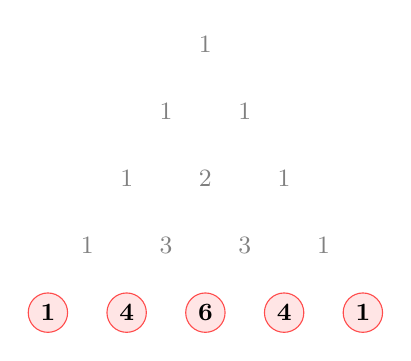
\begin{tikzpicture}[font=\small]
\node[gray] at (0,0) {$1$};
\node[gray] at (-0.5,-0.85) {$1$};
\node[gray] at (0.5,-0.85) {$1$};
\node[gray] at (-1,-1.7) {$1$};
\node[gray] at (0,-1.7) {$2$};
\node[gray] at (1,-1.7) {$1$};
\node[gray] at (-1.5,-2.55) {$1$};
\node[gray] at (-0.5,-2.55) {$3$};
\node[gray] at (0.5,-2.55) {$3$};
\node[gray] at (1.5,-2.55) {$1$};
\node[circle,draw=red!70,fill=red!10,inner sep=1pt,minimum size=5mm] at (-2,-3.4) {$\mathbf{1}$};
\node[circle,draw=red!70,fill=red!10,inner sep=1pt,minimum size=5mm] at (-1,-3.4) {$\mathbf{4}$};
\node[circle,draw=red!70,fill=red!10,inner sep=1pt,minimum size=5mm] at (0,-3.4) {$\mathbf{6}$};
\node[circle,draw=red!70,fill=red!10,inner sep=1pt,minimum size=5mm] at (1,-3.4) {$\mathbf{4}$};
\node[circle,draw=red!70,fill=red!10,inner sep=1pt,minimum size=5mm] at (2,-3.4) {$\mathbf{1}$};
\end{tikzpicture}
}
\end{center}
\small Row $4$ of Pascal's triangle (red) gives the binomial coefficients $\binom{4}{r}$; multiply each by the matching powers $a^{\,4-r}b^{\,r}$.\normalsize

\medskip\hrule

\section*{Binomial Expansion 37\quad\small\texttt{(be-037)}}
\addcontentsline{toc}{section}{Binomial Expansion 37 (be-037)}
\textit{Difficulty: Foundation \quad\textbar\quad Marks: 3}

\question{Expand \( (1 - 3x)^5 \) in ascending powers of \( x \), up to and including the term in \( x^3 \).}

\textbf{Worked solution.}

\textit{Step 1: Apply the binomial theorem}
\[\begin{gathered}
\binom{5}{0} + \binom{5}{1}(-3x) + \binom{5}{2}(-3x)^2 + \binom{5}{3}(-3x)^3
\end{gathered}\]
Use \( (1 + (-3x))^5 \).

\textit{Step 2: Simplify}
\[\begin{gathered}
1 - 15x + 90x^2 - 270x^3
\end{gathered}\]
Evaluate coefficients and signs.

\begin{answerbox}
\textbf{Final answer:}\quad \(\displaystyle 1 - 15x + 90x^2 - 270x^3\)
\end{answerbox}
\textbf{Diagram.}

\begin{center}
\resizebox{\ifdim\width>\linewidth \linewidth\else \width\fi}{!}{%
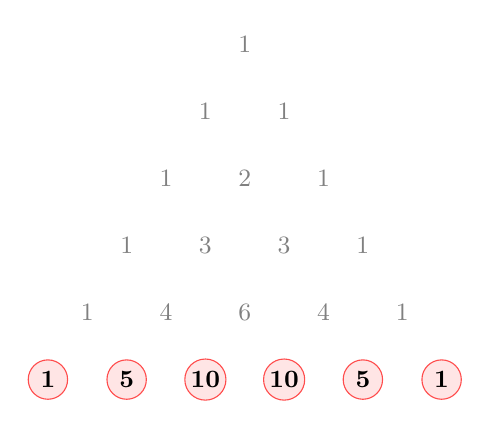
\begin{tikzpicture}[font=\small]
\node[gray] at (0,0) {$1$};
\node[gray] at (-0.5,-0.85) {$1$};
\node[gray] at (0.5,-0.85) {$1$};
\node[gray] at (-1,-1.7) {$1$};
\node[gray] at (0,-1.7) {$2$};
\node[gray] at (1,-1.7) {$1$};
\node[gray] at (-1.5,-2.55) {$1$};
\node[gray] at (-0.5,-2.55) {$3$};
\node[gray] at (0.5,-2.55) {$3$};
\node[gray] at (1.5,-2.55) {$1$};
\node[gray] at (-2,-3.4) {$1$};
\node[gray] at (-1,-3.4) {$4$};
\node[gray] at (0,-3.4) {$6$};
\node[gray] at (1,-3.4) {$4$};
\node[gray] at (2,-3.4) {$1$};
\node[circle,draw=red!70,fill=red!10,inner sep=1pt,minimum size=5mm] at (-2.5,-4.25) {$\mathbf{1}$};
\node[circle,draw=red!70,fill=red!10,inner sep=1pt,minimum size=5mm] at (-1.5,-4.25) {$\mathbf{5}$};
\node[circle,draw=red!70,fill=red!10,inner sep=1pt,minimum size=5mm] at (-0.5,-4.25) {$\mathbf{10}$};
\node[circle,draw=red!70,fill=red!10,inner sep=1pt,minimum size=5mm] at (0.5,-4.25) {$\mathbf{10}$};
\node[circle,draw=red!70,fill=red!10,inner sep=1pt,minimum size=5mm] at (1.5,-4.25) {$\mathbf{5}$};
\node[circle,draw=red!70,fill=red!10,inner sep=1pt,minimum size=5mm] at (2.5,-4.25) {$\mathbf{1}$};
\end{tikzpicture}
}
\end{center}
\small Row $5$ of Pascal's triangle (red) gives the binomial coefficients $\binom{5}{r}$; multiply each by the matching powers $a^{\,5-r}b^{\,r}$.\normalsize

\medskip\hrule

\section*{Binomial Expansion 38\quad\small\texttt{(be-038)}}
\addcontentsline{toc}{section}{Binomial Expansion 38 (be-038)}
\textit{Difficulty: Foundation \quad\textbar\quad Marks: 4}

\question{Find the first 4 terms in the expansion of \( (2 + x)^6 \) in ascending powers of \( x \).}

\textbf{Worked solution.}

\textit{Step 1: Apply the binomial theorem}
\[\begin{gathered}
\binom{6}{0}2^6 + \binom{6}{1}2^5 x + \binom{6}{2}2^4 x^2 + \binom{6}{3}2^3 x^3
\end{gathered}\]
With \( a=2, b=x, n=6 \).

\textit{Step 2: Simplify}
\[\begin{gathered}
64 + 192x + 240x^2 + 160x^3
\end{gathered}\]
Evaluate each term.

\begin{answerbox}
\textbf{Final answer:}\quad \(\displaystyle 64 + 192x + 240x^2 + 160x^3\)
\end{answerbox}
\textbf{Diagram.}

\begin{center}
\resizebox{\ifdim\width>\linewidth \linewidth\else \width\fi}{!}{%
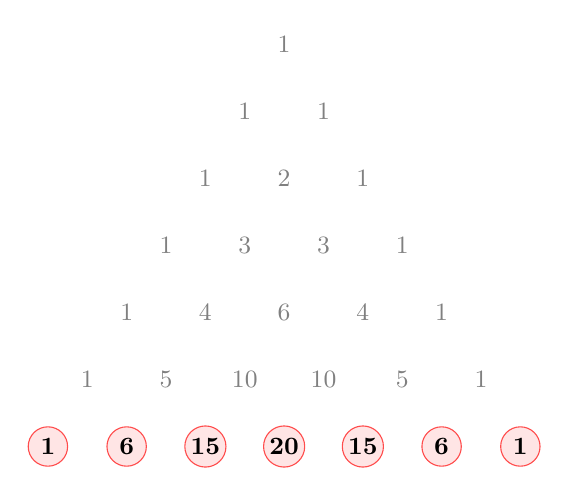
\begin{tikzpicture}[font=\small]
\node[gray] at (0,0) {$1$};
\node[gray] at (-0.5,-0.85) {$1$};
\node[gray] at (0.5,-0.85) {$1$};
\node[gray] at (-1,-1.7) {$1$};
\node[gray] at (0,-1.7) {$2$};
\node[gray] at (1,-1.7) {$1$};
\node[gray] at (-1.5,-2.55) {$1$};
\node[gray] at (-0.5,-2.55) {$3$};
\node[gray] at (0.5,-2.55) {$3$};
\node[gray] at (1.5,-2.55) {$1$};
\node[gray] at (-2,-3.4) {$1$};
\node[gray] at (-1,-3.4) {$4$};
\node[gray] at (0,-3.4) {$6$};
\node[gray] at (1,-3.4) {$4$};
\node[gray] at (2,-3.4) {$1$};
\node[gray] at (-2.5,-4.25) {$1$};
\node[gray] at (-1.5,-4.25) {$5$};
\node[gray] at (-0.5,-4.25) {$10$};
\node[gray] at (0.5,-4.25) {$10$};
\node[gray] at (1.5,-4.25) {$5$};
\node[gray] at (2.5,-4.25) {$1$};
\node[circle,draw=red!70,fill=red!10,inner sep=1pt,minimum size=5mm] at (-3,-5.1) {$\mathbf{1}$};
\node[circle,draw=red!70,fill=red!10,inner sep=1pt,minimum size=5mm] at (-2,-5.1) {$\mathbf{6}$};
\node[circle,draw=red!70,fill=red!10,inner sep=1pt,minimum size=5mm] at (-1,-5.1) {$\mathbf{15}$};
\node[circle,draw=red!70,fill=red!10,inner sep=1pt,minimum size=5mm] at (0,-5.1) {$\mathbf{20}$};
\node[circle,draw=red!70,fill=red!10,inner sep=1pt,minimum size=5mm] at (1,-5.1) {$\mathbf{15}$};
\node[circle,draw=red!70,fill=red!10,inner sep=1pt,minimum size=5mm] at (2,-5.1) {$\mathbf{6}$};
\node[circle,draw=red!70,fill=red!10,inner sep=1pt,minimum size=5mm] at (3,-5.1) {$\mathbf{1}$};
\end{tikzpicture}
}
\end{center}
\small Row $6$ of Pascal's triangle (red) gives the binomial coefficients $\binom{6}{r}$; multiply each by the matching powers $a^{\,6-r}b^{\,r}$.\normalsize

\medskip\hrule

\section*{Binomial Expansion 39\quad\small\texttt{(be-039)}}
\addcontentsline{toc}{section}{Binomial Expansion 39 (be-039)}
\textit{Difficulty: Foundation \quad\textbar\quad Marks: 3}

\question{Find the coefficient of \( x^3 \) in the expansion of \( (1 + 4x)^5 \).}

\textbf{Worked solution.}

\textit{Step 1: General term}
\[\begin{gathered}
\binom{5}{3} \times 4^3 \times x^3 = 10 \times 64 \times x^3
\end{gathered}\]
The term in \( x^3 \) is \( \binom{5}{3}(4x)^3 \).

\textit{Step 2: Evaluate}
\[\begin{gathered}
640x^3
\end{gathered}\]
Multiply.

\begin{answerbox}
\textbf{Final answer:}\quad \(\displaystyle 640\)
\end{answerbox}
\textbf{Diagram.}

\begin{center}
\resizebox{\ifdim\width>\linewidth \linewidth\else \width\fi}{!}{%
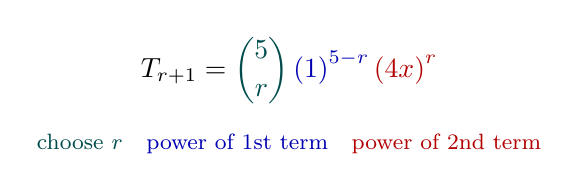
\begin{tikzpicture}
\node (T) {$\displaystyle T_{r+1} = {\color{teal!60!black}\binom{5}{r}}\,{\color{blue!70!black}\left(1\right)^{5-r}}\,{\color{red!70!black}\left(4x\right)^{r}}$};
\node[below=4pt of T,font=\footnotesize] {{\color{teal!60!black}choose $r$}\quad{\color{blue!70!black}power of 1st term}\quad{\color{red!70!black}power of 2nd term}};
\end{tikzpicture}
}
\end{center}
\small General term of $\left(1+4x\right)^{5}$. Set the power of $x$ to the required value to find $r$, then evaluate.\normalsize

\medskip\hrule

\section*{Binomial Expansion 40\quad\small\texttt{(be-040)}}
\addcontentsline{toc}{section}{Binomial Expansion 40 (be-040)}
\textit{Difficulty: Foundation \quad\textbar\quad Marks: 3}

\question{Find the coefficient of \( x^2 \) in the expansion of \( (3 - x)^6 \).}

\textbf{Worked solution.}

\textit{Step 1: General term for x\textasciicircum 2}
\[\begin{gathered}
\binom{6}{2} \times 81 \times x^2 = 15 \times 81 \times x^2
\end{gathered}\]
The \( x^2 \) term is \( \binom{6}{2}(3)^4(-x)^2 \).

\textit{Step 2: Evaluate}
\[\begin{gathered}
1215x^2
\end{gathered}\]
Multiply.

\begin{answerbox}
\textbf{Final answer:}\quad \(\displaystyle 1215\)
\end{answerbox}
\textbf{Diagram.}

\begin{center}
\resizebox{\ifdim\width>\linewidth \linewidth\else \width\fi}{!}{%
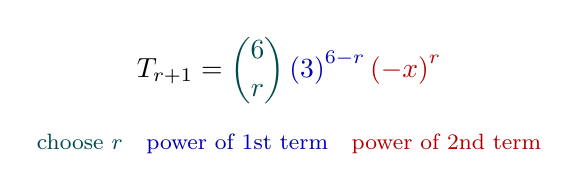
\begin{tikzpicture}
\node (T) {$\displaystyle T_{r+1} = {\color{teal!60!black}\binom{6}{r}}\,{\color{blue!70!black}\left(3\right)^{6-r}}\,{\color{red!70!black}\left(-x\right)^{r}}$};
\node[below=4pt of T,font=\footnotesize] {{\color{teal!60!black}choose $r$}\quad{\color{blue!70!black}power of 1st term}\quad{\color{red!70!black}power of 2nd term}};
\end{tikzpicture}
}
\end{center}
\small General term of $\left(3+-x\right)^{6}$. Set the power of $x$ to the required value to find $r$, then evaluate.\normalsize

\medskip\hrule

\section*{Binomial Expansion 41\quad\small\texttt{(be-041)}}
\addcontentsline{toc}{section}{Binomial Expansion 41 (be-041)}
\textit{Difficulty: Foundation \quad\textbar\quad Marks: 3}

\question{Expand \( (1 + x)^8 \) up to and including the term in \( x^3 \).}

\textbf{Worked solution.}

\textit{Step 1: First 4 terms}
\[\begin{gathered}
\binom{8}{0} + \binom{8}{1}x + \binom{8}{2}x^2 + \binom{8}{3}x^3
\end{gathered}\]
Apply the binomial theorem with \( n = 8 \).

\textit{Step 2: Evaluate}
\[\begin{gathered}
1 + 8x + 28x^2 + 56x^3
\end{gathered}\]
Compute coefficients.

\begin{answerbox}
\textbf{Final answer:}\quad \(\displaystyle 1 + 8x + 28x^2 + 56x^3\)
\end{answerbox}
\textbf{Diagram.}

\begin{center}
\resizebox{\ifdim\width>\linewidth \linewidth\else \width\fi}{!}{%
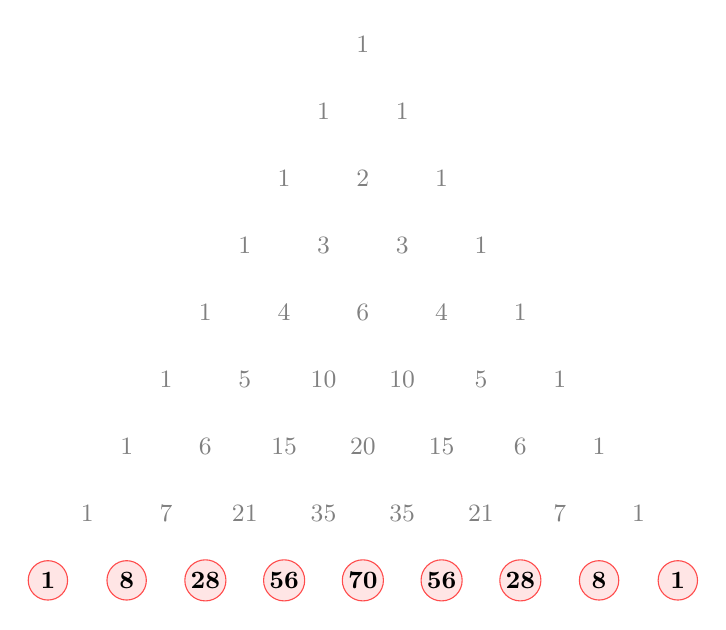
\begin{tikzpicture}[font=\small]
\node[gray] at (0,0) {$1$};
\node[gray] at (-0.5,-0.85) {$1$};
\node[gray] at (0.5,-0.85) {$1$};
\node[gray] at (-1,-1.7) {$1$};
\node[gray] at (0,-1.7) {$2$};
\node[gray] at (1,-1.7) {$1$};
\node[gray] at (-1.5,-2.55) {$1$};
\node[gray] at (-0.5,-2.55) {$3$};
\node[gray] at (0.5,-2.55) {$3$};
\node[gray] at (1.5,-2.55) {$1$};
\node[gray] at (-2,-3.4) {$1$};
\node[gray] at (-1,-3.4) {$4$};
\node[gray] at (0,-3.4) {$6$};
\node[gray] at (1,-3.4) {$4$};
\node[gray] at (2,-3.4) {$1$};
\node[gray] at (-2.5,-4.25) {$1$};
\node[gray] at (-1.5,-4.25) {$5$};
\node[gray] at (-0.5,-4.25) {$10$};
\node[gray] at (0.5,-4.25) {$10$};
\node[gray] at (1.5,-4.25) {$5$};
\node[gray] at (2.5,-4.25) {$1$};
\node[gray] at (-3,-5.1) {$1$};
\node[gray] at (-2,-5.1) {$6$};
\node[gray] at (-1,-5.1) {$15$};
\node[gray] at (0,-5.1) {$20$};
\node[gray] at (1,-5.1) {$15$};
\node[gray] at (2,-5.1) {$6$};
\node[gray] at (3,-5.1) {$1$};
\node[gray] at (-3.5,-5.95) {$1$};
\node[gray] at (-2.5,-5.95) {$7$};
\node[gray] at (-1.5,-5.95) {$21$};
\node[gray] at (-0.5,-5.95) {$35$};
\node[gray] at (0.5,-5.95) {$35$};
\node[gray] at (1.5,-5.95) {$21$};
\node[gray] at (2.5,-5.95) {$7$};
\node[gray] at (3.5,-5.95) {$1$};
\node[circle,draw=red!70,fill=red!10,inner sep=1pt,minimum size=5mm] at (-4,-6.8) {$\mathbf{1}$};
\node[circle,draw=red!70,fill=red!10,inner sep=1pt,minimum size=5mm] at (-3,-6.8) {$\mathbf{8}$};
\node[circle,draw=red!70,fill=red!10,inner sep=1pt,minimum size=5mm] at (-2,-6.8) {$\mathbf{28}$};
\node[circle,draw=red!70,fill=red!10,inner sep=1pt,minimum size=5mm] at (-1,-6.8) {$\mathbf{56}$};
\node[circle,draw=red!70,fill=red!10,inner sep=1pt,minimum size=5mm] at (0,-6.8) {$\mathbf{70}$};
\node[circle,draw=red!70,fill=red!10,inner sep=1pt,minimum size=5mm] at (1,-6.8) {$\mathbf{56}$};
\node[circle,draw=red!70,fill=red!10,inner sep=1pt,minimum size=5mm] at (2,-6.8) {$\mathbf{28}$};
\node[circle,draw=red!70,fill=red!10,inner sep=1pt,minimum size=5mm] at (3,-6.8) {$\mathbf{8}$};
\node[circle,draw=red!70,fill=red!10,inner sep=1pt,minimum size=5mm] at (4,-6.8) {$\mathbf{1}$};
\end{tikzpicture}
}
\end{center}
\small Row $8$ of Pascal's triangle (red) gives the binomial coefficients $\binom{8}{r}$; multiply each by the matching powers $a^{\,8-r}b^{\,r}$.\normalsize

\medskip\hrule

\section*{Binomial Expansion 42\quad\small\texttt{(be-042)}}
\addcontentsline{toc}{section}{Binomial Expansion 42 (be-042)}
\textit{Difficulty: Foundation \quad\textbar\quad Marks: 3}

\question{Expand \( (1 - 2x)^6 \) up to and including the term in \( x^3 \).}

\textbf{Worked solution.}

\textit{Step 1: Substitute b = -2x}
\[\begin{gathered}
\binom{6}{0} + \binom{6}{1}(-2x) + \binom{6}{2}(-2x)^2 + \binom{6}{3}(-2x)^3
\end{gathered}\]
Apply binomial theorem.

\textit{Step 2: Simplify}
\[\begin{gathered}
1 - 12x + 60x^2 - 160x^3
\end{gathered}\]
Evaluate each term.

\begin{answerbox}
\textbf{Final answer:}\quad \(\displaystyle 1 - 12x + 60x^2 - 160x^3\)
\end{answerbox}
\textbf{Diagram.}

\begin{center}
\resizebox{\ifdim\width>\linewidth \linewidth\else \width\fi}{!}{%
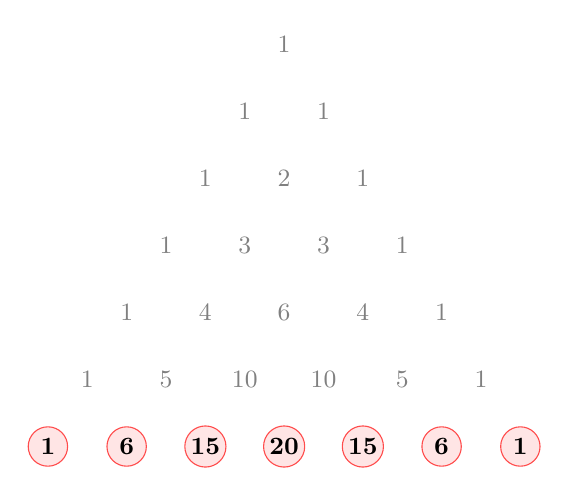
\begin{tikzpicture}[font=\small]
\node[gray] at (0,0) {$1$};
\node[gray] at (-0.5,-0.85) {$1$};
\node[gray] at (0.5,-0.85) {$1$};
\node[gray] at (-1,-1.7) {$1$};
\node[gray] at (0,-1.7) {$2$};
\node[gray] at (1,-1.7) {$1$};
\node[gray] at (-1.5,-2.55) {$1$};
\node[gray] at (-0.5,-2.55) {$3$};
\node[gray] at (0.5,-2.55) {$3$};
\node[gray] at (1.5,-2.55) {$1$};
\node[gray] at (-2,-3.4) {$1$};
\node[gray] at (-1,-3.4) {$4$};
\node[gray] at (0,-3.4) {$6$};
\node[gray] at (1,-3.4) {$4$};
\node[gray] at (2,-3.4) {$1$};
\node[gray] at (-2.5,-4.25) {$1$};
\node[gray] at (-1.5,-4.25) {$5$};
\node[gray] at (-0.5,-4.25) {$10$};
\node[gray] at (0.5,-4.25) {$10$};
\node[gray] at (1.5,-4.25) {$5$};
\node[gray] at (2.5,-4.25) {$1$};
\node[circle,draw=red!70,fill=red!10,inner sep=1pt,minimum size=5mm] at (-3,-5.1) {$\mathbf{1}$};
\node[circle,draw=red!70,fill=red!10,inner sep=1pt,minimum size=5mm] at (-2,-5.1) {$\mathbf{6}$};
\node[circle,draw=red!70,fill=red!10,inner sep=1pt,minimum size=5mm] at (-1,-5.1) {$\mathbf{15}$};
\node[circle,draw=red!70,fill=red!10,inner sep=1pt,minimum size=5mm] at (0,-5.1) {$\mathbf{20}$};
\node[circle,draw=red!70,fill=red!10,inner sep=1pt,minimum size=5mm] at (1,-5.1) {$\mathbf{15}$};
\node[circle,draw=red!70,fill=red!10,inner sep=1pt,minimum size=5mm] at (2,-5.1) {$\mathbf{6}$};
\node[circle,draw=red!70,fill=red!10,inner sep=1pt,minimum size=5mm] at (3,-5.1) {$\mathbf{1}$};
\end{tikzpicture}
}
\end{center}
\small Row $6$ of Pascal's triangle (red) gives the binomial coefficients $\binom{6}{r}$; multiply each by the matching powers $a^{\,6-r}b^{\,r}$.\normalsize

\medskip\hrule

\section*{Binomial Expansion 43\quad\small\texttt{(be-043)}}
\addcontentsline{toc}{section}{Binomial Expansion 43 (be-043)}
\textit{Difficulty: Foundation \quad\textbar\quad Marks: 4}

\question{Find the first 4 terms of \( (3 + 2x)^5 \) in ascending powers of \( x \).}

\textbf{Worked solution.}

\textit{Step 1: Apply binomial theorem}
\[\begin{gathered}
\binom{5}{0}3^5 + \binom{5}{1}3^4(2x) + \binom{5}{2}3^3(2x)^2 + \binom{5}{3}3^2(2x)^3
\end{gathered}\]
With \( a=3, b=2x, n=5 \).

\textit{Step 2: Evaluate}
\[\begin{gathered}
243 + 810x + 1080x^2 + 720x^3
\end{gathered}\]
Compute each term.

\begin{answerbox}
\textbf{Final answer:}\quad \(\displaystyle 243 + 810x + 1080x^2 + 720x^3\)
\end{answerbox}
\textbf{Diagram.}

\begin{center}
\resizebox{\ifdim\width>\linewidth \linewidth\else \width\fi}{!}{%
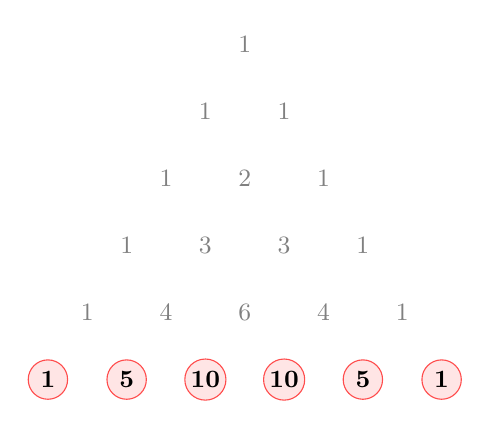
\begin{tikzpicture}[font=\small]
\node[gray] at (0,0) {$1$};
\node[gray] at (-0.5,-0.85) {$1$};
\node[gray] at (0.5,-0.85) {$1$};
\node[gray] at (-1,-1.7) {$1$};
\node[gray] at (0,-1.7) {$2$};
\node[gray] at (1,-1.7) {$1$};
\node[gray] at (-1.5,-2.55) {$1$};
\node[gray] at (-0.5,-2.55) {$3$};
\node[gray] at (0.5,-2.55) {$3$};
\node[gray] at (1.5,-2.55) {$1$};
\node[gray] at (-2,-3.4) {$1$};
\node[gray] at (-1,-3.4) {$4$};
\node[gray] at (0,-3.4) {$6$};
\node[gray] at (1,-3.4) {$4$};
\node[gray] at (2,-3.4) {$1$};
\node[circle,draw=red!70,fill=red!10,inner sep=1pt,minimum size=5mm] at (-2.5,-4.25) {$\mathbf{1}$};
\node[circle,draw=red!70,fill=red!10,inner sep=1pt,minimum size=5mm] at (-1.5,-4.25) {$\mathbf{5}$};
\node[circle,draw=red!70,fill=red!10,inner sep=1pt,minimum size=5mm] at (-0.5,-4.25) {$\mathbf{10}$};
\node[circle,draw=red!70,fill=red!10,inner sep=1pt,minimum size=5mm] at (0.5,-4.25) {$\mathbf{10}$};
\node[circle,draw=red!70,fill=red!10,inner sep=1pt,minimum size=5mm] at (1.5,-4.25) {$\mathbf{5}$};
\node[circle,draw=red!70,fill=red!10,inner sep=1pt,minimum size=5mm] at (2.5,-4.25) {$\mathbf{1}$};
\end{tikzpicture}
}
\end{center}
\small Row $5$ of Pascal's triangle (red) gives the binomial coefficients $\binom{5}{r}$; multiply each by the matching powers $a^{\,5-r}b^{\,r}$.\normalsize

\medskip\hrule

\section*{Binomial Expansion 44\quad\small\texttt{(be-044)}}
\addcontentsline{toc}{section}{Binomial Expansion 44 (be-044)}
\textit{Difficulty: Foundation \quad\textbar\quad Marks: 2}

\question{Find the coefficient of \( x^4 \) in the expansion of \( (1 + x)^{10} \).}

\textbf{Worked solution.}

\textit{Use the general term}
\[\begin{gathered}
\binom{10}{4} = \frac{10!}{4! \times 6!} = 210
\end{gathered}\]
Coefficient of \( x^4 \) is \( \binom{10}{4} \).

\begin{answerbox}
\textbf{Final answer:}\quad \(\displaystyle 210\)
\end{answerbox}
\textbf{Diagram.}

\begin{center}
\resizebox{\ifdim\width>\linewidth \linewidth\else \width\fi}{!}{%
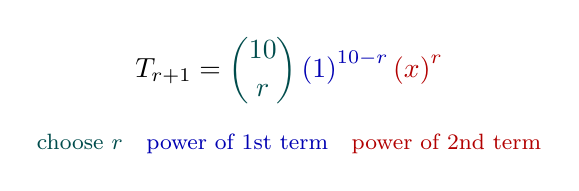
\begin{tikzpicture}
\node (T) {$\displaystyle T_{r+1} = {\color{teal!60!black}\binom{10}{r}}\,{\color{blue!70!black}\left(1\right)^{10-r}}\,{\color{red!70!black}\left(x\right)^{r}}$};
\node[below=4pt of T,font=\footnotesize] {{\color{teal!60!black}choose $r$}\quad{\color{blue!70!black}power of 1st term}\quad{\color{red!70!black}power of 2nd term}};
\end{tikzpicture}
}
\end{center}
\small General term of $\left(1+x\right)^{10}$. Set the power of $x$ to the required value to find $r$, then evaluate.\normalsize

\medskip\hrule

\section*{Binomial Expansion 45\quad\small\texttt{(be-045)}}
\addcontentsline{toc}{section}{Binomial Expansion 45 (be-045)}
\textit{Difficulty: Foundation \quad\textbar\quad Marks: 3}

\question{Find the coefficient of \( x^2 \) in the expansion of \( (1 - 5x)^4 \).}

\textbf{Worked solution.}

\textit{x\textasciicircum 2 term}
\[\begin{gathered}
\binom{4}{2} \times 25x^2 = 6 \times 25 = 150x^2
\end{gathered}\]
The term is \( \binom{4}{2}(-5x)^2 \).

\begin{answerbox}
\textbf{Final answer:}\quad \(\displaystyle 150\)
\end{answerbox}
\textbf{Diagram.}

\begin{center}
\resizebox{\ifdim\width>\linewidth \linewidth\else \width\fi}{!}{%
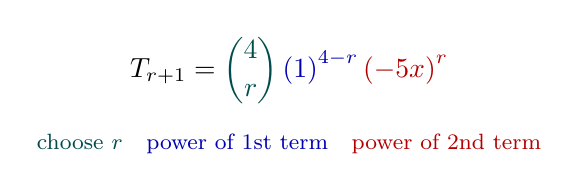
\begin{tikzpicture}
\node (T) {$\displaystyle T_{r+1} = {\color{teal!60!black}\binom{4}{r}}\,{\color{blue!70!black}\left(1\right)^{4-r}}\,{\color{red!70!black}\left(-5x\right)^{r}}$};
\node[below=4pt of T,font=\footnotesize] {{\color{teal!60!black}choose $r$}\quad{\color{blue!70!black}power of 1st term}\quad{\color{red!70!black}power of 2nd term}};
\end{tikzpicture}
}
\end{center}
\small General term of $\left(1+-5x\right)^{4}$. Set the power of $x$ to the required value to find $r$, then evaluate.\normalsize

\medskip\hrule

\section*{Binomial Expansion 46\quad\small\texttt{(be-046)}}
\addcontentsline{toc}{section}{Binomial Expansion 46 (be-046)}
\textit{Difficulty: Foundation \quad\textbar\quad Marks: 4}

\question{Expand \( (x - 2)^5 \) fully.}

\textbf{Worked solution.}

\textit{Step 1: Apply binomial theorem}
\[\begin{gathered}
\sum_{r=0}^{5} \binom{5}{r} x^{5-r}(-2)^r
\end{gathered}\]
With \( a=x, b=-2, n=5 \).

\textit{Step 2: Expand all terms}
\[\begin{gathered}
x^5 - 10x^4 + 40x^3 - 80x^2 + 80x - 32
\end{gathered}\]
Evaluate each term.

\begin{answerbox}
\textbf{Final answer:}\quad \(\displaystyle x^5 - 10x^4 + 40x^3 - 80x^2 + 80x - 32\)
\end{answerbox}
\textbf{Diagram.}

\begin{center}
\resizebox{\ifdim\width>\linewidth \linewidth\else \width\fi}{!}{%
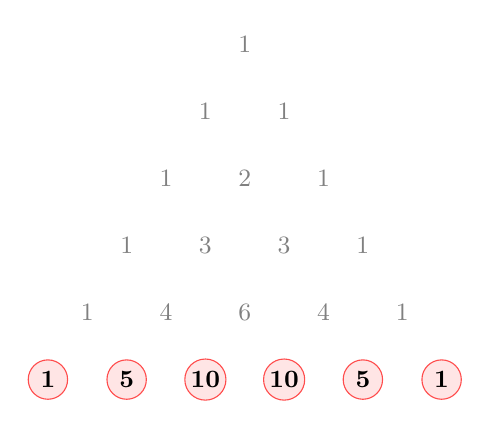
\begin{tikzpicture}[font=\small]
\node[gray] at (0,0) {$1$};
\node[gray] at (-0.5,-0.85) {$1$};
\node[gray] at (0.5,-0.85) {$1$};
\node[gray] at (-1,-1.7) {$1$};
\node[gray] at (0,-1.7) {$2$};
\node[gray] at (1,-1.7) {$1$};
\node[gray] at (-1.5,-2.55) {$1$};
\node[gray] at (-0.5,-2.55) {$3$};
\node[gray] at (0.5,-2.55) {$3$};
\node[gray] at (1.5,-2.55) {$1$};
\node[gray] at (-2,-3.4) {$1$};
\node[gray] at (-1,-3.4) {$4$};
\node[gray] at (0,-3.4) {$6$};
\node[gray] at (1,-3.4) {$4$};
\node[gray] at (2,-3.4) {$1$};
\node[circle,draw=red!70,fill=red!10,inner sep=1pt,minimum size=5mm] at (-2.5,-4.25) {$\mathbf{1}$};
\node[circle,draw=red!70,fill=red!10,inner sep=1pt,minimum size=5mm] at (-1.5,-4.25) {$\mathbf{5}$};
\node[circle,draw=red!70,fill=red!10,inner sep=1pt,minimum size=5mm] at (-0.5,-4.25) {$\mathbf{10}$};
\node[circle,draw=red!70,fill=red!10,inner sep=1pt,minimum size=5mm] at (0.5,-4.25) {$\mathbf{10}$};
\node[circle,draw=red!70,fill=red!10,inner sep=1pt,minimum size=5mm] at (1.5,-4.25) {$\mathbf{5}$};
\node[circle,draw=red!70,fill=red!10,inner sep=1pt,minimum size=5mm] at (2.5,-4.25) {$\mathbf{1}$};
\end{tikzpicture}
}
\end{center}
\small Row $5$ of Pascal's triangle (red) gives the binomial coefficients $\binom{5}{r}$; multiply each by the matching powers $a^{\,5-r}b^{\,r}$.\normalsize

\medskip\hrule

\section*{Binomial Expansion 47\quad\small\texttt{(be-047)}}
\addcontentsline{toc}{section}{Binomial Expansion 47 (be-047)}
\textit{Difficulty: Foundation \quad\textbar\quad Marks: 4}

\question{Find the term independent of \( x \) in the expansion of \( \left(x + \frac{2}{x}\right)^6 \).}

\textbf{Worked solution.}

\textit{Step 1: General term}
\[\begin{gathered}
x^{6-2r} = x^0 \implies r = 3
\end{gathered}\]
The general term is \( \binom{6}{r} x^{6-r} \left(\frac{2}{x}\right)^r = \binom{6}{r} 2^r x^{6-2r} \).

\textit{Step 2: Evaluate}
\[\begin{gathered}
\binom{6}{3} \times 2^3 = 20 \times 8 = 160
\end{gathered}\]
Substitute \( r = 3 \).

\begin{answerbox}
\textbf{Final answer:}\quad \(\displaystyle 160\)
\end{answerbox}
\textbf{Diagram.}

\begin{center}
\resizebox{\ifdim\width>\linewidth \linewidth\else \width\fi}{!}{%
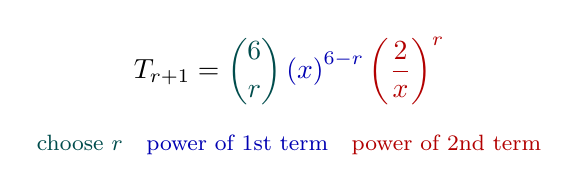
\begin{tikzpicture}
\node (T) {$\displaystyle T_{r+1} = {\color{teal!60!black}\binom{6}{r}}\,{\color{blue!70!black}\left(x\right)^{6-r}}\,{\color{red!70!black}\left(\frac{2}{x}\right)^{r}}$};
\node[below=4pt of T,font=\footnotesize] {{\color{teal!60!black}choose $r$}\quad{\color{blue!70!black}power of 1st term}\quad{\color{red!70!black}power of 2nd term}};
\end{tikzpicture}
}
\end{center}
\small General term of $\left(x+\frac{2}{x}\right)^{6}$. Set the power of $x$ to the required value to find $r$, then evaluate.\normalsize

\medskip\hrule

\section*{Binomial Expansion 48\quad\small\texttt{(be-048)}}
\addcontentsline{toc}{section}{Binomial Expansion 48 (be-048)}
\textit{Difficulty: Foundation \quad\textbar\quad Marks: 3}

\question{In the expansion of \( (1 + kx)^6 \), the coefficient of \( x^2 \) is 60. Find the value of \( k \), where \( k > 0 \).}

\textbf{Worked solution.}

\textit{Step 1: x\textasciicircum 2 coefficient}
\[\begin{gathered}
15k^2 = 60
\end{gathered}\]
The coefficient is \( \binom{6}{2} k^2 = 15k^2 \).

\textit{Step 2: Solve}
\[\begin{gathered}
k^2 = 4 \implies k = 2
\end{gathered}\]
Divide by 15 and take the positive root.

\begin{answerbox}
\textbf{Final answer:}\quad \(\displaystyle k = 2\)
\end{answerbox}
\textbf{Diagram.}

\begin{center}
\resizebox{\ifdim\width>\linewidth \linewidth\else \width\fi}{!}{%
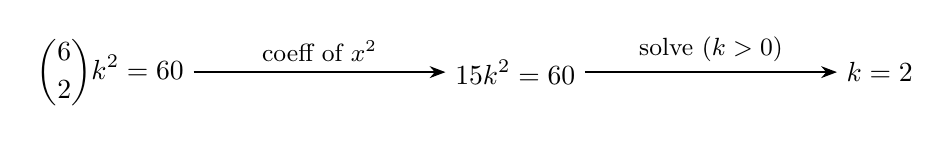
\begin{tikzpicture}[>={Stealth[length=2mm]},node distance=1.5cm and 3.2cm]
\node (s0) {$\displaystyle \binom{6}{2}k^{2}=60$};
\node (s1) [right=of s0] {$\displaystyle 15k^{2}=60$};
\node (s2) [right=of s1] {$\displaystyle k=2$};
\draw[->,thick] (s0) -- (s1) node[midway,above,font=\small]{coeff of $x^{2}$};
\draw[->,thick] (s1) -- (s2) node[midway,above,font=\small]{solve ($k>0$)};
\end{tikzpicture}
}
\end{center}
\small Solution flow: each arrow applies one step.\normalsize

\medskip\hrule

\section*{Binomial Expansion 49\quad\small\texttt{(be-049)}}
\addcontentsline{toc}{section}{Binomial Expansion 49 (be-049)}
\textit{Difficulty: Foundation \quad\textbar\quad Marks: 3}

\question{Find the first 3 terms of \( (1 + 3x)^{10} \) in ascending powers of \( x \).}

\textbf{Worked solution.}

\textit{Step 1: Apply binomial theorem}
\[\begin{gathered}
1 + \binom{10}{1}(3x) + \binom{10}{2}(3x)^2
\end{gathered}\]
First 3 terms with \( n=10, b=3x \).

\textit{Step 2: Evaluate}
\[\begin{gathered}
1 + 30x + 405x^2
\end{gathered}\]
Compute coefficients.

\begin{answerbox}
\textbf{Final answer:}\quad \(\displaystyle 1 + 30x + 405x^2\)
\end{answerbox}
\textbf{Diagram.}

\begin{center}
\resizebox{\ifdim\width>\linewidth \linewidth\else \width\fi}{!}{%
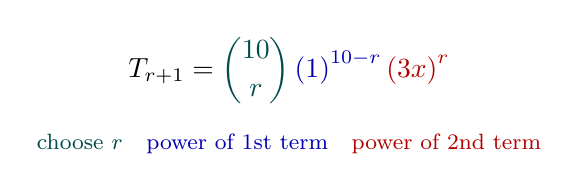
\begin{tikzpicture}
\node (T) {$\displaystyle T_{r+1} = {\color{teal!60!black}\binom{10}{r}}\,{\color{blue!70!black}\left(1\right)^{10-r}}\,{\color{red!70!black}\left(3x\right)^{r}}$};
\node[below=4pt of T,font=\footnotesize] {{\color{teal!60!black}choose $r$}\quad{\color{blue!70!black}power of 1st term}\quad{\color{red!70!black}power of 2nd term}};
\end{tikzpicture}
}
\end{center}
\small General term of $\left(1+3x\right)^{10}$. Set the power of $x$ to the required value to find $r$, then evaluate.\normalsize

\medskip\hrule

\section*{Binomial Expansion 50\quad\small\texttt{(be-050)}}
\addcontentsline{toc}{section}{Binomial Expansion 50 (be-050)}
\textit{Difficulty: Foundation \quad\textbar\quad Marks: 4}

\question{Expand \( (2x - 1)^4 \) fully.}

\textbf{Worked solution.}

\textit{Step 1: Apply binomial theorem}
\[\begin{gathered}
(2x)^4 + \binom{4}{1}(2x)^3(-1) + \binom{4}{2}(2x)^2(-1)^2 + \binom{4}{3}(2x)(-1)^3 + (-1)^4
\end{gathered}\]
With \( a=2x, b=-1, n=4 \).

\textit{Step 2: Simplify}
\[\begin{gathered}
16x^4 - 32x^3 + 24x^2 - 8x + 1
\end{gathered}\]
Evaluate.

\begin{answerbox}
\textbf{Final answer:}\quad \(\displaystyle 16x^4 - 32x^3 + 24x^2 - 8x + 1\)
\end{answerbox}
\textbf{Diagram.}

\begin{center}
\resizebox{\ifdim\width>\linewidth \linewidth\else \width\fi}{!}{%
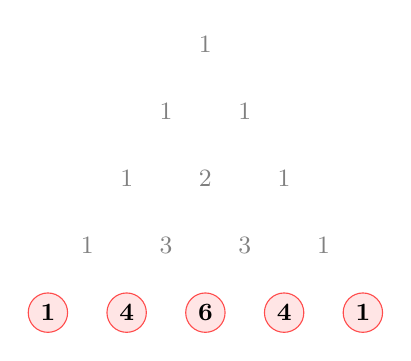
\begin{tikzpicture}[font=\small]
\node[gray] at (0,0) {$1$};
\node[gray] at (-0.5,-0.85) {$1$};
\node[gray] at (0.5,-0.85) {$1$};
\node[gray] at (-1,-1.7) {$1$};
\node[gray] at (0,-1.7) {$2$};
\node[gray] at (1,-1.7) {$1$};
\node[gray] at (-1.5,-2.55) {$1$};
\node[gray] at (-0.5,-2.55) {$3$};
\node[gray] at (0.5,-2.55) {$3$};
\node[gray] at (1.5,-2.55) {$1$};
\node[circle,draw=red!70,fill=red!10,inner sep=1pt,minimum size=5mm] at (-2,-3.4) {$\mathbf{1}$};
\node[circle,draw=red!70,fill=red!10,inner sep=1pt,minimum size=5mm] at (-1,-3.4) {$\mathbf{4}$};
\node[circle,draw=red!70,fill=red!10,inner sep=1pt,minimum size=5mm] at (0,-3.4) {$\mathbf{6}$};
\node[circle,draw=red!70,fill=red!10,inner sep=1pt,minimum size=5mm] at (1,-3.4) {$\mathbf{4}$};
\node[circle,draw=red!70,fill=red!10,inner sep=1pt,minimum size=5mm] at (2,-3.4) {$\mathbf{1}$};
\end{tikzpicture}
}
\end{center}
\small Row $4$ of Pascal's triangle (red) gives the binomial coefficients $\binom{4}{r}$; multiply each by the matching powers $a^{\,4-r}b^{\,r}$.\normalsize

\medskip\hrule

\section*{Binomial Expansion 51\quad\small\texttt{(be-051)}}
\addcontentsline{toc}{section}{Binomial Expansion 51 (be-051)}
\textit{Difficulty: Foundation \quad\textbar\quad Marks: 3}

\question{Find the coefficient of \( x^3 \) in the expansion of \( (2 - x)^7 \).}

\textbf{Worked solution.}

\textit{x\textasciicircum 3 term}
\[\begin{gathered}
\binom{7}{3} \times 16 \times (-x^3) = 35 \times 16 \times (-1) = -560
\end{gathered}\]
The term is \( \binom{7}{3}(2)^4(-x)^3 \).

\begin{answerbox}
\textbf{Final answer:}\quad \(\displaystyle -560\)
\end{answerbox}
\textbf{Diagram.}

\begin{center}
\resizebox{\ifdim\width>\linewidth \linewidth\else \width\fi}{!}{%
\begin{tikzpicture}
\node (T) {$\displaystyle T_{r+1} = {\color{teal!60!black}\binom{7}{r}}\,{\color{blue!70!black}\left(2\right)^{7-r}}\,{\color{red!70!black}\left(-x\right)^{r}}$};
\node[below=4pt of T,font=\footnotesize] {{\color{teal!60!black}choose $r$}\quad{\color{blue!70!black}power of 1st term}\quad{\color{red!70!black}power of 2nd term}};
\end{tikzpicture}
}
\end{center}
\small General term of $\left(2+-x\right)^{7}$. Set the power of $x$ to the required value to find $r$, then evaluate.\normalsize

\medskip\hrule

\section*{Binomial Expansion 52\quad\small\texttt{(be-052)}}
\addcontentsline{toc}{section}{Binomial Expansion 52 (be-052)}
\textit{Difficulty: Foundation \quad\textbar\quad Marks: 3}

\question{Expand \( (1 + x)^7 \) up to the term in \( x^4 \).}

\textbf{Worked solution.}

\textit{First 5 terms}
\[\begin{gathered}
1 + 7x + 21x^2 + 35x^3 + 35x^4
\end{gathered}\]
Apply binomial theorem.

\begin{answerbox}
\textbf{Final answer:}\quad \(\displaystyle 1 + 7x + 21x^2 + 35x^3 + 35x^4\)
\end{answerbox}
\textbf{Diagram.}

\begin{center}
\resizebox{\ifdim\width>\linewidth \linewidth\else \width\fi}{!}{%
\begin{tikzpicture}[font=\small]
\node[gray] at (0,0) {$1$};
\node[gray] at (-0.5,-0.85) {$1$};
\node[gray] at (0.5,-0.85) {$1$};
\node[gray] at (-1,-1.7) {$1$};
\node[gray] at (0,-1.7) {$2$};
\node[gray] at (1,-1.7) {$1$};
\node[gray] at (-1.5,-2.55) {$1$};
\node[gray] at (-0.5,-2.55) {$3$};
\node[gray] at (0.5,-2.55) {$3$};
\node[gray] at (1.5,-2.55) {$1$};
\node[gray] at (-2,-3.4) {$1$};
\node[gray] at (-1,-3.4) {$4$};
\node[gray] at (0,-3.4) {$6$};
\node[gray] at (1,-3.4) {$4$};
\node[gray] at (2,-3.4) {$1$};
\node[gray] at (-2.5,-4.25) {$1$};
\node[gray] at (-1.5,-4.25) {$5$};
\node[gray] at (-0.5,-4.25) {$10$};
\node[gray] at (0.5,-4.25) {$10$};
\node[gray] at (1.5,-4.25) {$5$};
\node[gray] at (2.5,-4.25) {$1$};
\node[gray] at (-3,-5.1) {$1$};
\node[gray] at (-2,-5.1) {$6$};
\node[gray] at (-1,-5.1) {$15$};
\node[gray] at (0,-5.1) {$20$};
\node[gray] at (1,-5.1) {$15$};
\node[gray] at (2,-5.1) {$6$};
\node[gray] at (3,-5.1) {$1$};
\node[circle,draw=red!70,fill=red!10,inner sep=1pt,minimum size=5mm] at (-3.5,-5.95) {$\mathbf{1}$};
\node[circle,draw=red!70,fill=red!10,inner sep=1pt,minimum size=5mm] at (-2.5,-5.95) {$\mathbf{7}$};
\node[circle,draw=red!70,fill=red!10,inner sep=1pt,minimum size=5mm] at (-1.5,-5.95) {$\mathbf{21}$};
\node[circle,draw=red!70,fill=red!10,inner sep=1pt,minimum size=5mm] at (-0.5,-5.95) {$\mathbf{35}$};
\node[circle,draw=red!70,fill=red!10,inner sep=1pt,minimum size=5mm] at (0.5,-5.95) {$\mathbf{35}$};
\node[circle,draw=red!70,fill=red!10,inner sep=1pt,minimum size=5mm] at (1.5,-5.95) {$\mathbf{21}$};
\node[circle,draw=red!70,fill=red!10,inner sep=1pt,minimum size=5mm] at (2.5,-5.95) {$\mathbf{7}$};
\node[circle,draw=red!70,fill=red!10,inner sep=1pt,minimum size=5mm] at (3.5,-5.95) {$\mathbf{1}$};
\end{tikzpicture}
}
\end{center}
\small Row $7$ of Pascal's triangle (red) gives the binomial coefficients $\binom{7}{r}$; multiply each by the matching powers $a^{\,7-r}b^{\,r}$.\normalsize

\medskip\hrule

\section*{Binomial Expansion 53\quad\small\texttt{(be-053)}}
\addcontentsline{toc}{section}{Binomial Expansion 53 (be-053)}
\textit{Difficulty: Foundation \quad\textbar\quad Marks: 3}

\question{Find the first 4 terms of \( (1 - x)^{12} \) in ascending powers of \( x \).}

\textbf{Worked solution.}

\textit{Apply binomial theorem}
\[\begin{gathered}
1 - 12x + 66x^2 - 220x^3
\end{gathered}\]
With \( b = -x, n = 12 \).

\begin{answerbox}
\textbf{Final answer:}\quad \(\displaystyle 1 - 12x + 66x^2 - 220x^3\)
\end{answerbox}
\textbf{Diagram.}

\begin{center}
\resizebox{\ifdim\width>\linewidth \linewidth\else \width\fi}{!}{%
\begin{tikzpicture}
\node (T) {$\displaystyle T_{r+1} = {\color{teal!60!black}\binom{12}{r}}\,{\color{blue!70!black}\left(1\right)^{12-r}}\,{\color{red!70!black}\left(-x\right)^{r}}$};
\node[below=4pt of T,font=\footnotesize] {{\color{teal!60!black}choose $r$}\quad{\color{blue!70!black}power of 1st term}\quad{\color{red!70!black}power of 2nd term}};
\end{tikzpicture}
}
\end{center}
\small General term of $\left(1+-x\right)^{12}$. Set the power of $x$ to the required value to find $r$, then evaluate.\normalsize

\medskip\hrule

\section*{Binomial Expansion 54\quad\small\texttt{(be-054)}}
\addcontentsline{toc}{section}{Binomial Expansion 54 (be-054)}
\textit{Difficulty: Foundation \quad\textbar\quad Marks: 3}

\question{In the expansion of \( (1 + ax)^8 \), the coefficient of \( x^3 \) is 1512. Find the value of \( a \).}

\textbf{Worked solution.}

\textit{Step 1: x\textasciicircum 3 coefficient}
\[\begin{gathered}
56a^3 = 1512
\end{gathered}\]
The coefficient is \( \binom{8}{3}a^3 = 56a^3 \).

\textit{Step 2: Solve}
\[\begin{gathered}
a^3 = 27 \implies a = 3
\end{gathered}\]
Divide and take cube root.

\begin{answerbox}
\textbf{Final answer:}\quad \(\displaystyle a = 3\)
\end{answerbox}
\textbf{Diagram.}

\begin{center}
\resizebox{\ifdim\width>\linewidth \linewidth\else \width\fi}{!}{%
\begin{tikzpicture}[>={Stealth[length=2mm]},node distance=1.5cm and 3.2cm]
\node (s0) {$\displaystyle \binom{8}{3}a^{3}=1512$};
\node (s1) [right=of s0] {$\displaystyle 56a^{3}=1512\Rightarrow a^{3}=27$};
\node (s2) [right=of s1] {$\displaystyle a=3$};
\draw[->,thick] (s0) -- (s1) node[midway,above,font=\small]{coeff of $x^{3}$};
\draw[->,thick] (s1) -- (s2) node[midway,above,font=\small]{solve};
\end{tikzpicture}
}
\end{center}
\small Solution flow: each arrow applies one step.\normalsize

\medskip\hrule

\section*{Binomial Expansion 55\quad\small\texttt{(be-055)}}
\addcontentsline{toc}{section}{Binomial Expansion 55 (be-055)}
\textit{Difficulty: Foundation \quad\textbar\quad Marks: 2}

\question{Find the coefficient of \( x^5 \) in \( (1 + x)^9 \).}

\textbf{Worked solution.}

\textit{Evaluate}
\[\begin{gathered}
\binom{9}{5} = \frac{9!}{5! \times 4!} = 126
\end{gathered}\]
The coefficient is \( \binom{9}{5} \).

\begin{answerbox}
\textbf{Final answer:}\quad \(\displaystyle 126\)
\end{answerbox}
\textbf{Diagram.}

\begin{center}
\resizebox{\ifdim\width>\linewidth \linewidth\else \width\fi}{!}{%
\begin{tikzpicture}
\node (T) {$\displaystyle T_{r+1} = {\color{teal!60!black}\binom{9}{r}}\,{\color{blue!70!black}\left(1\right)^{9-r}}\,{\color{red!70!black}\left(x\right)^{r}}$};
\node[below=4pt of T,font=\footnotesize] {{\color{teal!60!black}choose $r$}\quad{\color{blue!70!black}power of 1st term}\quad{\color{red!70!black}power of 2nd term}};
\end{tikzpicture}
}
\end{center}
\small General term of $\left(1+x\right)^{9}$. Set the power of $x$ to the required value to find $r$, then evaluate.\normalsize

\medskip\hrule

\section*{Binomial Expansion 56\quad\small\texttt{(be-056)}}
\addcontentsline{toc}{section}{Binomial Expansion 56 (be-056)}
\textit{Difficulty: Foundation \quad\textbar\quad Marks: 3}

\question{Find the first 4 terms of \( (5 - x)^4 \) in descending powers of 5.}

\textbf{Worked solution.}

\textit{Step 1: Apply binomial theorem}
\[\begin{gathered}
5^4 + \binom{4}{1}5^3(-x) + \binom{4}{2}5^2(-x)^2 + \binom{4}{3}5(-x)^3
\end{gathered}\]
With \( a=5, b=-x, n=4 \).

\textit{Step 2: Simplify}
\[\begin{gathered}
625 - 500x + 150x^2 - 20x^3
\end{gathered}\]
Evaluate.

\begin{answerbox}
\textbf{Final answer:}\quad \(\displaystyle 625 - 500x + 150x^2 - 20x^3\)
\end{answerbox}
\textbf{Diagram.}

\begin{center}
\resizebox{\ifdim\width>\linewidth \linewidth\else \width\fi}{!}{%
\begin{tikzpicture}[font=\small]
\node[gray] at (0,0) {$1$};
\node[gray] at (-0.5,-0.85) {$1$};
\node[gray] at (0.5,-0.85) {$1$};
\node[gray] at (-1,-1.7) {$1$};
\node[gray] at (0,-1.7) {$2$};
\node[gray] at (1,-1.7) {$1$};
\node[gray] at (-1.5,-2.55) {$1$};
\node[gray] at (-0.5,-2.55) {$3$};
\node[gray] at (0.5,-2.55) {$3$};
\node[gray] at (1.5,-2.55) {$1$};
\node[circle,draw=red!70,fill=red!10,inner sep=1pt,minimum size=5mm] at (-2,-3.4) {$\mathbf{1}$};
\node[circle,draw=red!70,fill=red!10,inner sep=1pt,minimum size=5mm] at (-1,-3.4) {$\mathbf{4}$};
\node[circle,draw=red!70,fill=red!10,inner sep=1pt,minimum size=5mm] at (0,-3.4) {$\mathbf{6}$};
\node[circle,draw=red!70,fill=red!10,inner sep=1pt,minimum size=5mm] at (1,-3.4) {$\mathbf{4}$};
\node[circle,draw=red!70,fill=red!10,inner sep=1pt,minimum size=5mm] at (2,-3.4) {$\mathbf{1}$};
\end{tikzpicture}
}
\end{center}
\small Row $4$ of Pascal's triangle (red) gives the binomial coefficients $\binom{4}{r}$; multiply each by the matching powers $a^{\,4-r}b^{\,r}$.\normalsize

\medskip\hrule

\section*{Binomial Expansion 57\quad\small\texttt{(be-057)}}
\addcontentsline{toc}{section}{Binomial Expansion 57 (be-057)}
\textit{Difficulty: Foundation \quad\textbar\quad Marks: 4}

\question{Use the binomial expansion to find an approximation for \( (1.02)^{10} \), using the first 3 terms of \( (1 + 0.02)^{10} \).}

\textbf{Worked solution.}

\textit{Step 1: First 3 terms}
\[\begin{gathered}
1 + 10(0.02) + 45(0.02)^2
\end{gathered}\]
Set \( x = 0.02, n = 10 \).

\textit{Step 2: Evaluate}
\[\begin{gathered}
1 + 0.2 + 0.018 = 1.218
\end{gathered}\]
Calculate each term.

\begin{answerbox}
\textbf{Final answer:}\quad \(\displaystyle 1.218\)
\end{answerbox}
\textbf{Diagram.}

\begin{center}
\resizebox{\ifdim\width>\linewidth \linewidth\else \width\fi}{!}{%
\begin{tikzpicture}[>={Stealth[length=2mm]},node distance=1.5cm and 3.2cm]
\node (s0) {$\displaystyle 1+10(0.02)+45(0.02)^{2}$};
\node (s1) [right=of s0] {$\displaystyle 1+0.2+0.018$};
\node (s2) [right=of s1] {$\displaystyle \approx 1.218$};
\draw[->,thick] (s0) -- (s1) node[midway,above,font=\small]{first 3 terms};
\draw[->,thick] (s1) -- (s2) node[midway,above,font=\small]{evaluate};
\end{tikzpicture}
}
\end{center}
\small Solution flow: each arrow applies one step.\normalsize

\medskip\hrule

\section*{Binomial Expansion 58\quad\small\texttt{(be-058)}}
\addcontentsline{toc}{section}{Binomial Expansion 58 (be-058)}
\textit{Difficulty: Foundation \quad\textbar\quad Marks: 4}

\question{Use the binomial expansion to approximate \( (0.98)^8 \) using the first 3 terms of \( (1 - 0.02)^8 \).}

\textbf{Worked solution.}

\textit{Step 1: First 3 terms}
\[\begin{gathered}
1 + 8(-0.02) + 28(-0.02)^2
\end{gathered}\]
Set \( x = -0.02, n = 8 \).

\textit{Step 2: Evaluate}
\[\begin{gathered}
1 - 0.16 + 0.0112 = 0.8512
\end{gathered}\]
Calculate.

\begin{answerbox}
\textbf{Final answer:}\quad \(\displaystyle 0.8512\)
\end{answerbox}
\textbf{Diagram.}

\begin{center}
\resizebox{\ifdim\width>\linewidth \linewidth\else \width\fi}{!}{%
\begin{tikzpicture}[>={Stealth[length=2mm]},node distance=1.5cm and 3.2cm]
\node (s0) {$\displaystyle 1-8(0.02)+28(0.02)^{2}$};
\node (s1) [right=of s0] {$\displaystyle 1-0.16+0.0112$};
\node (s2) [right=of s1] {$\displaystyle \approx 0.8512$};
\draw[->,thick] (s0) -- (s1) node[midway,above,font=\small]{first 3 terms};
\draw[->,thick] (s1) -- (s2) node[midway,above,font=\small]{evaluate};
\end{tikzpicture}
}
\end{center}
\small Solution flow: each arrow applies one step.\normalsize

\medskip\hrule

\section*{Binomial Expansion 59\quad\small\texttt{(be-059)}}
\addcontentsline{toc}{section}{Binomial Expansion 59 (be-059)}
\textit{Difficulty: Foundation \quad\textbar\quad Marks: 3}

\question{Find the coefficient of \( x^2 \) in \( (3 + 2x)^5 \).}

\textbf{Worked solution.}

\textit{x\textasciicircum 2 term}
\[\begin{gathered}
10 \times 27 \times 4x^2 = 1080x^2
\end{gathered}\]
The term is \( \binom{5}{2}(3)^3(2x)^2 \).

\begin{answerbox}
\textbf{Final answer:}\quad \(\displaystyle 1080\)
\end{answerbox}
\textbf{Diagram.}

\begin{center}
\resizebox{\ifdim\width>\linewidth \linewidth\else \width\fi}{!}{%
\begin{tikzpicture}
\node (T) {$\displaystyle T_{r+1} = {\color{teal!60!black}\binom{5}{r}}\,{\color{blue!70!black}\left(3\right)^{5-r}}\,{\color{red!70!black}\left(2x\right)^{r}}$};
\node[below=4pt of T,font=\footnotesize] {{\color{teal!60!black}choose $r$}\quad{\color{blue!70!black}power of 1st term}\quad{\color{red!70!black}power of 2nd term}};
\end{tikzpicture}
}
\end{center}
\small General term of $\left(3+2x\right)^{5}$. Set the power of $x$ to the required value to find $r$, then evaluate.\normalsize

\medskip\hrule

\section*{Binomial Expansion 60\quad\small\texttt{(be-060)}}
\addcontentsline{toc}{section}{Binomial Expansion 60 (be-060)}
\textit{Difficulty: Foundation \quad\textbar\quad Marks: 3}

\question{Expand \( (1 + x)^6 \) fully.}

\textbf{Worked solution.}

\textit{Full expansion}
\[\begin{gathered}
1 + 6x + 15x^2 + 20x^3 + 15x^4 + 6x^5 + x^6
\end{gathered}\]
Apply binomial theorem with \( n = 6 \).

\begin{answerbox}
\textbf{Final answer:}\quad \(\displaystyle 1 + 6x + 15x^2 + 20x^3 + 15x^4 + 6x^5 + x^6\)
\end{answerbox}
\textbf{Diagram.}

\begin{center}
\resizebox{\ifdim\width>\linewidth \linewidth\else \width\fi}{!}{%
\begin{tikzpicture}[font=\small]
\node[gray] at (0,0) {$1$};
\node[gray] at (-0.5,-0.85) {$1$};
\node[gray] at (0.5,-0.85) {$1$};
\node[gray] at (-1,-1.7) {$1$};
\node[gray] at (0,-1.7) {$2$};
\node[gray] at (1,-1.7) {$1$};
\node[gray] at (-1.5,-2.55) {$1$};
\node[gray] at (-0.5,-2.55) {$3$};
\node[gray] at (0.5,-2.55) {$3$};
\node[gray] at (1.5,-2.55) {$1$};
\node[gray] at (-2,-3.4) {$1$};
\node[gray] at (-1,-3.4) {$4$};
\node[gray] at (0,-3.4) {$6$};
\node[gray] at (1,-3.4) {$4$};
\node[gray] at (2,-3.4) {$1$};
\node[gray] at (-2.5,-4.25) {$1$};
\node[gray] at (-1.5,-4.25) {$5$};
\node[gray] at (-0.5,-4.25) {$10$};
\node[gray] at (0.5,-4.25) {$10$};
\node[gray] at (1.5,-4.25) {$5$};
\node[gray] at (2.5,-4.25) {$1$};
\node[circle,draw=red!70,fill=red!10,inner sep=1pt,minimum size=5mm] at (-3,-5.1) {$\mathbf{1}$};
\node[circle,draw=red!70,fill=red!10,inner sep=1pt,minimum size=5mm] at (-2,-5.1) {$\mathbf{6}$};
\node[circle,draw=red!70,fill=red!10,inner sep=1pt,minimum size=5mm] at (-1,-5.1) {$\mathbf{15}$};
\node[circle,draw=red!70,fill=red!10,inner sep=1pt,minimum size=5mm] at (0,-5.1) {$\mathbf{20}$};
\node[circle,draw=red!70,fill=red!10,inner sep=1pt,minimum size=5mm] at (1,-5.1) {$\mathbf{15}$};
\node[circle,draw=red!70,fill=red!10,inner sep=1pt,minimum size=5mm] at (2,-5.1) {$\mathbf{6}$};
\node[circle,draw=red!70,fill=red!10,inner sep=1pt,minimum size=5mm] at (3,-5.1) {$\mathbf{1}$};
\end{tikzpicture}
}
\end{center}
\small Row $6$ of Pascal's triangle (red) gives the binomial coefficients $\binom{6}{r}$; multiply each by the matching powers $a^{\,6-r}b^{\,r}$.\normalsize

\medskip\hrule

\section*{Binomial Expansion 61\quad\small\texttt{(be-061)}}
\addcontentsline{toc}{section}{Binomial Expansion 61 (be-061)}
\textit{Difficulty: Foundation \quad\textbar\quad Marks: 3}

\question{In the expansion of \( (2 + kx)^5 \), the coefficient of \( x^2 \) is 80. Find \( k \), where \( k > 0 \).}

\textbf{Worked solution.}

\textit{Step 1: x\textasciicircum 2 term}
\[\begin{gathered}
80k^2 = 80
\end{gathered}\]
The coefficient is \( \binom{5}{2} \times 2^3 \times k^2 = 10 \times 8 \times k^2 = 80k^2 \).

\textit{Step 2: Solve}
\[\begin{gathered}
k^2 = 1 \implies k = 1
\end{gathered}\]
Divide.

\begin{answerbox}
\textbf{Final answer:}\quad \(\displaystyle k = 1\)
\end{answerbox}
\textbf{Diagram.}

\begin{center}
\resizebox{\ifdim\width>\linewidth \linewidth\else \width\fi}{!}{%
\begin{tikzpicture}[>={Stealth[length=2mm]},node distance=1.5cm and 3.2cm]
\node (s0) {$\displaystyle \binom{5}{2}2^{3}k^{2}=80$};
\node (s1) [right=of s0] {$\displaystyle 80k^{2}=80$};
\node (s2) [right=of s1] {$\displaystyle k=1$};
\draw[->,thick] (s0) -- (s1) node[midway,above,font=\small]{coeff of $x^{2}$};
\draw[->,thick] (s1) -- (s2) node[midway,above,font=\small]{solve};
\end{tikzpicture}
}
\end{center}
\small Solution flow: each arrow applies one step.\normalsize

\medskip\hrule

\section*{Binomial Expansion 62\quad\small\texttt{(be-062)}}
\addcontentsline{toc}{section}{Binomial Expansion 62 (be-062)}
\textit{Difficulty: Foundation \quad\textbar\quad Marks: 3}

\question{Find the first 3 terms of \( (1 + \frac{x}{2})^8 \) in ascending powers of \( x \).}

\textbf{Worked solution.}

\textit{Step 1: Apply binomial theorem}
\[\begin{gathered}
1 + 8 \times \frac{x}{2} + 28 \times \frac{x^2}{4}
\end{gathered}\]
With \( b = \frac{x}{2}, n = 8 \).

\textit{Step 2: Simplify}
\[\begin{gathered}
1 + 4x + 7x^2
\end{gathered}\]
Evaluate.

\begin{answerbox}
\textbf{Final answer:}\quad \(\displaystyle 1 + 4x + 7x^2\)
\end{answerbox}
\textbf{Diagram.}

\begin{center}
\resizebox{\ifdim\width>\linewidth \linewidth\else \width\fi}{!}{%
\begin{tikzpicture}[font=\small]
\node[gray] at (0,0) {$1$};
\node[gray] at (-0.5,-0.85) {$1$};
\node[gray] at (0.5,-0.85) {$1$};
\node[gray] at (-1,-1.7) {$1$};
\node[gray] at (0,-1.7) {$2$};
\node[gray] at (1,-1.7) {$1$};
\node[gray] at (-1.5,-2.55) {$1$};
\node[gray] at (-0.5,-2.55) {$3$};
\node[gray] at (0.5,-2.55) {$3$};
\node[gray] at (1.5,-2.55) {$1$};
\node[gray] at (-2,-3.4) {$1$};
\node[gray] at (-1,-3.4) {$4$};
\node[gray] at (0,-3.4) {$6$};
\node[gray] at (1,-3.4) {$4$};
\node[gray] at (2,-3.4) {$1$};
\node[gray] at (-2.5,-4.25) {$1$};
\node[gray] at (-1.5,-4.25) {$5$};
\node[gray] at (-0.5,-4.25) {$10$};
\node[gray] at (0.5,-4.25) {$10$};
\node[gray] at (1.5,-4.25) {$5$};
\node[gray] at (2.5,-4.25) {$1$};
\node[gray] at (-3,-5.1) {$1$};
\node[gray] at (-2,-5.1) {$6$};
\node[gray] at (-1,-5.1) {$15$};
\node[gray] at (0,-5.1) {$20$};
\node[gray] at (1,-5.1) {$15$};
\node[gray] at (2,-5.1) {$6$};
\node[gray] at (3,-5.1) {$1$};
\node[gray] at (-3.5,-5.95) {$1$};
\node[gray] at (-2.5,-5.95) {$7$};
\node[gray] at (-1.5,-5.95) {$21$};
\node[gray] at (-0.5,-5.95) {$35$};
\node[gray] at (0.5,-5.95) {$35$};
\node[gray] at (1.5,-5.95) {$21$};
\node[gray] at (2.5,-5.95) {$7$};
\node[gray] at (3.5,-5.95) {$1$};
\node[circle,draw=red!70,fill=red!10,inner sep=1pt,minimum size=5mm] at (-4,-6.8) {$\mathbf{1}$};
\node[circle,draw=red!70,fill=red!10,inner sep=1pt,minimum size=5mm] at (-3,-6.8) {$\mathbf{8}$};
\node[circle,draw=red!70,fill=red!10,inner sep=1pt,minimum size=5mm] at (-2,-6.8) {$\mathbf{28}$};
\node[circle,draw=red!70,fill=red!10,inner sep=1pt,minimum size=5mm] at (-1,-6.8) {$\mathbf{56}$};
\node[circle,draw=red!70,fill=red!10,inner sep=1pt,minimum size=5mm] at (0,-6.8) {$\mathbf{70}$};
\node[circle,draw=red!70,fill=red!10,inner sep=1pt,minimum size=5mm] at (1,-6.8) {$\mathbf{56}$};
\node[circle,draw=red!70,fill=red!10,inner sep=1pt,minimum size=5mm] at (2,-6.8) {$\mathbf{28}$};
\node[circle,draw=red!70,fill=red!10,inner sep=1pt,minimum size=5mm] at (3,-6.8) {$\mathbf{8}$};
\node[circle,draw=red!70,fill=red!10,inner sep=1pt,minimum size=5mm] at (4,-6.8) {$\mathbf{1}$};
\end{tikzpicture}
}
\end{center}
\small Row $8$ of Pascal's triangle (red) gives the binomial coefficients $\binom{8}{r}$; multiply each by the matching powers $a^{\,8-r}b^{\,r}$.\normalsize

\medskip\hrule

\section*{Binomial Expansion 63\quad\small\texttt{(be-063)}}
\addcontentsline{toc}{section}{Binomial Expansion 63 (be-063)}
\textit{Difficulty: Foundation \quad\textbar\quad Marks: 3}

\question{Find the coefficient of \( x^4 \) in the expansion of \( (1 - 2x)^8 \).}

\textbf{Worked solution.}

\textit{x\textasciicircum 4 term}
\[\begin{gathered}
70 \times 16 = 1120
\end{gathered}\]
The term is \( \binom{8}{4}(-2x)^4 = 70 \times 16x^4 \).

\begin{answerbox}
\textbf{Final answer:}\quad \(\displaystyle 1120\)
\end{answerbox}
\textbf{Diagram.}

\begin{center}
\resizebox{\ifdim\width>\linewidth \linewidth\else \width\fi}{!}{%
\begin{tikzpicture}
\node (T) {$\displaystyle T_{r+1} = {\color{teal!60!black}\binom{8}{r}}\,{\color{blue!70!black}\left(1\right)^{8-r}}\,{\color{red!70!black}\left(-2x\right)^{r}}$};
\node[below=4pt of T,font=\footnotesize] {{\color{teal!60!black}choose $r$}\quad{\color{blue!70!black}power of 1st term}\quad{\color{red!70!black}power of 2nd term}};
\end{tikzpicture}
}
\end{center}
\small General term of $\left(1+-2x\right)^{8}$. Set the power of $x$ to the required value to find $r$, then evaluate.\normalsize

\medskip\hrule

\section*{Binomial Expansion 64\quad\small\texttt{(be-064)}}
\addcontentsline{toc}{section}{Binomial Expansion 64 (be-064)}
\textit{Difficulty: Foundation \quad\textbar\quad Marks: 4}

\question{Use the expansion of \( (1 + x)^5 \) to estimate \( (1.1)^5 \) correct to 3 decimal places.}

\textbf{Worked solution.}

\textit{Step 1: Expand}
\[\begin{gathered}
1 + 5(0.1) + 10(0.01) + 10(0.001) + 5(0.0001) + 0.00001
\end{gathered}\]
Set \( x = 0.1 \).

\textit{Step 2: Sum}
\[\begin{gathered}
1 + 0.5 + 0.1 + 0.01 + 0.0005 + 0.00001 = 1.61051
\end{gathered}\]
Add all terms.

\begin{answerbox}
\textbf{Final answer:}\quad \(\displaystyle 1.611\)
\end{answerbox}
\textbf{Diagram.}

\begin{center}
\resizebox{\ifdim\width>\linewidth \linewidth\else \width\fi}{!}{%
\begin{tikzpicture}[>={Stealth[length=2mm]},node distance=1.5cm and 3.2cm]
\node (s0) {$\displaystyle 1+5(0.1)+10(0.1)^{2}+10(0.1)^{3}+\ldots$};
\node (s1) [right=of s0] {$\displaystyle 1+0.5+0.1+0.01+\ldots$};
\node (s2) [right=of s1] {$\displaystyle \approx 1.611$};
\draw[->,thick] (s0) -- (s1) node[midway,above,font=\small]{expand $(1+0.1)^{5}$};
\draw[->,thick] (s1) -- (s2) node[midway,above,font=\small]{evaluate};
\end{tikzpicture}
}
\end{center}
\small Solution flow: each arrow applies one step.\normalsize

\medskip\hrule

\section*{Binomial Expansion 65\quad\small\texttt{(be-065)}}
\addcontentsline{toc}{section}{Binomial Expansion 65 (be-065)}
\textit{Difficulty: Foundation \quad\textbar\quad Marks: 3}

\question{Expand \( (3 - x)^4 \) fully.}

\textbf{Worked solution.}

\textit{Apply binomial theorem}
\[\begin{gathered}
81 - 108x + 54x^2 - 12x^3 + x^4
\end{gathered}\]
With \( a=3, b=-x, n=4 \).

\begin{answerbox}
\textbf{Final answer:}\quad \(\displaystyle 81 - 108x + 54x^2 - 12x^3 + x^4\)
\end{answerbox}
\textbf{Diagram.}

\begin{center}
\resizebox{\ifdim\width>\linewidth \linewidth\else \width\fi}{!}{%
\begin{tikzpicture}[font=\small]
\node[gray] at (0,0) {$1$};
\node[gray] at (-0.5,-0.85) {$1$};
\node[gray] at (0.5,-0.85) {$1$};
\node[gray] at (-1,-1.7) {$1$};
\node[gray] at (0,-1.7) {$2$};
\node[gray] at (1,-1.7) {$1$};
\node[gray] at (-1.5,-2.55) {$1$};
\node[gray] at (-0.5,-2.55) {$3$};
\node[gray] at (0.5,-2.55) {$3$};
\node[gray] at (1.5,-2.55) {$1$};
\node[circle,draw=red!70,fill=red!10,inner sep=1pt,minimum size=5mm] at (-2,-3.4) {$\mathbf{1}$};
\node[circle,draw=red!70,fill=red!10,inner sep=1pt,minimum size=5mm] at (-1,-3.4) {$\mathbf{4}$};
\node[circle,draw=red!70,fill=red!10,inner sep=1pt,minimum size=5mm] at (0,-3.4) {$\mathbf{6}$};
\node[circle,draw=red!70,fill=red!10,inner sep=1pt,minimum size=5mm] at (1,-3.4) {$\mathbf{4}$};
\node[circle,draw=red!70,fill=red!10,inner sep=1pt,minimum size=5mm] at (2,-3.4) {$\mathbf{1}$};
\end{tikzpicture}
}
\end{center}
\small Row $4$ of Pascal's triangle (red) gives the binomial coefficients $\binom{4}{r}$; multiply each by the matching powers $a^{\,4-r}b^{\,r}$.\normalsize

\medskip\hrule

\section*{Binomial Expansion 66\quad\small\texttt{(be-066)}}
\addcontentsline{toc}{section}{Binomial Expansion 66 (be-066)}
\textit{Difficulty: Foundation \quad\textbar\quad Marks: 3}

\question{Find the coefficient of \( x^3 \) in \( (1 + \frac{x}{3})^9 \).}

\textbf{Worked solution.}

\textit{x\textasciicircum 3 term}
\[\begin{gathered}
\frac{84}{27} = \frac{28}{9}
\end{gathered}\]
The term is \( \binom{9}{3} \left(\frac{x}{3}\right)^3 = 84 \times \frac{x^3}{27} \).

\begin{answerbox}
\textbf{Final answer:}\quad \(\displaystyle \frac{28}{9}\)
\end{answerbox}
\textbf{Diagram.}

\begin{center}
\resizebox{\ifdim\width>\linewidth \linewidth\else \width\fi}{!}{%
\begin{tikzpicture}
\node (T) {$\displaystyle T_{r+1} = {\color{teal!60!black}\binom{9}{r}}\,{\color{blue!70!black}\left(1\right)^{9-r}}\,{\color{red!70!black}\left(\frac{x}{3}\right)^{r}}$};
\node[below=4pt of T,font=\footnotesize] {{\color{teal!60!black}choose $r$}\quad{\color{blue!70!black}power of 1st term}\quad{\color{red!70!black}power of 2nd term}};
\end{tikzpicture}
}
\end{center}
\small General term of $\left(1+\frac{x}{3}\right)^{9}$. Set the power of $x$ to the required value to find $r$, then evaluate.\normalsize

\medskip\hrule

\section*{Binomial Expansion 67\quad\small\texttt{(be-067)}}
\addcontentsline{toc}{section}{Binomial Expansion 67 (be-067)}
\textit{Difficulty: Foundation \quad\textbar\quad Marks: 4}

\question{Find the first 4 terms of \( (4 - x)^5 \) in ascending powers of \( x \).}

\textbf{Worked solution.}

\textit{Step 1: Apply binomial theorem}
\[\begin{gathered}
4^5 - \binom{5}{1}4^4 x + \binom{5}{2}4^3 x^2 - \binom{5}{3}4^2 x^3
\end{gathered}\]
With \( a=4, b=-x, n=5 \).

\textit{Step 2: Evaluate}
\[\begin{gathered}
1024 - 1280x + 640x^2 - 160x^3
\end{gathered}\]
Compute.

\begin{answerbox}
\textbf{Final answer:}\quad \(\displaystyle 1024 - 1280x + 640x^2 - 160x^3\)
\end{answerbox}
\textbf{Diagram.}

\begin{center}
\resizebox{\ifdim\width>\linewidth \linewidth\else \width\fi}{!}{%
\begin{tikzpicture}[font=\small]
\node[gray] at (0,0) {$1$};
\node[gray] at (-0.5,-0.85) {$1$};
\node[gray] at (0.5,-0.85) {$1$};
\node[gray] at (-1,-1.7) {$1$};
\node[gray] at (0,-1.7) {$2$};
\node[gray] at (1,-1.7) {$1$};
\node[gray] at (-1.5,-2.55) {$1$};
\node[gray] at (-0.5,-2.55) {$3$};
\node[gray] at (0.5,-2.55) {$3$};
\node[gray] at (1.5,-2.55) {$1$};
\node[gray] at (-2,-3.4) {$1$};
\node[gray] at (-1,-3.4) {$4$};
\node[gray] at (0,-3.4) {$6$};
\node[gray] at (1,-3.4) {$4$};
\node[gray] at (2,-3.4) {$1$};
\node[circle,draw=red!70,fill=red!10,inner sep=1pt,minimum size=5mm] at (-2.5,-4.25) {$\mathbf{1}$};
\node[circle,draw=red!70,fill=red!10,inner sep=1pt,minimum size=5mm] at (-1.5,-4.25) {$\mathbf{5}$};
\node[circle,draw=red!70,fill=red!10,inner sep=1pt,minimum size=5mm] at (-0.5,-4.25) {$\mathbf{10}$};
\node[circle,draw=red!70,fill=red!10,inner sep=1pt,minimum size=5mm] at (0.5,-4.25) {$\mathbf{10}$};
\node[circle,draw=red!70,fill=red!10,inner sep=1pt,minimum size=5mm] at (1.5,-4.25) {$\mathbf{5}$};
\node[circle,draw=red!70,fill=red!10,inner sep=1pt,minimum size=5mm] at (2.5,-4.25) {$\mathbf{1}$};
\end{tikzpicture}
}
\end{center}
\small Row $5$ of Pascal's triangle (red) gives the binomial coefficients $\binom{5}{r}$; multiply each by the matching powers $a^{\,5-r}b^{\,r}$.\normalsize

\medskip\hrule

\section*{Binomial Expansion 68\quad\small\texttt{(be-068)}}
\addcontentsline{toc}{section}{Binomial Expansion 68 (be-068)}
\textit{Difficulty: Foundation \quad\textbar\quad Marks: 4}

\question{The expansion of \( (1 + px)^n \) begins \( 1 + 12x + 54x^2 + \ldots \). Find \( p \) and \( n \).}

\textbf{Worked solution.}

\textit{Step 1: Set up equations}
\[\begin{gathered}
np = 12, \quad \frac{n(n-1)}{2}p^2 = 54
\end{gathered}\]
Coefficient of \( x \): \( np = 12 \). Coefficient of \( x^2 \): \( \frac{n(n-1)}{2}p^2 = 54 \).

\textit{Step 2: Solve}
\[\begin{gathered}
\frac{n(n-1)}{2} \times \frac{144}{n^2} = 54 \implies \frac{72(n-1)}{n} = 54
\end{gathered}\]
From first: \( p = 12/n \). Substitute into second.

\textit{Step 3: Find n and p}
\[\begin{gathered}
72n - 72 = 54n \implies 18n = 72 \implies n = 4,; p = 3
\end{gathered}\]
Solve for n.

\begin{answerbox}
\textbf{Final answer:}\quad \(\displaystyle n = 4, p = 3\)
\end{answerbox}
\textbf{Diagram.}

\begin{center}
\resizebox{\ifdim\width>\linewidth \linewidth\else \width\fi}{!}{%
\begin{tikzpicture}[>={Stealth[length=2mm]},node distance=1.5cm and 3.2cm]
\node (s0) {$\displaystyle np=12,\ \binom{n}{2}p^{2}=54$};
\node (s1) [right=of s0] {$\displaystyle \frac{n(n-1)}{2}p^{2}=54$};
\node (s2) [right=of s1] {$\displaystyle n=4,\ p=3$};
\draw[->,thick] (s0) -- (s1) node[midway,above,font=\small]{match coefficients};
\draw[->,thick] (s1) -- (s2) node[midway,above,font=\small]{solve};
\end{tikzpicture}
}
\end{center}
\small Solution flow: each arrow applies one step.\normalsize

\medskip\hrule

\section*{Binomial Expansion 69\quad\small\texttt{(be-069)}}
\addcontentsline{toc}{section}{Binomial Expansion 69 (be-069)}
\textit{Difficulty: Foundation \quad\textbar\quad Marks: 4}

\question{Expand \( (x + 1)^5 + (x - 1)^5 \). Simplify your answer.}

\textbf{Worked solution.}

\textit{Step 1: Expand both}
\[\begin{gathered}
(x+1)^5 = x^5 + 5x^4 + 10x^3 + 10x^2 + 5x + 1
\end{gathered}\]
Notice odd powers of 1 cancel, even powers double.

\textit{Step 2: Add}
\[\begin{gathered}
2x^5 + 20x^3 + 10x
\end{gathered}\]
Only even-powered terms survive.

\begin{answerbox}
\textbf{Final answer:}\quad \(\displaystyle 2x^5 + 20x^3 + 10x\)
\end{answerbox}
\textbf{Diagram.}

\begin{center}
\resizebox{\ifdim\width>\linewidth \linewidth\else \width\fi}{!}{%
\begin{tikzpicture}[font=\small]
\node[gray] at (0,0) {$1$};
\node[gray] at (-0.5,-0.85) {$1$};
\node[gray] at (0.5,-0.85) {$1$};
\node[gray] at (-1,-1.7) {$1$};
\node[gray] at (0,-1.7) {$2$};
\node[gray] at (1,-1.7) {$1$};
\node[gray] at (-1.5,-2.55) {$1$};
\node[gray] at (-0.5,-2.55) {$3$};
\node[gray] at (0.5,-2.55) {$3$};
\node[gray] at (1.5,-2.55) {$1$};
\node[gray] at (-2,-3.4) {$1$};
\node[gray] at (-1,-3.4) {$4$};
\node[gray] at (0,-3.4) {$6$};
\node[gray] at (1,-3.4) {$4$};
\node[gray] at (2,-3.4) {$1$};
\node[circle,draw=red!70,fill=red!10,inner sep=1pt,minimum size=5mm] at (-2.5,-4.25) {$\mathbf{1}$};
\node[circle,draw=red!70,fill=red!10,inner sep=1pt,minimum size=5mm] at (-1.5,-4.25) {$\mathbf{5}$};
\node[circle,draw=red!70,fill=red!10,inner sep=1pt,minimum size=5mm] at (-0.5,-4.25) {$\mathbf{10}$};
\node[circle,draw=red!70,fill=red!10,inner sep=1pt,minimum size=5mm] at (0.5,-4.25) {$\mathbf{10}$};
\node[circle,draw=red!70,fill=red!10,inner sep=1pt,minimum size=5mm] at (1.5,-4.25) {$\mathbf{5}$};
\node[circle,draw=red!70,fill=red!10,inner sep=1pt,minimum size=5mm] at (2.5,-4.25) {$\mathbf{1}$};
\end{tikzpicture}
}
\end{center}
\small Row $5$ of Pascal's triangle (red) gives the binomial coefficients $\binom{5}{r}$; multiply each by the matching powers $a^{\,5-r}b^{\,r}$.\normalsize

\medskip\hrule

\section*{Binomial Expansion 70\quad\small\texttt{(be-070)}}
\addcontentsline{toc}{section}{Binomial Expansion 70 (be-070)}
\textit{Difficulty: Foundation \quad\textbar\quad Marks: 3}

\question{Find the coefficient of \( x^6 \) in \( (1 + x)^4(1 + x)^5 \). [Hint: \( (1+x)^4(1+x)^5 = (1+x)^9 \).]}

\textbf{Worked solution.}

\textit{Step 1: Combine}
\[\begin{gathered}
(1+x)^9
\end{gathered}\]
Use the hint.

\textit{Step 2: Find coefficient}
\[\begin{gathered}
\binom{9}{6} = 84
\end{gathered}\]
Coefficient of \( x^6 \) is \( \binom{9}{6} \).

\begin{answerbox}
\textbf{Final answer:}\quad \(\displaystyle 84\)
\end{answerbox}
\textbf{Diagram.}

\begin{center}
\resizebox{\ifdim\width>\linewidth \linewidth\else \width\fi}{!}{%
\begin{tikzpicture}[>={Stealth[length=2mm]},node distance=1.5cm and 3.2cm]
\node (s0) {$\displaystyle (1+x)^{4}(1+x)^{5}=(1+x)^{9}$};
\node (s1) [right=of s0] {$\displaystyle \binom{9}{6}=\binom{9}{3}$};
\node (s2) [right=of s1] {$\displaystyle 84$};
\draw[->,thick] (s0) -- (s1) node[midway,above,font=\small]{add the indices};
\draw[->,thick] (s1) -- (s2) node[midway,above,font=\small]{evaluate};
\end{tikzpicture}
}
\end{center}
\small Solution flow: each arrow applies one step.\normalsize

\medskip\hrule

\section*{Binomial Expansion 71\quad\small\texttt{(be-071)}}
\addcontentsline{toc}{section}{Binomial Expansion 71 (be-071)}
\textit{Difficulty: Challenge \quad\textbar\quad Marks: 4}

\question{In the expansion of \( (1 + ax)^{10} \), the coefficient of \( x^2 \) is twice the coefficient of \( x \). Find the value of \( a \).}

\textbf{Worked solution.}

\textit{Step 1: Apply the binomial theorem: \((1+ax)^{10} = \sum_{r=0}^{10} \binom{10}{r} (ax)^r\).}
\[\begin{gathered}
\begin{aligned} \text{Coeff of } x &= 10a \\ \text{Coeff of } x^2 &= 45a^2 \end{aligned}
\end{gathered}\]
The coefficient of \(x\) is \(\binom{10}{1}a = 10a\). The coefficient of \(x^2\) is \(\binom{10}{2}a^2 = 45a^2\).

\textit{Step 2: Set up and solve the equation.}
\[\begin{gathered}
\begin{aligned} 45a^2 &= 2(10a) \\ 45a^2 &= 20a \\ 45a^2 - 20a &= 0 \\ 5a(9a - 4) &= 0 \\ a &= \frac{4}{9} \end{aligned}
\end{gathered}\]
The coefficient of \(x^2\) is twice the coefficient of \(x\).

\begin{answerbox}
\textbf{Final answer:}\quad \(\displaystyle a = \frac{4}{9}\)
\end{answerbox}
\textbf{Common mistake.} \(a = 0\) is a trivial solution (all coefficients zero) so we discard it.

\textbf{Diagram.}

\begin{center}
\resizebox{\ifdim\width>\linewidth \linewidth\else \width\fi}{!}{%
\begin{tikzpicture}[>={Stealth[length=2mm]},node distance=1.5cm and 3.2cm]
\node (s0) {$\displaystyle \binom{10}{2}a^{2}=2\binom{10}{1}a$};
\node (s1) [right=of s0] {$\displaystyle 45a^{2}=20a$};
\node (s2) [right=of s1] {$\displaystyle a=\frac{4}{9}$};
\draw[->,thick] (s0) -- (s1) node[midway,above,font=\small]{set up the condition};
\draw[->,thick] (s1) -- (s2) node[midway,above,font=\small]{solve ($a\neq0$)};
\end{tikzpicture}
}
\end{center}
\small Solution flow: each arrow applies one step.\normalsize

\medskip\hrule

\section*{Binomial Expansion 72\quad\small\texttt{(be-072)}}
\addcontentsline{toc}{section}{Binomial Expansion 72 (be-072)}
\textit{Difficulty: Challenge \quad\textbar\quad Marks: 4}

\question{Find the coefficient of \( x^4 \) in the expansion of \( (1 + x)^5(1 - x)^5 \).}

\textbf{Worked solution.}

\textit{Step 1: Simplify the product first using the difference of two squares.}
\[\begin{gathered}
(1+x)^5(1-x)^5 = (1-x^2)^5
\end{gathered}\]
\((1+x)^5(1-x)^5 = [(1+x)(1-x)]^5 = (1-x^2)^5\). This is much simpler than expanding each separately.

\textit{Step 2: Apply the binomial theorem: \((1+u)^n = \sum \binom{n}{r} u^r\) with \(u = -x^2\).}
\[\begin{gathered}
\begin{aligned} \text{Coeff of } x^4 &= \binom{5}{2}(-1)^2 \\ &= 10 \end{aligned}
\end{gathered}\]
We need the coefficient of \(x^4\), which corresponds to \((-x^2)^2\), i.e. \(r = 2\).

\begin{answerbox}
\textbf{Final answer:}\quad \(\displaystyle 10\)
\end{answerbox}
\textbf{Diagram.}

\begin{center}
\resizebox{\ifdim\width>\linewidth \linewidth\else \width\fi}{!}{%
\begin{tikzpicture}[>={Stealth[length=2mm]},node distance=1.5cm and 3.2cm]
\node (s0) {$\displaystyle (1+x)^{5}(1-x)^{5}=(1-x^{2})^{5}$};
\node (s1) [right=of s0] {$\displaystyle x^{4}\text{ term}:\ \binom{5}{2}(-1)^{2}$};
\node (s2) [right=of s1] {$\displaystyle 10$};
\draw[->,thick] (s0) -- (s1) node[midway,above,font=\small]{difference of squares};
\draw[->,thick] (s1) -- (s2) node[midway,above,font=\small]{term in $x^{4}$};
\end{tikzpicture}
}
\end{center}
\small Solution flow: each arrow applies one step.\normalsize

\medskip\hrule

\section*{Binomial Expansion 73\quad\small\texttt{(be-073)}}
\addcontentsline{toc}{section}{Binomial Expansion 73 (be-073)}
\textit{Difficulty: Challenge \quad\textbar\quad Marks: 5}

\question{The first three terms of \( (1 + px)^n \) are \( 1 + 20x + 160x^2 \). Find \( p \) and \( n \).}

\textbf{Worked solution.}

\textit{Step 1: Apply the binomial theorem: \((1+px)^n = 1 + npx + \frac{n(n-1)}{2}p^2x^2 + \ldots\)}
\[\begin{gathered}
\begin{aligned} np &= 20 \quad \cdots (1) \\ \frac{n(n-1)}{2}p^2 &= 160 \quad \cdots (2) \end{aligned}
\end{gathered}\]
Match coefficients of \(x\) and \(x^2\) to form simultaneous equations.

\textit{Step 2: Solve the simultaneous equations.}
\[\begin{gathered}
\begin{aligned} \frac{n(n-1)}{2} \cdot \frac{400}{n^2} &= 160 \\ \frac{200(n-1)}{n} &= 160 \\ 200n - 200 &= 160n \\ 40n &= 200 \\ n &= 5,\quad p = 4 \end{aligned}
\end{gathered}\]
From (1): \(p = \frac{20}{n}\). Substitute into (2).

\begin{answerbox}
\textbf{Final answer:}\quad \(\displaystyle n = 5\), \(\displaystyle p = 4\)
\end{answerbox}
\textbf{Diagram.}

\begin{center}
\resizebox{\ifdim\width>\linewidth \linewidth\else \width\fi}{!}{%
\begin{tikzpicture}[>={Stealth[length=2mm]},node distance=1.5cm and 3.2cm]
\node (s0) {$\displaystyle np=20,\ \binom{n}{2}p^{2}=160$};
\node (s1) [right=of s0] {$\displaystyle \frac{n(n-1)}{2}p^{2}=160$};
\node (s2) [right=of s1] {$\displaystyle n=5,\ p=4$};
\draw[->,thick] (s0) -- (s1) node[midway,above,font=\small]{match coefficients};
\draw[->,thick] (s1) -- (s2) node[midway,above,font=\small]{solve};
\end{tikzpicture}
}
\end{center}
\small Solution flow: each arrow applies one step.\normalsize

\medskip\hrule

\section*{Binomial Expansion 74\quad\small\texttt{(be-074)}}
\addcontentsline{toc}{section}{Binomial Expansion 74 (be-074)}
\textit{Difficulty: Challenge \quad\textbar\quad Marks: 5}

\question{Find the term independent of \( x \) in \( \left(2x^2 + \dfrac{3}{x}\right)^6 \).}

\textbf{Worked solution.}

\textit{Step 1: Write the general term using the binomial theorem: \((a+b)^n = \sum \binom{n}{r} a^{n-r} b^r\).}
\[\begin{gathered}
T_{r+1} = \binom{6}{r}(2x^2)^{6-r}\left(\frac{3}{x}\right)^r = \binom{6}{r} 2^{6-r} \cdot 3^r \cdot x^{12-2r-r} = \binom{6}{r} 2^{6-r} 3^r x^{12-3r}
\end{gathered}\]
Here \(a = 2x^2\), \(b = \frac{3}{x}\), \(n = 6\). Combine powers of \(x\).

\textit{Step 2: Set the power of \(x\) to zero.}
\[\begin{gathered}
12 - 3r = 0 \quad\quad \Rightarrow \quad\quad r = 4
\end{gathered}\]
\textit{Step 3: Substitute \(r = 4\).}
\[\begin{gathered}
\begin{aligned} T_5 &= \binom{6}{4} \cdot 2^2 \cdot 3^4 \\ &= 15 \times 4 \times 81 \\ &= 4860 \end{aligned}
\end{gathered}\]
\begin{answerbox}
\textbf{Final answer:}\quad \(\displaystyle 4860\)
\end{answerbox}
\textbf{Diagram.}

\begin{center}
\resizebox{\ifdim\width>\linewidth \linewidth\else \width\fi}{!}{%
\begin{tikzpicture}
\node (T) {$\displaystyle T_{r+1} = {\color{teal!60!black}\binom{6}{r}}\,{\color{blue!70!black}\left(2x^{2}\right)^{6-r}}\,{\color{red!70!black}\left(\frac{3}{x}\right)^{r}}$};
\node[below=4pt of T,font=\footnotesize] {{\color{teal!60!black}choose $r$}\quad{\color{blue!70!black}power of 1st term}\quad{\color{red!70!black}power of 2nd term}};
\end{tikzpicture}
}
\end{center}
\small General term of $\left(2x^{2}+\frac{3}{x}\right)^{6}$. Set the power of $x$ to the required value to find $r$, then evaluate.\normalsize

\medskip\hrule

\section*{Binomial Expansion 75\quad\small\texttt{(be-075)}}
\addcontentsline{toc}{section}{Binomial Expansion 75 (be-075)}
\textit{Difficulty: Challenge \quad\textbar\quad Marks: 5}

\question{Given that \( (1 + kx)^8 = 1 + 12x + ax^2 + bx^3 + \ldots \), find the values of \( k \), \( a \) and \( b \).}

\textbf{Worked solution.}

\textit{Step 1: Apply the binomial theorem: \((1+kx)^8 = 1 + 8kx + \binom{8}{2}k^2x^2 + \binom{8}{3}k^3x^3 + \ldots\)}
\[\begin{gathered}
8k = 12 \quad\quad \Rightarrow \quad\quad k = \frac{3}{2}
\end{gathered}\]
Match the coefficient of \(x\) to find \(k\).

\textit{Step 2: Find \(a\) and \(b\).}
\[\begin{gathered}
\begin{aligned} a &= \binom{8}{2}\left(\frac{3}{2}\right)^2 = 28 \times \frac{9}{4} = 63 \\ b &= \binom{8}{3}\left(\frac{3}{2}\right)^3 = 56 \times \frac{27}{8} = 189 \end{aligned}
\end{gathered}\]
Substitute \(k = \frac{3}{2}\) into the coefficients of \(x^2\) and \(x^3\).

\begin{answerbox}
\textbf{Final answer:}\quad \(\displaystyle k = \frac{3}{2}\), \(\displaystyle a = 63\), \(\displaystyle b = 189\)
\end{answerbox}
\textbf{Diagram.}

\begin{center}
\resizebox{\ifdim\width>\linewidth \linewidth\else \width\fi}{!}{%
\begin{tikzpicture}[>={Stealth[length=2mm]},node distance=1.5cm and 3.2cm]
\node (s0) {$\displaystyle 8k=12\Rightarrow k=\tfrac{3}{2}$};
\node (s1) [right=of s0] {$\displaystyle a=\binom{8}{2}k^{2}=63$};
\node (s2) [right=of s1] {$\displaystyle b=\binom{8}{3}k^{3}=189$};
\draw[->,thick] (s0) -- (s1) node[midway,above,font=\small]{find $k$};
\draw[->,thick] (s1) -- (s2) node[midway,above,font=\small]{find $a,b$};
\end{tikzpicture}
}
\end{center}
\small Solution flow: each arrow applies one step.\normalsize

\medskip\hrule

\section*{Binomial Expansion 76\quad\small\texttt{(be-076)}}
\addcontentsline{toc}{section}{Binomial Expansion 76 (be-076)}
\textit{Difficulty: Challenge \quad\textbar\quad Marks: 5}

\question{Show that \( (1 + \sqrt{2})^4 + (1 - \sqrt{2})^4 = 34 \).}

\textbf{Worked solution.}

\textit{Step 1: Expand both using the binomial theorem: \((a+b)^4 = a^4 + 4a^3b + 6a^2b^2 + 4ab^3 + b^4\).}
\[\begin{gathered}
\begin{aligned} (1+\sqrt{2})^4 &= 1 + 4\sqrt{2} + 6(2) + 4(2\sqrt{2}) + 4 \\ &= 1 + 4\sqrt{2} + 12 + 8\sqrt{2} + 4 = 17 + 12\sqrt{2} \\ (1-\sqrt{2})^4 &= 1 - 4\sqrt{2} + 12 - 8\sqrt{2} + 4 = 17 - 12\sqrt{2} \end{aligned}
\end{gathered}\]
When we add the two expansions, all odd-powered terms in \(\sqrt{2}\) cancel.

\textit{Step 2: Add the two expansions.}
\[\begin{gathered}
(17 + 12\sqrt{2}) + (17 - 12\sqrt{2}) = 34 \quad \checkmark
\end{gathered}\]
The surd terms cancel.

\begin{answerbox}
\textbf{Final answer:}\quad \(\displaystyle 34\) (shown)
\end{answerbox}
\textbf{Diagram.}

\begin{center}
\resizebox{\ifdim\width>\linewidth \linewidth\else \width\fi}{!}{%
\begin{tikzpicture}[>={Stealth[length=2mm]},node distance=1.5cm and 3.2cm]
\node (s0) {$\displaystyle (1+\sqrt2)^{4}=17+12\sqrt2$};
\node (s1) [right=of s0] {$\displaystyle (1-\sqrt2)^{4}=17-12\sqrt2$};
\node (s2) [right=of s1] {$\displaystyle \text{sum}=34$};
\draw[->,thick] (s0) -- (s1) node[midway,above,font=\small]{expand each};
\draw[->,thick] (s1) -- (s2) node[midway,above,font=\small]{add (surds cancel)};
\end{tikzpicture}
}
\end{center}
\small Solution flow: each arrow applies one step.\normalsize

\medskip\hrule

\section*{Binomial Expansion 77\quad\small\texttt{(be-077)}}
\addcontentsline{toc}{section}{Binomial Expansion 77 (be-077)}
\textit{Difficulty: Challenge \quad\textbar\quad Marks: 6}

\question{The coefficient of \( x^3 \) in \( (2 + x)^5(1 - x)^3 \) is to be found. Expand each bracket up to \( x^3 \) and multiply.}

\textbf{Worked solution.}

\textit{Step 1: Expand \((2+x)^5\) up to \(x^3\) using \((a+b)^n = \sum \binom{n}{r} a^{n-r} b^r\).}
\[\begin{gathered}
(2+x)^5 = 32 + 80x + 80x^2 + 40x^3 + \ldots
\end{gathered}\]
\textit{Step 2: Expand \((1-x)^3\) fully.}
\[\begin{gathered}
(1-x)^3 = 1 - 3x + 3x^2 - x^3
\end{gathered}\]
\textit{Step 3: Collect all products that give \(x^3\).}
\[\begin{gathered}
\begin{aligned} &32(-1) + 80(3) + 80(-3) + 40(1) \\ &= -32 + 240 - 240 + 40 = 8 \end{aligned}
\end{gathered}\]
The \(x^3\) terms come from: \(32 \times (-x^3)\), \(80x \times 3x^2\), \(80x^2 \times (-3x)\), \(40x^3 \times 1\).

\begin{answerbox}
\textbf{Final answer:}\quad \(\displaystyle 8\)
\end{answerbox}
\textbf{Diagram.}

\begin{center}
\resizebox{\ifdim\width>\linewidth \linewidth\else \width\fi}{!}{%
\begin{tikzpicture}[>={Stealth[length=2mm]},node distance=1.5cm and 3.2cm]
\node (s0) {$\displaystyle (2+x)^{5}=32+80x+80x^{2}+40x^{3}+\ldots$};
\node (s1) [right=of s0] {$\displaystyle (1-x)^{3}=1-3x+3x^{2}-x^{3}$};
\node (s2) [right=of s1] {$\displaystyle \text{coeff of }x^{3}=8$};
\draw[->,thick] (s0) -- (s1) node[midway,above,font=\small]{expand each};
\draw[->,thick] (s1) -- (s2) node[midway,above,font=\small]{collect $x^{3}$};
\end{tikzpicture}
}
\end{center}
\small Solution flow: each arrow applies one step.\normalsize

\medskip\hrule

\section*{Binomial Expansion 78\quad\small\texttt{(be-078)}}
\addcontentsline{toc}{section}{Binomial Expansion 78 (be-078)}
\textit{Difficulty: Challenge \quad\textbar\quad Marks: 3}

\question{Find the value of \( \sum_{r=0}^{6} \binom{6}{r} \).}

\textbf{Worked solution.}

\textit{Use the binomial theorem: \((1+x)^n = \sum_{r=0}^{n} \binom{n}{r} x^r\).}
\[\begin{gathered}
\sum_{r=0}^{6} \binom{6}{r} = (1+1)^6 = 2^6 = 64
\end{gathered}\]
Setting \(x = 1\) gives \(\sum_{r=0}^{n} \binom{n}{r} = 2^n\). This is because each element is either included or excluded from a subset.

\begin{answerbox}
\textbf{Final answer:}\quad \(\displaystyle 64\)
\end{answerbox}
\textbf{Diagram.}

\begin{center}
\resizebox{\ifdim\width>\linewidth \linewidth\else \width\fi}{!}{%
\begin{tikzpicture}[>={Stealth[length=2mm]},node distance=1.5cm and 3.2cm]
\node (s0) {$\displaystyle \sum_{r=0}^{6}\binom{6}{r}$};
\node (s1) [right=of s0] {$\displaystyle =(1+1)^{6}$};
\node (s2) [right=of s1] {$\displaystyle =2^{6}=64$};
\draw[->,thick] (s0) -- (s1) node[midway,above,font=\small]{put $x=1$ in $(1+x)^{6}$};
\draw[->,thick] (s1) -- (s2) node[midway,above,font=\small]{evaluate};
\end{tikzpicture}
}
\end{center}
\small Solution flow: each arrow applies one step.\normalsize

\medskip\hrule

\section*{Binomial Expansion 79\quad\small\texttt{(be-079)}}
\addcontentsline{toc}{section}{Binomial Expansion 79 (be-079)}
\textit{Difficulty: Challenge \quad\textbar\quad Marks: 4}

\question{In the expansion of \( (1 + x)^n \), the coefficients of \( x^4 \) and \( x^5 \) are equal. Find \( n \).}

\textbf{Worked solution.}

\textit{Apply the binomial theorem. The coefficients are \(\binom{n}{4}\) and \(\binom{n}{5}\).}
\[\begin{gathered}
\begin{aligned} \binom{n}{4} &= \binom{n}{5} \\ \frac{n!}{4!(n-4)!} &= \frac{n!}{5!(n-5)!} \\ \frac{1}{(n-4)!} \cdot \frac{5!}{4!} &= \frac{1}{(n-5)!} \\ 5 &= n - 4 \\ n &= 9 \end{aligned}
\end{gathered}\]
Set them equal and use the formula \(\binom{n}{r} = \frac{n!}{r!(n-r)!}\).

\begin{answerbox}
\textbf{Final answer:}\quad \(\displaystyle n = 9\)
\end{answerbox}
\textbf{Diagram.}

\begin{center}
\resizebox{\ifdim\width>\linewidth \linewidth\else \width\fi}{!}{%
\begin{tikzpicture}[>={Stealth[length=2mm]},node distance=1.5cm and 3.2cm]
\node (s0) {$\displaystyle \binom{n}{4}=\binom{n}{5}$};
\node (s1) [right=of s0] {$\displaystyle 4+5=n$};
\node (s2) [right=of s1] {$\displaystyle n=9$};
\draw[->,thick] (s0) -- (s1) node[midway,above,font=\small]{equal coefficients};
\draw[->,thick] (s1) -- (s2) node[midway,above,font=\small]{symmetry of $\binom{n}{r}$};
\end{tikzpicture}
}
\end{center}
\small Solution flow: each arrow applies one step.\normalsize

\medskip\hrule

\section*{Binomial Expansion 80\quad\small\texttt{(be-080)}}
\addcontentsline{toc}{section}{Binomial Expansion 80 (be-080)}
\textit{Difficulty: Challenge \quad\textbar\quad Marks: 4}

\question{Find the coefficient of \( x^2 \) in \( (1 + 2x)^5 - (1 - 2x)^5 \).}

\textbf{Worked solution.}

\textit{Step 1: Apply the binomial theorem to each expansion up to \(x^2\).}
\[\begin{gathered}
\begin{aligned} (1+2x)^5 &= 1 + 10x + 40x^2 + \ldots \\ (1-2x)^5 &= 1 - 10x + 40x^2 - \ldots \\ \text{Difference:} \quad &20x + 0x^2 + \ldots \end{aligned}
\end{gathered}\]
When subtracting \((1+2x)^5 - (1-2x)^5\), the even-powered terms cancel and odd-powered terms double.

\textit{Step 2: The coefficient of \(x^2\) is zero.}
\[\begin{gathered}
\text{Coefficient of } x^2 = 40 - 40 = 0
\end{gathered}\]
The \(x^2\) terms are identical in both expansions (both \(+40x^2\)), so they cancel when subtracted.

\begin{answerbox}
\textbf{Final answer:}\quad \(\displaystyle 0\)
\end{answerbox}
\textbf{Diagram.}

\begin{center}
\resizebox{\ifdim\width>\linewidth \linewidth\else \width\fi}{!}{%
\begin{tikzpicture}[>={Stealth[length=2mm]},node distance=1.5cm and 3.2cm]
\node (s0) {$\displaystyle (1+2x)^{5}-(1-2x)^{5}$};
\node (s1) [right=of s0] {$\displaystyle \text{even-power terms cancel}$};
\node (s2) [right=of s1] {$\displaystyle x^{2}\text{ coeff}=0$};
\draw[->,thick] (s0) -- (s1) node[midway,above,font=\small]{subtract};
\draw[->,thick] (s1) -- (s2) node[midway,above,font=\small]{$x^{2}$ is an even power};
\end{tikzpicture}
}
\end{center}
\small Solution flow: each arrow applies one step.\normalsize

\medskip\hrule

\section*{Binomial Expansion 81\quad\small\texttt{(be-081)}}
\addcontentsline{toc}{section}{Binomial Expansion 81 (be-081)}
\textit{Difficulty: Challenge \quad\textbar\quad Marks: 5}

\question{The constant term in the expansion of \( \left(x^2 - \dfrac{k}{x}\right)^9 \) is \( 672 \). Find the possible values of \( k \).}

\textbf{Worked solution.}

\textit{Step 1: Write the general term using the binomial theorem.}
\[\begin{gathered}
T_{r+1} = \binom{9}{r}(x^2)^{9-r}\left(-\frac{k}{x}\right)^r = \binom{9}{r}(-k)^r x^{18-2r-r} = \binom{9}{r}(-k)^r x^{18-3r}
\end{gathered}\]
Here \(a = x^2\), \(b = -\frac{k}{x}\), \(n = 9\).

\textit{Step 2: Set the power of \(x\) to zero for the constant term.}
\[\begin{gathered}
18 - 3r = 0 \quad\quad \Rightarrow \quad\quad r = 6
\end{gathered}\]
\textit{Step 3: Substitute \(r = 6\) and set equal to 672.}
\[\begin{gathered}
\begin{aligned} \binom{9}{6}(-k)^6 &= 672 \\ 84k^6 &= 672 \\ k^6 &= 8 \\ k &= \sqrt[6]{8} = \sqrt{2} \end{aligned}
\end{gathered}\]
\begin{answerbox}
\textbf{Final answer:}\quad \(\displaystyle k = \sqrt{2}\) or \(\displaystyle k = -\sqrt{2}\)
\end{answerbox}
\textbf{Common mistake.} Since \((-k)^6 = k^6\), both positive and negative values of \(k\) give the same constant term.

\textbf{Diagram.}

\begin{center}
\resizebox{\ifdim\width>\linewidth \linewidth\else \width\fi}{!}{%
\begin{tikzpicture}[>={Stealth[length=2mm]},node distance=1.5cm and 3.2cm]
\node (s0) {$\displaystyle T_{r+1}=\binom{9}{r}(x^{2})^{9-r}\!\left(-\tfrac{k}{x}\right)^{r}$};
\node (s1) [right=of s0] {$\displaystyle 18-3r=0\Rightarrow r=6$};
\node (s2) [right=of s1] {$\displaystyle \binom{9}{6}k^{6}=672\Rightarrow k=\pm\sqrt2$};
\draw[->,thick] (s0) -- (s1) node[midway,above,font=\small]{general term};
\draw[->,thick] (s1) -- (s2) node[midway,above,font=\small]{constant term};
\end{tikzpicture}
}
\end{center}
\small Solution flow: each arrow applies one step.\normalsize

\medskip\hrule

\section*{Binomial Expansion 82\quad\small\texttt{(be-082)}}
\addcontentsline{toc}{section}{Binomial Expansion 82 (be-082)}
\textit{Difficulty: Challenge \quad\textbar\quad Marks: 4}

\question{Use the binomial expansion to show that \( (1+x)^n + (1-x)^n = 2\left[1 + \binom{n}{2}x^2 + \binom{n}{4}x^4 + \ldots\right] \).}

\textbf{Worked solution.}

\textit{Step 1: Expand both using the binomial theorem: \((1+x)^n = \sum_{r=0}^{n} \binom{n}{r} x^r\).}
\[\begin{gathered}
\begin{aligned} (1+x)^n &= \binom{n}{0} + \binom{n}{1}x + \binom{n}{2}x^2 + \binom{n}{3}x^3 + \ldots \\ (1-x)^n &= \binom{n}{0} - \binom{n}{1}x + \binom{n}{2}x^2 - \binom{n}{3}x^3 + \ldots \end{aligned}
\end{gathered}\]
In \((1-x)^n\), the sign of each term alternates: \(\binom{n}{r}(-x)^r = (-1)^r \binom{n}{r} x^r\).

\textit{Step 2: Add the two expansions.}
\[\begin{gathered}
(1+x)^n + (1-x)^n = 2\left[1 + \binom{n}{2}x^2 + \binom{n}{4}x^4 + \ldots\right] \quad \checkmark
\end{gathered}\]
The odd-powered terms have opposite signs and cancel. The even-powered terms are identical and double.

\begin{answerbox}
\textbf{Final answer:}\quad \(\displaystyle Shown\)
\end{answerbox}
\textbf{Diagram.}

\begin{center}
\resizebox{\ifdim\width>\linewidth \linewidth\else \width\fi}{!}{%
\begin{tikzpicture}[>={Stealth[length=2mm]},node distance=1.5cm and 3.2cm]
\node (s0) {$\displaystyle (1+x)^{n}=\sum\binom{n}{r}x^{r}$};
\node (s1) [right=of s0] {$\displaystyle (1-x)^{n}=\sum\binom{n}{r}(-x)^{r}$};
\node (s2) [right=of s1] {$\displaystyle 2\!\left[1+\binom{n}{2}x^{2}+\ldots\right]$};
\draw[->,thick] (s0) -- (s1) node[midway,above,font=\small]{expand both};
\draw[->,thick] (s1) -- (s2) node[midway,above,font=\small]{add: odd powers cancel};
\end{tikzpicture}
}
\end{center}
\small Solution flow: each arrow applies one step.\normalsize

\medskip\hrule

\section*{Binomial Expansion 83\quad\small\texttt{(be-083)}}
\addcontentsline{toc}{section}{Binomial Expansion 83 (be-083)}
\textit{Difficulty: Challenge \quad\textbar\quad Marks: 6}

\question{Find the coefficient of \( x^6 \) in \( (1 + x + x^2)^5 \).}

\textbf{Worked solution.}

\textit{Step 1: Write \((1 + x + x^2)^5 = [(1+x) + x^2]^5\) and apply the binomial theorem.}
\[\begin{gathered}
= \sum_{r=0}^{5} \binom{5}{r} (1+x)^{5-r} x^{2r}
\end{gathered}\]
Let \(a = 1+x\), \(b = x^2\). Then \((a+b)^5 = \sum_{r=0}^{5} \binom{5}{r} (1+x)^{5-r} (x^2)^r\).

\textit{Step 2: For \(x^6\), we need \(2r + k = 6\) where \(k\) is the power from \((1+x)^{5-r}\).}
\[\begin{gathered}
\begin{aligned} r=0:& \quad k=6,\; \text{but } (1+x)^5 \text{ max power is 5. Skip.} \\ r=1:& \quad k=4,\; \binom{5}{1}\binom{4}{4} = 5 \\ r=2:& \quad k=2,\; \binom{5}{2}\binom{3}{2} = 10 \times 3 = 30 \\ r=3:& \quad k=0,\; \binom{5}{3}\binom{2}{0} = 10 \end{aligned}
\end{gathered}\]
Check each valid \(r\):

\textit{Step 3: Sum the contributions.}
\[\begin{gathered}
5 + 30 + 10 = 45
\end{gathered}\]
\begin{answerbox}
\textbf{Final answer:}\quad \(\displaystyle 45\)
\end{answerbox}
\textbf{Diagram.}

\begin{center}
\resizebox{\ifdim\width>\linewidth \linewidth\else \width\fi}{!}{%
\begin{tikzpicture}[>={Stealth[length=2mm]},node distance=1.5cm and 3.2cm]
\node (s0) {$\displaystyle (1+x+x^{2})^{5}$};
\node (s1) [right=of s0] {$\displaystyle \text{count ways to make }x^{6}$};
\node (s2) [right=of s1] {$\displaystyle 45$};
\draw[->,thick] (s0) -- (s1) node[midway,above,font=\small]{multinomial};
\draw[->,thick] (s1) -- (s2) node[midway,above,font=\small]{coefficient};
\end{tikzpicture}
}
\end{center}
\small Solution flow: each arrow applies one step.\normalsize

\medskip\hrule

\section*{Binomial Expansion 84\quad\small\texttt{(be-084)}}
\addcontentsline{toc}{section}{Binomial Expansion 84 (be-084)}
\textit{Difficulty: Challenge \quad\textbar\quad Marks: 5}

\question{The ratio of the coefficient of \( x^3 \) to the coefficient of \( x^4 \) in \( (1 + 2x)^n \) is \( 2:3 \). Find \( n \).}

\textbf{Worked solution.}

\textit{Step 1: Apply the binomial theorem: the general term is \(\binom{n}{r}(2x)^r\).}
\[\begin{gathered}
\begin{aligned} \text{Coeff of } x^3 &= 8\binom{n}{3} \\ \text{Coeff of } x^4 &= 16\binom{n}{4} \end{aligned}
\end{gathered}\]
The coefficients of \(x^3\) and \(x^4\) are \(\binom{n}{3} \cdot 8\) and \(\binom{n}{4} \cdot 16\).

\textit{Step 2: Set up the ratio and solve.}
\[\begin{gathered}
\begin{aligned} \frac{8\binom{n}{3}}{16\binom{n}{4}} &= \frac{2}{3} \\ \frac{8}{16} \cdot \frac{4}{n-3} &= \frac{2}{3} \\ \frac{2}{n-3} &= \frac{2}{3} \\ n - 3 &= 3 \\ n &= 6 \end{aligned}
\end{gathered}\]
Use \(\binom{n}{4} = \frac{n-3}{4} \binom{n}{3}\).

\begin{answerbox}
\textbf{Final answer:}\quad \(\displaystyle n = 6\)
\end{answerbox}
\textbf{Diagram.}

\begin{center}
\resizebox{\ifdim\width>\linewidth \linewidth\else \width\fi}{!}{%
\begin{tikzpicture}[>={Stealth[length=2mm]},node distance=1.5cm and 3.2cm]
\node (s0) {$\displaystyle \frac{\binom{n}{3}2^{3}}{\binom{n}{4}2^{4}}=\frac{2}{3}$};
\node (s1) [right=of s0] {$\displaystyle \frac{4}{2(n-3)}=\frac{2}{3}$};
\node (s2) [right=of s1] {$\displaystyle n=6$};
\draw[->,thick] (s0) -- (s1) node[midway,above,font=\small]{ratio of coefficients};
\draw[->,thick] (s1) -- (s2) node[midway,above,font=\small]{solve};
\end{tikzpicture}
}
\end{center}
\small Solution flow: each arrow applies one step.\normalsize

\medskip\hrule

\section*{Binomial Expansion 85\quad\small\texttt{(be-085)}}
\addcontentsline{toc}{section}{Binomial Expansion 85 (be-085)}
\textit{Difficulty: Challenge \quad\textbar\quad Marks: 4}

\question{Use the expansion of \( (1 + x)^{10} \) with a suitable value of \( x \) to find \( \sum_{r=0}^{10} (-1)^r \binom{10}{r} 3^r \).}

\textbf{Worked solution.}

\textit{Recognise the sum as a binomial expansion.}
\[\begin{gathered}
\begin{aligned} \sum_{r=0}^{10} (-1)^r \binom{10}{r} 3^r &= \sum_{r=0}^{10} \binom{10}{r} (-3)^r \\ &= (1 + (-3))^{10} \\ &= (-2)^{10} = 1024 \end{aligned}
\end{gathered}\]
By the binomial theorem, \((1+x)^{10} = \sum_{r=0}^{10} \binom{10}{r} x^r\). The given sum has \((-1)^r \cdot 3^r = (-3)^r\), so set \(x = -3\).

\begin{answerbox}
\textbf{Final answer:}\quad \(\displaystyle 1024\)
\end{answerbox}
\textbf{Diagram.}

\begin{center}
\resizebox{\ifdim\width>\linewidth \linewidth\else \width\fi}{!}{%
\begin{tikzpicture}[>={Stealth[length=2mm]},node distance=1.5cm and 3.2cm]
\node (s0) {$\displaystyle \sum_{r=0}^{10}(-1)^{r}\binom{10}{r}3^{r}$};
\node (s1) [right=of s0] {$\displaystyle =(1-3)^{10}$};
\node (s2) [right=of s1] {$\displaystyle =(-2)^{10}=1024$};
\draw[->,thick] (s0) -- (s1) node[midway,above,font=\small]{put $x=-3$ in $(1+x)^{10}$};
\draw[->,thick] (s1) -- (s2) node[midway,above,font=\small]{evaluate};
\end{tikzpicture}
}
\end{center}
\small Solution flow: each arrow applies one step.\normalsize

\medskip\hrule

\end{document}
